% Springer Nature LaTeX Template for Software Quality Journal (SQJ)
% Compilation: pdflatex main && bibtex main && pdflatex main && pdflatex main
\RequirePackage{fix-cm}
\documentclass[pdflatex,sn-basic]{sn-jnl}

% ============================================================================
% Standard Springer Nature Archival Packages
% ============================================================================
\usepackage{graphicx}%
\usepackage{multirow}%
\usepackage{amsmath,amssymb,amsfonts}%
\usepackage{amsthm}%
\usepackage{mathtools}%
\usepackage[title]{appendix}%
\usepackage{xcolor}%
\usepackage{textcomp}%
\usepackage{manyfoot}%
\usepackage{booktabs}%
\usepackage{tabularx}%
\usepackage{array}%
\usepackage{enumitem}%
\usepackage{xurl}%
\usepackage{microtype}%

\graphicspath{{figures/}{../figures/}}

\setlength{\emergencystretch}{2.0em}
\renewcommand{\arraystretch}{1.08}
\raggedbottom
\hypersetup{bookmarksdepth=2}

\renewcommand{\topfraction}{0.92}
\renewcommand{\bottomfraction}{0.85}
\renewcommand{\textfraction}{0.06}
\renewcommand{\floatpagefraction}{0.82}
\setcounter{topnumber}{3}
\setcounter{bottomnumber}{2}
\setcounter{totalnumber}{4}

\newcolumntype{Y}{>{\raggedright\arraybackslash}X}
\newcolumntype{L}[1]{>{\raggedright\arraybackslash}p{#1}}
\newcolumntype{C}[1]{>{\centering\arraybackslash}p{#1}}
\newcolumntype{R}[1]{>{\raggedleft\arraybackslash}p{#1}}

\theoremstyle{definition}
\newtheorem{definition}{Definition}
\theoremstyle{plain}
\newtheorem{proposition}{Proposition}

\newcommand{\rqbox}[2]{%
  \vspace{0.35em}
  \begin{center}
  \setlength{\fboxsep}{6.5pt}%
  \fcolorbox{black!35}{gray!6}{%
    \begin{minipage}{0.945\textwidth}
      \footnotesize\textbf{#1:} #2
    \end{minipage}%
  }
  \end{center}
  \vspace{0.20em}
}

\begin{document}

% ============================================================================
% Title, Authors, & Affiliations (Springer Nature Software Quality Journal)
% ============================================================================
\title[Detecting Drift is Not Safe Retraining]{Detecting Drift is Not Safe Retraining: A Causal Supervision Audit and Operating Boundaries for Adaptive Just-in-Time Defect Prediction}

\author[1]{\fnm{Zhijie} \sur{Li}}\email{lizhijie@mails.neu.edu.cn}
\author[1]{\fnm{Shaoyang} \sur{Xu}}\email{xusy3@mails.neu.edu.cn}
\author[1]{\fnm{Ketong} \sur{Liu}}\email{liuketong@mails.neu.edu.cn}
\author[1]{\fnm{Shibo} \sur{Meng}}\email{mengsb1@mails.neu.edu.cn}
\author[2]{\fnm{Feiran} \sur{Gao}}\email{3120260997@bit.edu.cn}
\author*[1]{\fnm{Yuli} \sur{Zhao}}\email{zhaoyl@swc.neu.edu.cn}

\affil*[1]{\orgdiv{Software College}, \orgname{Northeastern University}, \orgaddress{\street{No.~195 Chuangxin Road, Hunnan District}, \city{Shenyang}, \postcode{110169}, \country{China}}}
\affil[2]{\orgdiv{School of Computer Science and Technology}, \orgname{Beijing Institute of Technology}, \orgaddress{\street{No.~5 South Zhongguancun Street, Haidian District}, \city{Beijing}, \postcode{100081}, \country{China}}}

% ============================================================================
% Structured Abstract (~235 Words — Strictly Within Springer 150-250 Limit)
% ============================================================================
\abstract{\textbf{Context:} Unsupervised monitors like DriftLens flag representation shifts in Just-in-Time Defect Prediction (JIT-SDP) without labels, motivating immediate window retraining.
\textbf{Objective:} Monitoring detects shifts without supervising updates: under multi-month SZZ verification latency, recent bug-inducing commits still appear clean. We audit this causal gap and map boundaries across linear, streaming, and Positive-Unlabeled (PU) learners.
\textbf{Method:} Across 37 development streams and five confirmatory ApacheJIT repositories (34 natural and 8 controlled-shift streams; 347,122 natural commits; paired Code-LLM study), we pair block-bootstrap DriftLens with three-stage \textbf{Survival-PU} as a maturity-correction testbed combining cohort-incidence maturity, clipped prior shrinkage, and PU distillation.
\textbf{Results:} At scheduled 400-commit boundaries, 68.8\%--94.6\% of defects are right-censored, and window-oracle supervision inflates whole-stream Average Precision (AP) over causal retraining across $K=25$ clusters ($+0.0237$ MLP, $p_{\text{Holm}}=6.63\times 10^{-5}$; $+0.0476$ LightGBM, $p_{\text{Holm}}=3.70\times 10^{-5}$). Yet frozen logistic regression leads Benchmark~A ($0.3653$ AP); on gradual $K=25$ whole-stream AP, \texttt{Full-LR Adapt-4W} ($0.5108$) leads in mean while $B_2\text{-4W}$, $\text{Wait-}90$, and zero-fit \texttt{FixedCurve-PU} ($0.4942$, $p_{\text{Holm}}=0.0295$) significantly exceed \texttt{Survival-PU} ($0.4866$), though within-window standardization reverses the mean $B_2\text{-4W}$ gap (non-significantly). On the confirmatory cohort, MLP hindsight optimism does not replicate (\texttt{ODaSC} leads unsplit Standalone-3 at $0.7857$ and umbrella-4 at $0.8289$). \texttt{Survival-PU} leads full post-shift AP ($0.5764$), avoids $\kappa=0\times$ misspecification, and protects $F_1$ under $3\times$ latency where \texttt{FixedCurve-PU} leads AP and raw Brier.
\textbf{Conclusions:} Chronological splitting permits future-fix leakage; adaptation must match shift regime, latency, calibration, and granularity.}

\keywords{Just-in-Time Defect Prediction, Distribution Shift, Verification Latency, Right-Censoring, Positive-Unlabeled Learning, Survival Analysis, SZZ Evaluation Bias, Large Language Models}

\maketitle

% ============================================================================
% 1. Introduction
% ============================================================================
\section{Introduction}
\label{sec:intro}

Just-in-Time Software Defect Prediction (JIT-SDP) helps quality engineering teams prioritize code review and pre-merge verification at commit time while design rationale remains fresh in developers' working memory \citep{kamei2013large,hoang2019deepjit,pornprasit2021jitline,marrium2026flame}. In long-lived software repositories, however, static commit classifiers degrade as architectures evolve through refactoring, framework migrations, subsystem turnover, and changing team norms \citep{mcintosh2018are,gama2014survey,lu2018learning}. Unlike conventional streaming domains where ground truth arrives moments after prediction, JIT-SDP operates under heavy-tailed \textit{verification latency} \citep{cabral2019class,tabassam2020handling,song2022odasc,song2023humla}: a bug-inducing commit authored at timestamp $t_i$ is labeled defective ($y_i^* = 1$) via SZZ back-tracing \citep{sliwerski2005when,dacosta2017framework,rosa2021evaluating,fan2021impact,bludau2026quantifying} only after the fault manifests and a developer merges a bug-fixing commit at $t_i^{\text{fix}}$. In practice, the resulting fix delay $\Delta_i = (t_i^{\text{fix}} - t_i)/86400$ routinely has a median of three to six months.

To react to representation shifts without waiting months for confirmed defect labels, recent software quality engineering research has turned to \textit{unsupervised embedding-space drift monitors}. Notably, \citet{pote2026adaptive} (\textit{Software Quality Journal}) coupled bimodal commit encoders (Attention-CNN and CodeBERT) with DriftLens \citep{greco2021driftlens,greco2023driftlens}, tracking the multivariate Gaussian Fr\'echet distance \citep{dowson1982frechet} between pre-stream reference embeddings and incoming commit windows $W_{\text{drift}}$. Because DriftLens inspects latent representations without defect labels, it detects shifts within milliseconds and triggers lightweight retraining on the latest window (escalating to a four-window replay upon consecutive alarms). Ordering commits chronologically without random shuffling made retrospective evaluation appear aligned with continuous integration (CI) deployment \citep{pote2026adaptive}.

Transitioning unsupervised drift-triggered retraining from archival datasets to live CI pipelines, however, exposes a fundamental causal supervision gap:

\begin{quote}
\small\textit{Unsupervised drift monitoring eliminates label dependence only from \underline{deciding when to retrain}, not from \underline{supervising how to update model weights}. At the exact wall-clock timestamp $t_{\text{alarm}}$ when DriftLens flags a shifted window $W_{\text{drift}}$, most genuinely bug-inducing commits inside $W_{\text{drift}}$ are only days or weeks old ($t_i^{\text{fix}} > t_{\text{alarm}}$). Under strictly causal repository visibility, their observable labels are right-censored into apparent clean negatives ($y_{i,\text{obs}}(t_{\text{alarm}}) = 0$).}
\end{quote}

Throughout this study, we use ``safe'' or ``supervision-reliable'' retraining specifically to denote avoiding censoring-induced posterior collapse and thresholded-recall degradation rather than claiming formal safety guarantees. Our investigation centers on three linked empirical questions: (1) \textit{what label-visibility timing changes} when future SZZ fixes are blocked alongside commit-time feature hygiene and archive-horizon follow-up checks; (2) \textit{what three-stage maturity correction actually adds} over frozen linear predictors \citep{zeng2021deep}, zero-fit maturity priors, alarm-synchronized post-hoc $B_2\text{-4W}$ probability corrections, and adapted verification-latency stream learners \citep{cabral2019class,cabral2023borb,song2022odasc}; and (3) \textit{what these differences mean under equal-cap commit and LOC-effort review budgets}.

Our matched audit establishes clear, regime-specific boundaries rather than a universal winner. Across $K=25$ multi-year donor clusters, a Pote-inspired offline window-oracle counterfactual ($B_{1b}^*$) significantly inflates whole-stream Average Precision (AP) over matched causal four-window retraining ($B_2\text{-4W}$), while circular block-bootstrap calibration cuts validation-pool resampled-null alarm rates $4.8\times$. Once strict causal visibility is enforced, simpler learners win several key regimes: frozen tabular logistic regression leads deployable Benchmark~A, simpler causal baselines ($B_2\text{-4W}$, $\text{Wait-}90$, and zero-fit \texttt{FixedCurve-PU}) significantly outperform \textbf{Survival-PU} on gradual $K=25$ whole-stream AP (reversing the mean $B_2\text{-4W}$ gap non-significantly under within-window score standardization), and adapted stream learners (\texttt{ODaSC}, \texttt{BORB}, \texttt{ORB}) lead the short confirmatory cohort where MLP hindsight optimism fails to replicate. Conversely, \texttt{Survival-PU} demonstrates targeted, repeatable strengths on full post-shift AP, LightGBM soft-target distillation, and classification protection at \textit{both} latency extremes---avoiding \texttt{FixedCurve-PU}'s misspecification at $\kappa = 0\times$ and outperforming $B_2\text{-4W}$, two post-hoc $B_2\text{-4W}$ controls, and \texttt{FixedCurve-PU} on threshold-tuned $F_{1,\text{th}}$ at $\kappa = 3\times$ (where raw scores also expose the risk of applying a censored 90-day Platt calibrator).

\subsection{Research Questions}
\label{sec:rqs}

We operationalize these three empirical questions through five sequential research questions:

\begin{enumerate}[leftmargin=2.3em,label=\textbf{RQ\arabic*:}]
  \item \textbf{(Causal Audit of Right-Censoring and Hindsight Optimism):} What fraction of true defects inside recent $1W$ ($400$-commit) and $4W$ ($1{,}600$-commit) windows remain right-censored across scheduled boundaries and fired alarms, and how severely does a Pote-inspired offline window-oracle counterfactual ($B_{1b}^*$) diverge from matched causal retraining ($B_2\text{-1W/4W}$) and frozen predictors ($B_0$)?
  \item \textbf{(Cross-Paradigm, Evaluation-Granularity, and Confirmatory Operating Boundaries):} How does \textbf{Survival-PU} compare against Track~1 counterfactuals and Track~2 linear or adapted stream learners across four multimodal/tree hosts, $K=25$ natural donor clusters (whole-stream, per-window, and scale-normalized AP), four controlled concatenated shifts, and five confirmatory ApacheJIT repositories (both unsplit Standalone-3 and frozen umbrella-4)?
  \item \textbf{(Maturity-Estimator Sensitivity, Unrevealed-Sample Mechanism Audit, and Ablations):} How sensitive is Survival-PU to Kaplan--Meier cure, Weibull cure, or zero-fit \texttt{FixedCurve-PU}; how accurately do Stages~1--3 estimate maturity $\hat{c}(a)$, $\hat{\pi}_{\text{target}}$, and soft targets strictly on unrevealed commits ($y_{\text{obs}}=0$) versus a positive-writeback control; and which internal components carry weight?
  \item \textbf{(Stress Tests Across Latency Extremes, Monitoring, Noise, and Prompting):} How do adaptive learners---including alarm-synchronized post-hoc logit-shift and Proposition-1-inspired plug-in ratio $B_2\text{-4W}$ controls under symmetrical Raw vs.\ 90-day Platt evaluation---behave across $\kappa \in [0.0, 3.0]$, a $2 \times 2$ DriftLens factorial, independent semi-synthetic PR-SZZ noise \citep{bludau2026quantifying}, window sweeps ($W \in \{200..800\}$), and a paired Code-LLM prompting case study?
  \item \textbf{(Runtime Cost and Equal-Cap Whole-Stream vs.\ Per-Window Error Analysis):} What cached versus encoding-inclusive runtime overhead does each paradigm incur, and what are the paired rescued-versus-harmed defect trade-offs under fixed thresholding versus equal-cap whole-stream and per-window operational commit/LOC review budgets?
\end{enumerate}

\subsection{Summary of Contributions}
\label{sec:contributions}

Ordered by primary evidentiary support, our four contributions are:

\begin{enumerate}[leftmargin=1.8em]
  \item \textbf{Formal and Empirical Causal Supervision Audit:} Building on drift-triggered JIT-SDP \citep{pote2026adaptive}, delayed-feedback modeling \citep{chapelle2014modeling}, and SZZ audits \citep{song2023waiting,bludau2026quantifying}, we formalize future-fix leakage when $t_i \le t_{\text{alarm}} < t_i^{\text{fix}}$, distinguish uniform-maturity threshold crossing from heterogeneous rank inversion and cross-window AP scale effects, quantify $K=25$ oracle-versus-causal AP inflation, and audit observable archive-horizon follow-up across all 34 natural streams.
  \item \textbf{Cross-Paradigm Operating Boundaries, Confirmatory Data Audit, and Matched-Budget Evaluation:} Across 37 development streams and five confirmatory repositories, we map where frozen linear models, \texttt{FixedCurve-PU}, $B_2\text{-4W}$, \texttt{BORB}, and \texttt{ODaSC} excel; disclose upstream \texttt{apachejit\_total.csv}'s $11{,}964$-commit clean \texttt{apache/hadoop} split while elevating the unsplit Standalone-3 replication check; isolate cross-window scale effects via 5-seed $K=25$ scale-removal ablations; and quantify paired whole-stream versus per-window matched-budget net defect yields.
  \item \textbf{Structured Maturity-Calibrated PU Testbed, Unrevealed-Sample Mechanism Audits, and Symmetrical Calibration Controls:} We instrument gate-free \textbf{Survival-PU} to test what maturity modeling adds over simpler baselines, documenting its identifiability assumptions, bisection unreachability rates, unrevealed-commit ($y_{\text{obs}}=0$) soft-target errors vs.\ \texttt{FixedCurve-PU} and fair positive writeback, symmetrical Raw vs.\ 90-day Platt calibration against two alarm-synchronized post-hoc $B_2\text{-4W}$ controls at $\kappa \in \{0\times, 1\times, 3\times\}$, and block-bootstrap monitoring trade-offs.
  \item \textbf{Provenance-Audited Replication Suite and Automated Verifiers:} We deliver a SHA-256-locked benchmark and verification package covering 94 stream bundles, 41 prefix-invariant execution branches, 50 commit-level prediction archives, lossless archived prompting logs, and automated cell-, parameter-, and prose-level verifiers.
\end{enumerate}

% ============================================================================
% 2. Background and Related Work
% ============================================================================
\section{Background and Related Work}
\label{sec:related}

To situate our causal audit and cross-paradigm evaluation within the broader software quality literature, Table~\ref{tab:positioning} contrasts static JIT-SDP predictors, unsupervised drift-triggered retraining, passive shift monitors, verification-latency stream learners, canonical PU learning, and SZZ bias audits along three dimensions: update triggers, causal supervision at adaptation time, and observed operating boundaries.

\begin{table}[!htb]
\centering
\caption{Conceptual positioning relative to static JIT-SDP, unsupervised drift retraining, passive shift monitoring, verification-latency stream learners, canonical PU learning, and SZZ evaluation-bias auditing.}
\label{tab:positioning}
\fontsize{6.2}{7.5}\selectfont
\renewcommand{\arraystretch}{1.04}
\setlength{\tabcolsep}{2.2pt}
\begin{tabularx}{\textwidth}{L{2.35cm}L{1.45cm}Y L{1.85cm}L{2.25cm}}
\toprule
\textbf{Paradigm / Study} & \textbf{Update Trigger} & \textbf{Supervision at $t_{\text{alarm}}$ / Step $t$} & \textbf{Unmatured $W_{\text{drift}}$} & \textbf{Empirical Regime / Boundary} \\
\midrule
Static JIT-SDP \citep{kamei2013large,hoang2019deepjit,feng2020codebert,zeng2021deep} ($B_0$, Linear) & None (frozen) & Causal pre-stream prefix ($t \le t_0$) & Not used & \texttt{Full-LR} leads deployable Benchmark~A; stale after shift \\
Pote-inspired oracle \citep{pote2026adaptive} ($B_{1b}^*$) & IID DriftLens & Hindsight $y^*$ ($t_{\text{fix}} > t_{\text{alarm}}$) & Non-causal oracle & Non-deployable counterfactual reference \\
Pote-inspired causal \citep{pote2026adaptive} ($B_2$) & DriftLens & Observable $y_{\text{obs}}(t_{\text{alarm}})$ & Treated as $y=0$ & Competitive gradual AP ($4W$); $F_1$ drops under $3\times$ lag \\
\citet{shah2026detecting} & Shift metrics & Passive monitoring only & Not applicable & Evaluates alert correlation without weight updates \\
Delayed Window ($\text{Wait-}90$) & Block DriftLens & Revealed fixes $\vee$ age $a_i \ge 90\text{d}$ & $<90\text{d}$ unfixed dropped & Reduces $<90\text{d}$ FN noise; lags $W=200$ shifts \\
\citet{cabral2019class} ($\text{ORB}$) & Per-event OHT & $90\text{d}$ clean + fast fixes + OBF Bagging & Excluded until $90\text{d}$ or fix & Lightweight CPU Hoeffding ensemble; sensitive to SZZ noise \\
\citet{cabral2023borb} ($\text{BORB}$) & $200$-c / alarm & $90\text{d}$ clean + fixes + ElasticNet SGD & Excluded until $90\text{d}$ or fix & Best $K=25$ $F_{1,\text{th}}$ \& first-1,200 post-shift AP \\
\citet{song2022odasc} ($\text{ODaSC}$) & Per-event OHT & $15\text{d}$ provisional $0$ + DenStream $\alpha_i$ & Provisional $0$ after $15\text{d}$ & Highest confirmatory AP; higher DenStream CPU cost \\
\citet{chapelle2014modeling} (Delayed FB) & Online updates & Joint $p(x)$ + exp.\ $\lambda(x)$ delay MLE & Soft delayed-event likelihood & Display-ad delayed feedback; inspired global Stage-1 Weibull cure \\
\citet{kiryo2017positive} ($\text{Pure-nnPU}$) & Block DriftLens & Disjoint $P$ vs.\ marginal $U$ under flat $\hat{\pi}$ & Age-blind unlabeled & Trails on $K=25$ AP \& $\kappa=3\times$ effort recall \\
\citet{song2023waiting,bludau2026quantifying} & Offline audit & Eval waiting-time noise / PR-SZZ vs.\ B-SZZ & Static/eval focus & Audits retrospective eval waiting noise \& SZZ FP/FN rates \\
\midrule
\textbf{Survival-PU} & \textbf{Block DriftLens} & \textbf{Cohort $c(a_i)$ + IP $\hat{\pi}_{\text{target}}$ + PU targets} & \textbf{Age-weighted $q_i(\delta^*)$} & \textbf{Best full post-shift AP \& $3\times$-lag $F_1$/$F_{1,\text{th}}$; trails \texttt{FixedCurve-PU} on gradual AP} \\
\bottomrule
\end{tabularx}
\end{table}

\subsection{Just-in-Time Defect Prediction, Linear Baselines, and Unsupervised Drift Detection}
\label{sec:rel_jitsdp}

Classical JIT-SDP represents commits with expert change metrics capturing diffusion, size, purpose, history, and developer experience \citep{kamei2013large}. Later work expanded this foundation with post-push code-review attributes \citep{mcintosh2018are}, AST and pull-request features \citep{bludau2022feature,bludau2022prszz}, graph fault localization \citep{zheng2026hgfe}, line-level and mobile predictors \citep{pornprasit2021jitline,marrium2026flame}, gradient-boosted decision trees \citep{ke2017lightgbm}, convolutional diff encoders (DeepJIT) \citep{hoang2019deepjit}, and bimodal code transformers (CodeBERT) \citep{feng2020codebert}. Crucially, \citet{zeng2021deep} demonstrated that single-feature lines-added logistic regression (\texttt{LApredict}) frequently rivals or surpasses deep JIT-SDP models when high-dimensional neural representations dilute commit-size signals, while \citet{tantithamthavorn2017mysterious} underscored the need for leak-free validation protocols. In commit-time CI deployment, post-authoring Gerrit review fields (number of reviewers, review duration, approval counts) do not exist at initial push; our primary multimodal benchmark therefore restricts tabular inputs to the 13 commit-authoring metrics while isolating 28-metric pre-merge triage in a dedicated sensitivity analysis.

To trigger model updates without waiting for defect labels, \citet{pote2026adaptive} monitored penultimate neural representations with DriftLens \citep{greco2021driftlens,greco2023driftlens}, fine-tuning on single ($1W$) or escalated four-window ($4W$) slices whenever the Gaussian Fr\'echet distance \citep{dowson1982frechet} exceeded a uniform bootstrap percentile. Concurrently, \citet{shah2026detecting} observed in passive shift monitoring that representation shifts do not invariably induce accuracy drops. Because our benchmark adds causal tabular linear-residual skips and strict commit-time feature filtering rather than re-running Pote et al.'s original repository verbatim, we treat $B_{1b}^*$ strictly as a \textit{Pote-inspired retrospective-oracle counterfactual} quantifying the isolated effect of future-fix label visibility within matched implementations.

\subsection{Verification Latency, Stream Learners, and SZZ Evaluation Bias}
\label{sec:rel_szz}

SZZ back-tracing \citep{sliwerski2005when,dacosta2017framework} introduces two distinct supervision challenges: permanent mislabeling from tangled or refactoring commits \citep{rosa2021evaluating,fan2021impact,keshavarz2022apachejit,bludau2026quantifying} and transient multi-month verification latency \citep{cabral2019class,tabassam2020handling,song2023humla}. Closely related to evaluation validity, \citet{song2023waiting} studied how imposing a fixed waiting time introduces label noise into \textit{retrospective performance evaluation} of online JIT-SDP; our work is complementary, auditing how future-fix visibility at drift alarm time $t_{\text{alarm}}$ inflates \textit{weight-update supervision} rather than evaluation waiting windows. Within the online stream-learning literature, \citet{cabral2019class} introduced Oversampling Rate Boosting ($\text{ORB}$) over OzaBagging \citep{oza2005online} of Online Hoeffding Trees \citep{domingos2000mining}, waiting $90$ days before treating unfixed commits as clean negatives while scaling Poisson weights via an Oversampling Boost Factor (OBF). \citet{cabral2023borb} later developed Batch-Oversampling ($\text{BORB}$), refreshing base learners every $200$ commits via skewed resampling over historical matured pools, and \citet{song2022odasc} proposed $\text{ODaSC}$, pairing a shorter $15$-day provisional-negative horizon with delayed positive relabeling weighted by DenStream micro-cluster confidences.

\subsection{Delayed Feedback, Positive-Unlabeled Learning, and Maturity Estimation}
\label{sec:rel_pu}

Outside software engineering, \citet{chapelle2014modeling} formalized the core delayed-feedback trade-off in display advertising---young unrevealed events cannot safely be labeled negative, yet waiting for full maturation makes models stale---via joint parametric modeling of feature-dependent positive probability $p(x)$ and exponential delay rate $\lambda(x)$. Learning from confirmed positives and unlabeled mixtures has also been studied through propensity-weighted PU estimators \citep{elkan2008learning,bekker2020learning} and non-negative PU risk ($\text{nnPU}$) \citep{kiryo2017positive}, alongside covariate-shift density ratios \citep{sugiyama2008direct} and kernel two-sample tests \citep{gretton2012kernel}. Standard $\text{nnPU}$, however, assumes a single marginal prior across unlabeled commits regardless of age. Accordingly, we do \textit{not} claim to introduce the general concept of combining survival/delay modeling with PU learning; rather, our methodological increment is adapting delayed-feedback maturity estimation to drift-triggered, heterogeneous-host JIT-SDP---evaluating non-parametric risk-eligible cohort incidence \citep{lyndenbell1971method}, quantized Kaplan--Meier cure \citep{kaplan1958nonparametric}, and a global unstratified Weibull mixture-cure MLE \citep{boag1949cure,farewell1982cure} (a delay family containing the exponential law at shape $k=1$, inspired by delayed-feedback/cure likelihoods rather than jointly fitting feature-dependent $p(x)$ and $\lambda(x)$ as in \citet{chapelle2014modeling}) against zero-fit \texttt{FixedCurve-PU} and two alarm-synchronized post-hoc $B_2\text{-4W}$ controls.

% ============================================================================
% 3. Theoretical Audit of Censoring Bias & Alarm Calibration
% ============================================================================
\section{Theoretical Analysis of Right-Censored Retraining and Block Calibration}
\label{sec:theory}

Before introducing our adaptation protocol and empirical design, we formalize two mechanisms governing live drift-triggered JIT-SDP: (1) how right-censored labels reshape the Bayes-optimal predictor under uniform versus heterogeneous commit maturity, and (2) how positive lag autocovariance inflates contiguous window-mean variance relative to independent draws (Proposition~\ref{prop:autocorr}), motivating our empirical alarm-calibration factorial.

\subsection{Posterior Compression and Rank Inversion Under Right-Censored Supervision}
\label{sec:theory_poison}

Consider a chronologically ordered commit stream $\mathcal{S} = \{(x_i, t_i, y_i^*, t_i^{\text{fix}})\}_{i=1}^N$ ($t_1 \le \dots \le t_N$, timestamps in seconds) observed up to an \textit{observable archive-horizon proxy} $T_{\text{end}} = \max(\max_i t_i, \max_{i:\, t_i^{\text{fix}} < \infty} t_i^{\text{fix}})$ (using finite fix timestamps only, since upstream datasets do not carry a separate annotation-completeness timestamp), where $x_i \in \mathcal{X}$ denotes commit-authoring features, $y_i^* \in \{0, 1\}$ is the \textit{archive-horizon defect label}, $t_i^{\text{fix}} \ge t_i$ is the earliest SZZ bug-fixing timestamp ($t_i^{\text{fix}} = +\infty$ if $y_i^* = 0$ or unlinked), and $\Delta_i = (t_i^{\text{fix}} - t_i)/86400 \in [0, +\infty]$ is the fix delay in days. Distinguishing \textit{alarm-time right-censoring} ($t_{\text{alarm}} < t_i^{\text{fix}} \le T_{\text{end}}$) from \textit{end-of-archive censoring} ($t_i^{\text{fix}} > T_{\text{end}}$) is critical; we audit remaining follow-up $T_{\text{end}} - t_i$ across all 34 natural repository streams and tabulate full $\ge 180\text{d}/\ge 365\text{d}$ sensitivity in Section~\ref{sec:benchmarks} and Appendix~\ref{app:audits}. Figure~\ref{fig:causal_timeline} contrasts offline retrospective evaluation ($B_{1b}^*$) against strictly causal CI deployment ($t \le t_{\text{alarm}}$).

\begin{figure}[!htb]
  \centering
  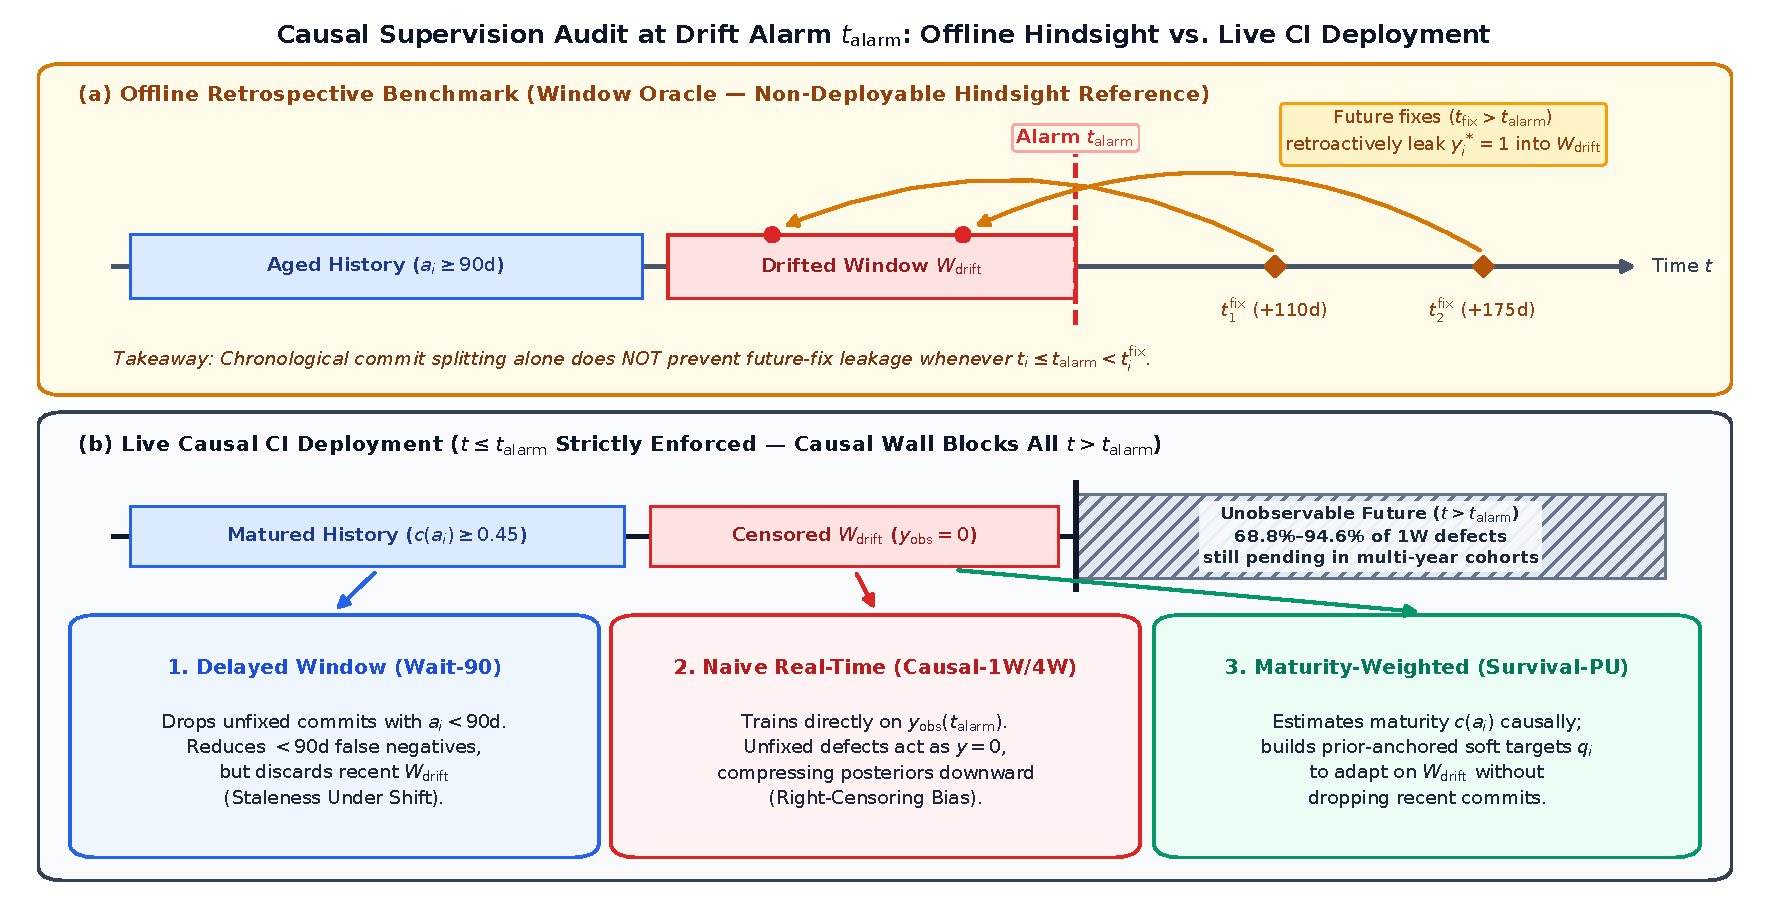
\includegraphics[width=0.98\textwidth]{fig0a_causal_timeline_v3.pdf}
  \caption{Causal supervision audit at drift alarm $t_{\text{alarm}}$: (a) offline retrospective evaluation ($B_{1b}^*$) leaks future SZZ fixes ($t_{\text{fix}} > t_{\text{alarm}}$) into $W_{\text{drift}}$ despite chronological commit ordering; (b) live causal CI deployment ($t \le t_{\text{alarm}}$) confronts the trade-off between delayed $\text{Wait-}90$ (dropping unfixed commits aged $<90\text{d}$) and naive real-time $B_2\text{-1W/4W}$ (treating unfixed defects as $y=0$), addressed via maturity-weighted Bayesian PU targets.}
  \label{fig:causal_timeline}
\end{figure}

\begin{definition}[Causal Label Visibility and Structural Maturity Factorization]
\label{def:observability}
At alarm timestamp $t_{\text{alarm}} = t_e$ on window $W_{\text{drift}} = \{e - W + 1, \dots, e\}$, causal deployment forbids accessing events after $t_{\text{alarm}}$. For any commit $i \le e$ of age $a_i = (t_{\text{alarm}} - t_i)/86400 \ge 0$ (days), its observable label is
\begin{equation}
  y_{i,\text{obs}}(t_{\text{alarm}}) = \mathbb{I}\!\left(y_i^* = 1 \;\wedge\; t_i^{\text{fix}} \le t_{\text{alarm}}\right) = y_i^* \cdot \mathbb{I}\!\left(\Delta_i \le a_i\right).
  \label{eq:y_obs}
\end{equation}
Assume locally on an adaptation window that (A1) latent defect risk is age-stationary given features, $\Pr(y^* = 1 \mid x_i, a_i) = \eta^*(x_i)$, and (A2) reveal delay among true defects is conditionally independent of $x_i$ given age, $\Pr(\Delta \le a_i \mid y^* = 1, x_i, a_i) = c(a_i) \in [0, 1]$. Then $\Pr(y_{\text{obs}} = 1 \mid x_i, a_i) = c(a_i)\,\eta^*(x_i)$.
\end{definition}

\begin{proposition}[Bayes-Optimal Censored Posterior Under Uniform vs.\ Heterogeneous Maturity]
\label{prop:bias}
Under Assumptions~(A1)--(A2) of Definition~\ref{def:observability}, suppose predictor $f_\theta(x)$ minimizes class-weighted binary cross-entropy $\ell(p, y_{\text{obs}}) = -\omega_+ y_{\text{obs}} \log p - (1 - y_{\text{obs}})\log(1 - p)$ ($\omega_+ > 0$) against $y_{\text{obs}}(t_{\text{alarm}})$ over a window with conditional effective maturity $\bar{c}(x) = \mathbb{E}[c(a) \mid x] \in (0, 1]$. For any $x$ with $\eta^*(x) \in (0, 1)$, the population risk minimizer is
\begin{equation}
  \hat{p}_{B_2}(x) = \frac{\omega_+ \, \bar{c}(x) \, \eta^*(x)}{1 - \bar{c}(x)\,\eta^*(x) + \omega_+\,\bar{c}(x)\,\eta^*(x)} = \frac{\omega_+ \, \bar{c}(x) \, \eta^*(x)}{1 + \big(\omega_+ - 1\big)\,\bar{c}(x)\,\eta^*(x)}.
  \label{eq:b2_bayes}
\end{equation}
Equation~\eqref{eq:b2_bayes} implies two structural regimes:
\begin{enumerate}[leftmargin=1.8em,itemsep=0.10em]
  \item \textbf{Constant-Maturity Order Preservation and Exact Threshold Crossing:} If $\bar{c}(x) \equiv \bar{c}_W \in (0, 1)$ is constant across $x$, then $\partial \hat{p}_{B_2} / \partial \eta^* = \omega_+ \bar{c}_W / [1 + (\omega_+ - 1)\bar{c}_W \eta^*]^2 > 0$: population ranking (AP, ROC-AUC) is strictly preserved. Relative to the uncensored ($\bar{c}_W = 1$) weighted minimizer $\hat{p}_{B_1^*}(x) = \omega_+ \eta^*(x)/[1 + (\omega_+ - 1)\eta^*(x)]$, right-censoring strictly reduces $\hat{p}_{B_2}(x) < \hat{p}_{B_1^*}(x)$ (for $\omega_+ = 1$, $\hat{p}_{B_2}(x) = \bar{c}_W \eta^*(x) < \eta^*(x)$), and forces $\hat{p}_{B_2}(x) < \tau_{\text{th}} \in (0, 1)$ if and only if
  \begin{equation}
    \bar{c}_W < \frac{\tau_{\text{th}}}{\eta^*(x)\,\big[\omega_+(1 - \tau_{\text{th}}) + \tau_{\text{th}}\big]}.
    \label{eq:exact_crossing}
  \end{equation}
  \item \textbf{Heterogeneous-Maturity Rank Inversion:} If two feature subpopulations $x_{\text{old}}, x_{\text{new}}$ have effective maturities $\bar{c}(x_{\text{old}}) = c_{\text{hi}} > c_{\text{lo}} = \bar{c}(x_{\text{new}}) > 0$ with $\eta^*(x_{\text{new}}) > \eta^*(x_{\text{old}})$, then $\hat{p}_{B_2}(x_{\text{new}}) < \hat{p}_{B_2}(x_{\text{old}})$ if and only if $\frac{\eta^*(x_{\text{new}})}{1 - c_{\text{lo}}\eta^*(x_{\text{new}})} < \frac{c_{\text{hi}}}{c_{\text{lo}}} \frac{\eta^*(x_{\text{old}})}{1 - c_{\text{hi}}\eta^*(x_{\text{old}})}$.
\end{enumerate}
\end{proposition}

\begin{proof}
Taking conditional expectation under $y_{\text{obs}} \mid x \sim \operatorname{Bernoulli}(\bar{c}(x)\eta^*(x))$ and setting $\partial \mathbb{E}[\ell \mid x]/\partial p = 0$ on $(0, 1)$ gives $\frac{\omega_+ \bar{c}(x)\eta^*(x)}{p} = \frac{1 - \bar{c}(x)\eta^*(x)}{1 - p}$, yielding Eq.~\eqref{eq:b2_bayes}. Differentiating with respect to $\eta^*$ for constant $\bar{c}_W$ proves Claim~1's monotonicity, while solving $\omega_+ \bar{c}_W \eta^*(x) < \tau_{\text{th}}[1 + (\omega_+ - 1)\bar{c}_W \eta^*(x)]$ yields the exact crossing bound~\eqref{eq:exact_crossing}. Comparing strictly monotone odds $\hat{p}_{B_2}/(1 - \hat{p}_{B_2}) = \omega_+ \bar{c}(x)\eta^*(x)/[1 - \bar{c}(x)\eta^*(x)]$ yields Claim~2.
\end{proof}

\textit{Remark (Scope of Proposition~\ref{prop:bias} and Within-Window vs.\ Whole-Stream AP).} Right-censoring does not universally worsen raw Brier error when $\omega_+ > 1$ inflates uncensored posteriors (e.g., at $\eta^* = 0.5, \omega_+ = 4$, $\hat{p}_{B_1^*} = 0.80$ vs.\ $\hat{p}_{B_2} = 0.50$ at $\bar{c}_W = 0.40$). Equally important, Claim~1's monotone ranking preservation holds \textit{within a single window's model}; when predictions across post-alarm windows are concatenated into a single \textit{whole-stream} Precision--Recall curve, inter-window score-scale shifts (such as re-anchoring output scales as estimated priors $\hat{\pi}_{\text{target}}(t)$ or class weights vary) can penalize whole-stream AP even when within-window ranking holds or improves---a cross-window comparability diagnostic we evaluate on $K=25$ in Section~\ref{sec:rq2}. Thus, Proposition~\ref{prop:bias} explains why $B_2\text{-4W}$ can retain competitive whole-stream AP on gradual streams while losing thresholded recall under heavy latency ($\kappa \to 3\times$) and ranking accuracy when shifted features appear at young ages ($c_{\text{lo}} \ll c_{\text{hi}}$).

\subsection{Population Variance of Contiguous vs.\ Independent Draws Under Autocorrelation}
\label{sec:theory_alarm_storm}

Because every triggered alarm exposes the model to right-censored supervision, calibrating the drift monitor to avoid spurious alarms is tightly coupled to update safety. Software commits arrive in serially correlated development bursts (feature sprints, subsystem refactorings, and release freezes), violating the i.i.d.\ sampling assumption of standard uniform bootstrap calibration.

\begin{proposition}[Population Window-Mean Covariance Under Positive Lag Autocovariance]
\label{prop:autocorr}
Let $\{z_t\}_{t \in \mathbb{Z}} \subset \mathbb{R}^d$ be a weakly stationary embedding sequence with mean $\mu_0$, marginal covariance $\Gamma_0 = \operatorname{Cov}(z_t)$, and lag-$k$ autocovariance $\Gamma_k = \operatorname{Cov}(z_t, z_{t+k})$ satisfying $\Delta_\Gamma \triangleq \sum_{k=1}^{W-1}\frac{W-k}{W}(\Gamma_k + \Gamma_k^\top) \succ 0$. Comparing a contiguous window mean $\bar{z}_{\text{contig}} = \frac{1}{W}\sum_{j=1}^W z_{t_0+j}$ against the mean $\bar{z}_{\text{ind}} = \frac{1}{W}\sum_{j=1}^W \tilde{z}_j$ of $W$ independent draws $\tilde{z}_j$ from the same marginal law, $\operatorname{Cov}(\bar{z}_{\text{contig}}) = \operatorname{Cov}(\bar{z}_{\text{ind}}) + \frac{1}{W}\Delta_\Gamma \succ \operatorname{Cov}(\bar{z}_{\text{ind}})$ and $\mathbb{E}\|\bar{z}_{\text{contig}} - \mu_0\|_2^2 > \mathbb{E}\|\bar{z}_{\text{ind}} - \mu_0\|_2^2$.
\end{proposition}

\begin{proof}
Expanding $\operatorname{Cov}(\frac{1}{W}\sum_{j=1}^W z_{t_0+j}) = \frac{1}{W}\Gamma_0 + \frac{1}{W^2}\sum_{k=1}^{W-1}(W-k)(\Gamma_k + \Gamma_k^\top)$ whereas $\operatorname{Cov}(\bar{z}_{\text{ind}}) = \frac{1}{W}\Gamma_0$ gives difference $\frac{1}{W}\Delta_\Gamma \succ 0$ and trace gap $\frac{1}{W}\operatorname{tr}(\Delta_\Gamma) > 0$.
\end{proof}

In finite calibration pools of size $N_{\text{cal}}$, uniform bootstrap resampling replaces $\Gamma_0$ with the empirical pool covariance $\hat{\Sigma}_{\text{pool}}$ while breaking lag-$k$ sprint serial correlation ($k \ge 1$) \citep{kunsch1989jackknife,politis1992circular}. Although Proposition~\ref{prop:autocorr} characterizes the mean-shift component rather than the full nonlinear Gaussian Fr\'echet statistic, it motivates calibrating DriftLens via circular contiguous blocks ($b = \max(\min(\lfloor W/6 \rfloor, 80), 25)$). To separate bootstrap sampling from post-alarm updating without confounding percentile or cooldown settings, our RQ4b experiment evaluates a clean $2 \times 2$ factorial at fixed $(d_{\text{pca}}=24, p_{95}, \text{cooldown}=1)$ crossing $\{\text{IID}, \text{Circular Block}\}$ with $\{\text{Static}, \text{Rolling Ref+Th}\}$, where Rolling Ref+Th refreshes reference statistics on the trailing $3W$ commits upon alarms and blends the recalibrated $p_{95}$ threshold ($0.70\,\tau_{\text{new}} + 0.30\,\tau_{\text{old}}$), alongside Pote et al.'s static $(p_{98}, \text{cooldown}=0)$ reference.

% ============================================================================
% 4. Methodology: Three-Stage Survival-PU Adaptation Protocol
% ============================================================================
\section{Methodology: Three-Stage Survival-PU Adaptation Protocol}
\label{sec:method}

Proposition~\ref{prop:bias} indicates that safe real-time adaptation at alarm timestamp $t_{\text{alarm}}$ requires resolving three coupled obstacles using only past repository state ($t_i \le t_{\text{alarm}}$): (1) estimating commit-age reveal maturity $c(a_i)$ without conditioning naively on fast-revealing fixes; (2) estimating target defect prevalence $\hat{\pi}_{\text{target}}$ and a reliable teacher ranking without exploding variance on young commits; and (3) training on the full adaptation pool $\mathcal{B} = \mathcal{A}_{\text{anc}} \cup W_{\text{drift}}$ with soft targets that preserve fresh drift signals while preventing posterior collapse.

Figure~\ref{fig:architecture} summarizes the resulting gate-free three-stage \textbf{Survival-PU} pipeline, and Table~\ref{tab:hyperparams} consolidates every locked protocol parameter frozen prior to unlocking the confirmatory repositories (exact code symbol mappings appear in Appendix~\ref{app:repro}). Preliminary heuristic three-state safety gates are excluded from the core method and isolated strictly as an ablation control (\texttt{Survival-PU (+Legacy Gate)}).

\begin{figure}[!htb]
  \centering
  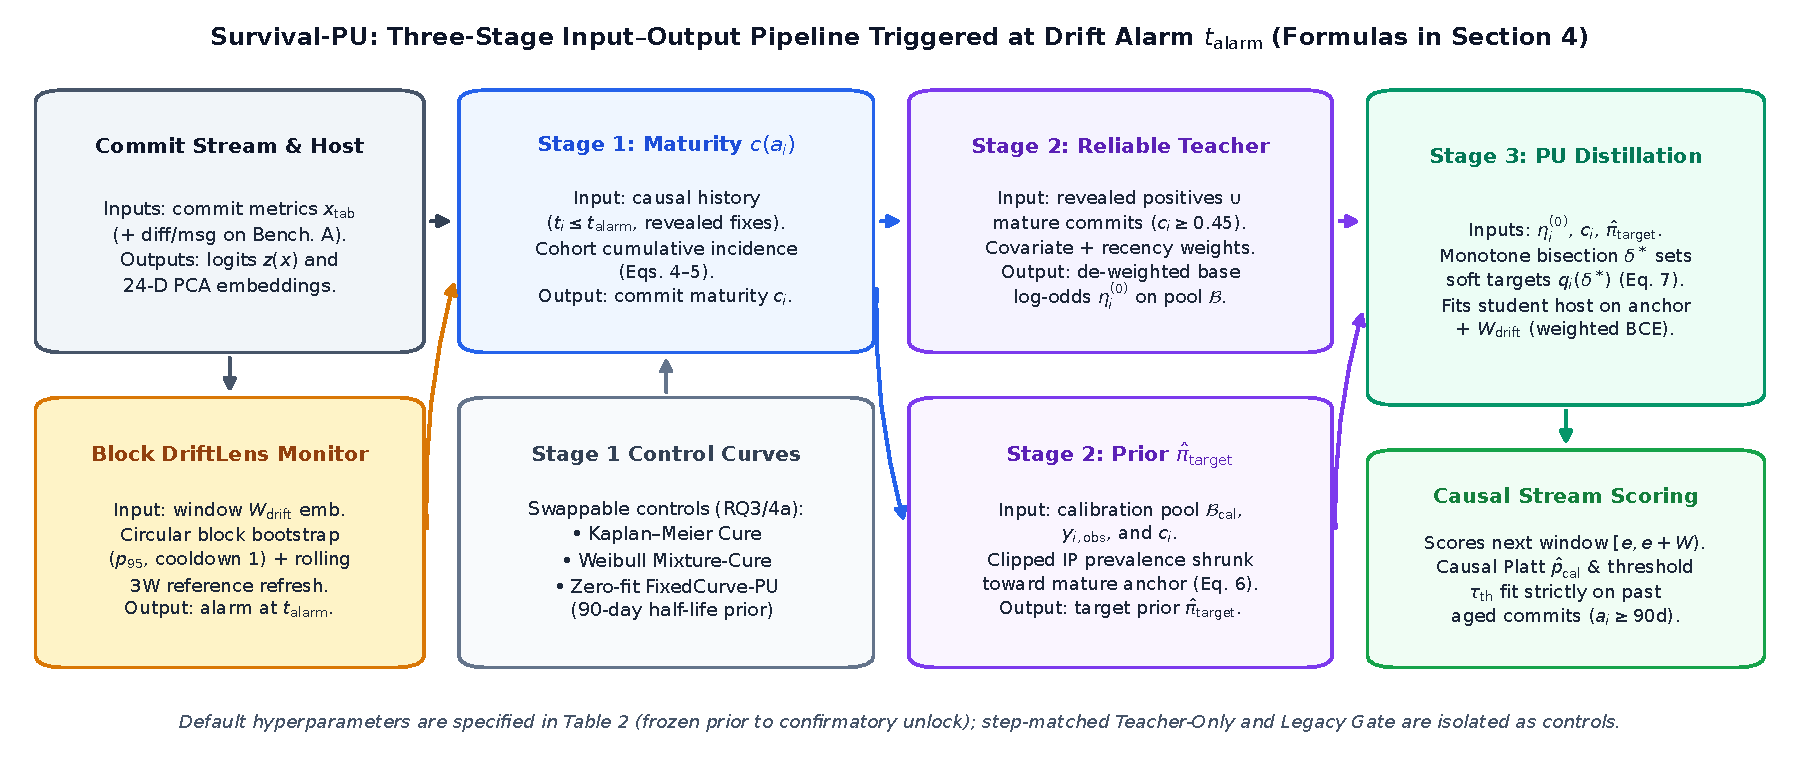
\includegraphics[width=0.98\textwidth]{fig0b_survival_pu_architecture_v3.pdf}
  \caption{Three-stage input--output pipeline of Survival-PU at each DriftLens alarm $t_{\text{alarm}}$: (Stage~1) risk-eligible cohort cumulative incidence $c_i$ on trailing history $\mathcal{H}_{\text{rec}}$; (Stage~2) reliable teacher $T_\phi$ ($85/15$ blend initialization on neural hosts; fresh $75$-tree fit on LightGBM) and clipped inverse-maturity shrunk prevalence $\hat{\pi}_{\text{target}}$ ($\tilde{c}_i = \max(c_i, 0.10)$) on $\mathcal{B}_{\text{cal}} \subset \mathcal{B}$; and (Stage~3) monotone bisection on $\mathcal{B}_{\text{cal}}$ producing maturity- and prior-adjusted soft targets $q_i(\delta^*)$ across $\mathcal{B} = \mathcal{A}_{\text{anc}} \cup W_{\text{drift}}$.}
  \label{fig:architecture}
\end{figure}

\begin{table}[!htb]
\centering
\caption{Locked protocol parameters of Survival-PU and DriftLens frozen prior to unlocking the confirmatory repositories (exact module and configuration object mappings appear in Appendix~\ref{app:repro}).}
\label{tab:hyperparams}
\fontsize{6.0}{7.2}\selectfont
\renewcommand{\arraystretch}{1.02}
\setlength{\tabcolsep}{1.8pt}
\begin{tabularx}{\textwidth}{lccL{2.95cm}Y}
\toprule
\textbf{Module} & \textbf{Symbol} & \textbf{Default} & \textbf{Config Field} & \textbf{Executed Statistical / Operational Role} \\
\midrule
Stage 1 & $N_{\text{hist}}, q_{\max}$ & $6{,}000,\; 0.85$ & \texttt{max\_\allowbreak history\_\allowbreak cohort}, \texttt{support\_\allowbreak age\_\allowbreak quantile} & Trailing cohort slice $[-N_{\text{hist}}:]$ and $85\%$ age support $a_{\max}$ \\
Stage 1 & $n_{\min}^{\text{risk}}, n_{\min}^{\text{fix}}$ & $120,\; 15$ & \texttt{min\_\allowbreak risk\_\allowbreak set}, \texttt{min\_\allowbreak observed\_\allowbreak fixes} & Risk-set floor ($\ge 25$) and fix floor before $0.88(1 - 2^{-a/90})$ fallback \\
Stage 1 & $[c_{\min}, c_{\max}]$ & $[0.05, 0.96]$ & \texttt{c\_min}, \texttt{c\_max} & Pre- and post-interpolation maturity bounds across Stage~1 estimators \\
Stage 1 & $[\gamma_{\min}, \gamma_{\max}]$ & $[0.60, 0.94]$ & \texttt{tail\_\allowbreak cap\_\allowbreak min}, \texttt{tail\_\allowbreak cap\_\allowbreak max} & Finite-horizon tail-completeness cap bounds (swept in RQ4d) \\
Stage 2 & $\tau_{\text{rel}}, N_{\text{rel}}$ & $0.45,\; 2{,}200$ & \texttt{reliable\_\allowbreak maturity\_\allowbreak thresh}, \texttt{max\_\allowbreak reliable\_\allowbreak commits} & Reliable cohort $\mathcal{R} = \{y_{\text{obs}}=1 \vee c_i \ge 0.45\}$ trailing cap \\
Stage 2 & $[w_{\min}, w_{\max}]$ & $[0.50, 2.50]$ & \texttt{imp\_\allowbreak weight\_\allowbreak min}, \texttt{imp\_\allowbreak weight\_\allowbreak max} & $L_2$-logistic domain density-ratio clipping bounds \\
Stage 2 & $c_{\text{ht}}, m_0, [\pi_{\min}, \pi_{\max}]$ & $0.10, 50, [0.02, 0.70]$ & \texttt{ht\_\allowbreak floor\_\allowbreak c}, \texttt{ht\_\allowbreak shrinkage\_\allowbreak m0}, \texttt{pi\_min}, \texttt{pi\_max} & Inverse-maturity floor $\tilde{c}_i = \max(c_i, 0.10)$ and $n_{\text{eff,heur}}$ shrinkage on $\mathcal{B}_{\text{cal}}$ \\
Stage 2 & $\tau_{\text{sharp}}, \beta_{\text{LLM}}$ & $1.15,\; 0.25$ & \texttt{teacher\_\allowbreak sharpness}, \texttt{llm\_\allowbreak blend\_\allowbreak weight} & Teacher prior-adjusted logit scaling and optional RQ4e LLM blend \\
Stage 3 & $N_{\text{anc}}, \gamma_{\text{drift}}, u_0$ & $2{,}000,\; 1.40,\; 0.45$ & \texttt{max\_\allowbreak anchor\_\allowbreak commits}, \texttt{drift\_\allowbreak emphasis\_\allowbreak gamma}, \texttt{maturity\_\allowbreak weight\_\allowbreak floor} & Non-drift anchor cap, $W_{\text{drift}}$ emphasis, and maturity weight floor $u_i$ \\
Stage 3 & $[p_{\min}, p_{\max}], K_{\text{bis}}$ & $[0.003, 0.997],\; 28$ & \texttt{posterior\_\allowbreak p\_\allowbreak min}, \texttt{posterior\_\allowbreak p\_\allowbreak max}, \texttt{bisection\_\allowbreak iters} & Shared posterior clamp and monotone bisection iterations on $[-8, 8]$ \\
Budgets & $R_{\text{init}}, R_{\text{alm}}$ & $90,\; 75$ & \texttt{lgb\_\allowbreak init\_\allowbreak rounds}, \texttt{lgb\_\allowbreak alarm\_\allowbreak rounds} & LightGBM init ($90$) and fresh per-stage alarm ($75$; Teach-Matched $=150$) rounds \\
Budgets & $E_{\text{teach}}, E_{\text{stud}}, \eta$ & $4,\; 4,\; 4.5\text{e-}4$ & \texttt{neural\_\allowbreak teacher\_\allowbreak epochs}, \texttt{neural\_\allowbreak student\_\allowbreak epochs}, \texttt{neural\_\allowbreak adapt\_\allowbreak lr} & Neural SPU ($4+4$) epochs (init $=12$, $B_2$/Wait $=5$, $\text{nnPU}=6$) \\
Monitor & $W, d_{\text{pca}}, p_{\text{blk}}, \text{cd}$ & $400,\; 24,\; 95.0,\; 1$ & \texttt{window\_\allowbreak size\_\allowbreak default}, \texttt{drift\_\allowbreak pca\_\allowbreak dim}, \texttt{drift\_\allowbreak block\_\allowbreak pct}, \texttt{drift\_\allowbreak cooldown\_\allowbreak windows} & Default window size, PCA dim, percentile, and cooldown ($2\times 2$ factorial) \\
\bottomrule
\end{tabularx}
\end{table}

\subsection{Stage 1: Risk-Eligible Cohort Cumulative Incidence and Survival Controls}
\label{sec:stage1}

A naive empirical CDF over observed bug fixes ($y_{i,\text{obs}} = 1$) severely underestimates fix latency because slow-revealing bugs are systematically absent from recent commits. To avoid this right-truncation bias, Stage~1 slices the trailing $N_{\text{hist}}$ causal commits $\mathcal{H}_{\text{rec}} \subset \{i : t_i \le t_{\text{alarm}}\}$ \textit{before} computing age quantiles, recording commit age $a_i = \max((t_{\text{alarm}} - t_i)/86400, 0)$ and observed fix delay $d_i = \max((t_i^{\text{fix}} - t_i)/86400, 0)$ solely when $y_{i,\text{obs}}(t_{\text{alarm}}) = 1$ (with $d_i = +\infty$ otherwise, quarantining any retroactive $t_i^{\text{fix}} < t_i$ to $+\infty$). On candidate age knots $g_0 = 0 < g_1 < \dots < g_M = a_{\max}$ up to the support quantile $a_{\max} = Q_{q_{\max}}(\{a_i\}_{i \in \mathcal{H}_{\text{rec}}})$, with effective risk-set floor $n_{\text{eff}}^{\text{risk}} = \max(\min(n_{\min}^{\text{risk}}, \lfloor (1 - q_{\max})|\mathcal{H}_{\text{rec}}| \rfloor), 25)$, the \textbf{Risk-Eligible Cohort Cumulative Incidence Estimator} restricts each knot's denominator to commits old enough to be observed at lag $g_m$, $\mathcal{E}(g_m) = \{i \in \mathcal{H}_{\text{rec}} : a_i \ge g_m\}$ (carrying forward $\hat{G}(g_{m-1})$ when $|\mathcal{E}(g_m)| < n_{\text{eff}}^{\text{risk}}$ for $m > 0$), and enforces monotonicity via its running maximum:
\begin{equation}
  \hat{G}(g_m) = \frac{1}{|\mathcal{E}(g_m)|}\sum_{i \in \mathcal{E}(g_m)} \mathbb{I}\!\left(y_{i,\text{obs}} = 1 \;\wedge\; d_i \le g_m\right), \qquad \tilde{G}(g_m) = \max_{0 \le k \le m}\hat{G}(g_k).
  \label{eq:cohort_inc}
\end{equation}

Because $\tilde{G}(a_{\max})$ still reflects finite-horizon observation up to $a_{\max}$, Stage~1 rescales the normalized curve by a bounded tail-completeness factor $\gamma_{\text{tail}} \in [\gamma_{\min}, \gamma_{\max}]$. Letting $\tilde{G}_{\text{half}} = \operatorname{interp}(0.5\,a_{\max}; \{g_m\}, \{\tilde{G}(g_m)\})$, the growth ratio is $r_g = \tilde{G}(a_{\max}) / \tilde{G}_{\text{half}}$ when $\tilde{G}_{\text{half}} > 10^{-5}$ and $r_g = 1.5$ otherwise; combining this with age factor $\phi_a = \operatorname{clip}(a_{\max}/(a_{\max}+45),\, 0.65,\, 1.0)$ yields $\gamma_{\text{tail}} = \operatorname{clip}([\gamma_{\max} - 0.28\operatorname{clip}(r_g - 1, 0, 1)]\,\phi_a,\, \gamma_{\min},\, \gamma_{\max})$. Knot maturities are clipped \textit{prior} to piecewise-linear interpolation across knots:
\begin{equation}
  \begin{aligned}
    c_{\text{knot}}(g_m) &= \operatorname{clip}\!\Big(\gamma_{\text{tail}}\,\frac{\tilde{G}(g_m)}{\tilde{G}(a_{\max})},\; c_{\min},\; c_{\max}\Big), \\
    c_i &= \operatorname{clip}\!\big(\operatorname{interp}(a_i;\, \{g_m\}, \{c_{\text{knot}}(g_m)\}),\; c_{\min},\; c_{\max}\big),
  \end{aligned}
  \label{eq:ci_interp}
\end{equation}
with left boundary $c_{\min}$ and right boundary $c_{\text{knot}}(g_M)$. Whenever historical support is insufficient (observed fixes $< n_{\min}^{\text{fix}}$, $|\mathcal{H}_{\text{rec}}| < 200$, $a_{\max} < 30\text{d}$, or $\tilde{G}(a_{\max}) < 10^{-4}$), the estimator activates a deterministic fallback that evaluates $0.88(1 - 2^{-g/90})$ on $145$ uniform knots spanning $[0, 720]$ days ($5\text{-day}$ spacing), clips those knot values to $[c_{\min}, c_{\max}]$, and piecewise-linearly interpolates at $a_i$ (holding the terminal $720\text{-day}$ knot value for $a_i > 720\text{d}$).

To test whether learned survival curves improve upon classical survival estimators or a zero-fit parametric prior, RQ2 and RQ3 compare three alternatives under the identical Stage~1 interface: (i) right-censored \textbf{Kaplan--Meier Cure}, quantizing event and censoring times onto a shared $10^{-4}$-day ($\approx 8.6\text{ s}$) grid so the risk-set invariant $0 \le e_u \le n_u$ holds identically; (ii) L-BFGS-B \textbf{Weibull Mixture-Cure MLE} \citep{boag1949cure,farewell1982cure} fitted on unstratified $\mathcal{H}_{\text{rec}}$ (a global Weibull delay family containing the exponential special case at shape $k=1$, inspired by delayed-feedback/cure likelihoods rather than jointly fitting feature-dependent $p(x)$ and $\lambda(x)$ as in \citet{chapelle2014modeling}); and (iii) zero-fit \textbf{FixedCurve-PU}, setting $c_{\text{fix}}(a_i) = \operatorname{clip}(1 - 2^{-a_i/90},\, c_{\min},\, c_{\max})$.

\textit{Identifiability Assumptions of Stage~1.} Because the denominator of Eq.~\eqref{eq:cohort_inc} includes all age-eligible commits, $\hat{G}(a)$ estimates the joint probability $\pi F_\Delta(a)$ rather than conditional maturity $c(a) = F_\Delta(a)$ directly. Canceling $\pi$ in Eq.~\eqref{eq:ci_interp} therefore relies on two structural assumptions: (I1) trailing-cohort defect prevalence $\pi$ and delay distribution $F_\Delta$ are locally stationary across commit ages inside $\mathcal{H}_{\text{rec}}$, and (I2) $\gamma_{\text{tail}}$ approximates terminal completeness at $a_{\max}$. Under abrupt prevalence shifts across cohorts, $\hat{G}(a)$ can confound lower defect prevalence with slower reveal---an effect we audit directly against post hoc empirical $c^*(a)$ across 62 fired alarms in Section~\ref{sec:rq3} and Table~\ref{tab:mechanism_audit}.

\subsection{Stage 2: Clipped Inverse-Maturity Prevalence on \texorpdfstring{$\mathcal{B}_{\text{cal}}$}{B\_cal} and Reliable Teacher}
\label{sec:stage2}

At each alarm, we construct the adaptation pool $\mathcal{B} = \mathcal{A}_{\text{anc}} \cup W_{\text{drift}}$ by pairing the trailing $N_{\text{anc}}$ non-drift commits $\mathcal{A}_{\text{anc}}$ with the newly flagged window $W_{\text{drift}}$. To account for covariate shift between historical anchors and the shifted window, an $L_2$-regularized domain logistic classifier discriminates $\mathcal{A}_{\text{anc}}$ from $W_{\text{drift}}$ to yield bounded importance weights $w_{\text{imp}}(x_i) \in [w_{\min}, w_{\max}]$ \citep{sugiyama2008direct}. Multiplying $w_{\text{imp}}(x_i)$ on $\mathcal{A}_{\text{anc}}$ by linear recency in $[0.70, 1.15]$ while assigning uniform emphasis $w_i = \gamma_{\text{drift}}$ on $W_{\text{drift}}$ yields base weights $w_i$ and observation-independent sample weights $u_i = w_i[u_0 + (1 - u_0)c_i]$.

Directly dividing observed labels $y_{i,\text{obs}}$ by $c_i$ to estimate target prevalence incurs extreme variance on very young commits ($c_i \approx 0.05$). Stage~2 therefore operates on the trailing calibration subset $\mathcal{B}_{\text{cal}} \subset \mathcal{B}$ of size $N_{\text{cal}} = \min(|\mathcal{B}|, \max(3|W_{\text{drift}}|, 900))$ using an inverse-maturity floor $\tilde{c}_i = \max(c_i, c_{\text{ht}})$ ($c_{\text{ht}} = 0.10$), combining a clipped inverse-maturity plug-in estimator with heuristic variance-inflation shrinkage toward a mature anchor prior $\pi_{\text{anc}}$:
\begin{equation}
  \begin{aligned}
    \hat{\pi}_{\text{IP}} &= \frac{\sum_{i \in \mathcal{B}_{\text{cal}}} u_i\,(y_{i,\text{obs}} / \tilde{c}_i)}{\sum_{i \in \mathcal{B}_{\text{cal}}} u_i}, \qquad n_{\text{eff,heur}} = \frac{\big(\sum_{i \in \mathcal{B}_{\text{cal}}} u_i\big)^2}{\sum_{i \in \mathcal{B}_{\text{cal}}} (u_i / \tilde{c}_i)^2}, \\
    \hat{\pi}_{\text{target}} &= \operatorname{clip}\!\left(\max\!\left(\frac{n_{\text{eff,heur}}\,\hat{\pi}_{\text{IP}} + m_0\,\pi_{\text{anc}}}{n_{\text{eff,heur}} + m_0},\; \bar{y}_{\text{obs},\mathcal{B}_{\text{cal}}} + 10^{-4}\right),\; \pi_{\min},\; \pi_{\max}\right).
  \end{aligned}
  \label{eq:ht_prev}
\end{equation}
Here $\pi_{\text{anc}}$ is the inverse-maturity mean over mature history $\{j : c_j \ge 0.55\}$ when at least $80$ commits qualify (otherwise the initial pre-stream anchor prevalence), $\bar{y}_{\text{obs},\mathcal{B}_{\text{cal}}} = \sum_{i \in \mathcal{B}_{\text{cal}}} u_i y_{i,\text{obs}} / \sum_{i \in \mathcal{B}_{\text{cal}}} u_i$, and commits with $c_i < c_{\text{ht}}$ incur conservative downward attenuation $c_i / c_{\text{ht}}$. Note a concrete mathematical boundary condition in Eq.~\eqref{eq:ht_prev}: because the outer clamp $[\pi_{\min}, \pi_{\max}] = [0.02, 0.70]$ wraps $\max(\cdot, \bar{y}_{\text{obs},\mathcal{B}_{\text{cal}}} + 10^{-4})$, whenever $\bar{y}_{\text{obs},\mathcal{B}_{\text{cal}}} > 0.70$, the target is capped at $0.70 < \bar{y}_{\text{obs},\mathcal{B}_{\text{cal}}}$ and becomes algebraically unreachable in Stage~3 (because Eq.~\eqref{eq:bayes_pu} sets $q_i = 1$ on revealed positives and $q_i \ge 0$ elsewhere). We audit the exact empirical frequency of this unreachable regime across all experiments in Section~\ref{sec:stage3}.

In parallel, Stage~2 trains a teacher classifier $T_\phi$ on the trailing $N_{\text{rel}}$ commits of the selective reliable cohort $\mathcal{R} = \{i : y_{i,\text{obs}} = 1 \vee c_i \ge \tau_{\text{rel}}\}$ (when $|\mathcal{R}| \ge 100$) so that unfixed commits with low maturity do not dominate teacher feature weights. Teacher samples carry weight $w_{\text{rel},i} = w_{\text{imp}}(x_i)\cdot r_{\text{conf},i}\cdot \text{recency}_i$, where $r_{\text{conf},i} = 0.55 + 0.45 c_i$ if $y_{i,\text{obs}} = 1 \wedge c_i < \tau_{\text{rel}}$ (else $1$) and $\text{recency}_i \in [0.75, 1.15]$, with positive class weight $\omega_{+,\text{teach}} = \frac{1}{2}\omega_+ + \frac{1}{2}\operatorname{clip}((1-\hat{\pi}_{\text{target}})/\max(\hat{\pi}_{\text{target}}, 0.03), 1.5, \max(4.5, \omega_+))$. Host initialization follows each model family's native paradigm: on \textbf{neural hosts}, $T_\phi$ initializes from an $85\%/15\%$ parameter blend of the current checkpoint and the initial pre-stream anchor and trains for $E_{\text{teach}}$ epochs; on \textbf{LightGBM}, the teacher fits a fresh $R_{\text{alm}}$-tree booster without inheriting prior trees or margins. Either host emits class-weight-adjusted base log-odds $\eta_i^{(0)} = \tau_{\text{sharp}}(z_{\text{teach}}(x_i) - \log \omega_{+,\text{teach}})$ across $\mathcal{B}$. Crucially, subtracting $\log \omega_{+,\text{teach}}$ removes explicit class reweighting but does \textit{not} eliminate selective-cohort inclusion bias on young commits or residual censoring among commits with $c_i \ge 0.45$; accordingly, Stage~3 treats $q_i(\delta^*)$ strictly as \textit{maturity- and prior-adjusted soft targets} rather than exact true posteriors (audited by commit age in Section~\ref{sec:rq3}).

\subsection{Stage 3: Maturity- and Prior-Adjusted Soft Targets, Linear-Residual Skip, and Callable LightGBM}
\label{sec:stage3}

To transfer knowledge from matured history onto the entire adaptation pool $\mathcal{B}$---including fresh commits in $W_{\text{drift}}$---Stage~3 constructs maturity- and prior-adjusted soft targets via a single shared mapping $(\eta_i^{(0)}, \delta, y_{i,\text{obs}}, c_i)$ setting $q_i(\delta) = 1$ whenever $y_{i,\text{obs}} = 1$ and, for unrevealed commits ($y_{i,\text{obs}} = 0$),
\begin{equation}
  q_i(\delta) = \frac{\tilde{p}_i(\delta)\,(1 - c_i)}{1 - \tilde{p}_i(\delta)\,c_i}, \qquad \tilde{p}_i(\delta) = \operatorname{clip}\!\big(\sigma(\eta_i^{(0)} + \delta),\; p_{\min},\; p_{\max}\big).
  \label{eq:bayes_pu}
\end{equation}
Conditional on equal maturity $c_i$ among unrevealed commits ($y_{i,\text{obs}} = 0$), $q_i(\delta)$ is nondecreasing in $\eta_i^{(0)}$ and strictly increasing on the unclipped interior $\sigma(\eta_i^{(0)} + \delta) \in (p_{\min}, p_{\max})$; across heterogeneous ages, it downweights aged unfixed commits ($q_i \to 0$ as $c_i \to 1$) relative to fresh unfixed commits ($q_i \to \tilde{p}_i$ as $c_i \to 0$). Letting $f(\delta) = \sum_{i \in \mathcal{B}_{\text{cal}}} u_i q_i(\delta) / \sum_{i \in \mathcal{B}_{\text{cal}}} u_i$, monotone bisection ($K_{\text{bis}}$ iterations on $[-8, 8]$) targets $f(\delta^*) = \hat{\pi}_{\text{target}}$ on $\mathcal{B}_{\text{cal}}$ whenever $\hat{\pi}_{\text{target}} \in [f(-8), f(+8)]$. When $\hat{\pi}_{\text{target}}$ falls outside this reachable interval---determined by the alarm-time weighted observed positive rate $\bar{y}_{\text{obs},\mathcal{B}_{\text{cal}}}$ and teacher logit saturation inside $\mathcal{B}_{\text{cal}}$ (e.g., if $\bar{y}_{\text{obs},\mathcal{B}_{\text{cal}}} > \pi_{\max} = 0.70$)---the target is not matched exactly; instead, the solver returns the nearest boundary $\delta^* \in \{-8, +8\}$, achieving endpoint mean $f(\delta^*)$ with residual $|f(\delta^*) - \hat{\pi}_{\text{target}}|$, and logs an unreachable solve. Auditing all runs with total-alarm denominators confirms $0$ unreachable solves on Benchmark~A and RQ4a--e; across all 27 Benchmark~B natural streams, $1.0 / 161.7$ alarms ($0.62\%$) were unreachable, concentrated in \texttt{apache\_flink} ($0.1 / 6.5 = 1.5\%$) and \texttt{apache\_groovy} ($0.9 / 5.4 = 16.7\%$, coinciding with $0.9$ survival fallbacks); on Confirmatory \texttt{HDFS*}, high alarm-time $\bar{y}_{\text{obs},\mathcal{B}_{\text{cal}}}$ triggered unreachable clamping on $0.4 / 1.4 = 28.6\%$ of MLP alarms and $0.6 / 2.0 = 30.0\%$ of LightGBM alarms (illustrating that production implementations should raise $\pi_{\max}$ above $\bar{y}_{\text{obs},\mathcal{B}_{\text{cal}}}$ or project $\hat{\pi}_{\text{target}}$ onto $[f(-8), f(+8)]$). Float32 soft targets $q_i(\delta^*)$ then train the student across $\mathcal{B}$ under $\mathcal{L}_{\text{SPU}}(z) = \sum_{i \in \mathcal{B}} u_i [\omega_{+,\text{teach}} q_i(\delta^*) \log(1 + e^{-z_i}) + (1 - q_i(\delta^*))\log(1 + e^{z_i})]$, initializing neural students from $T_\phi$ ($E_{\text{stud}}$ epochs) and fitting fresh $R_{\text{alm}}$-tree LightGBM boosters (matched in total trees $R_{\text{alm}} + R_{\text{alm}}$ against single-stage $2R_{\text{alm}}$-tree \texttt{Teacher-Only (Matched)}).

Two host-level mechanisms ensure consistent execution across multimodal neural encoders and gradient-boosted trees:
\begin{enumerate}[leftmargin=1.8em,itemsep=0.10em]
  \item \textbf{Causal Tabular Linear-Residual Skip Connection (Multimodal Neural Backbones):} Because high-dimensional diff and message encoders can dilute commit-size predictors (\texttt{la}, \texttt{nf}, \texttt{ent}) \citep{zeng2021deep}, neural hosts support $z(x) = w_{\text{LR}}^\top x_{\text{tab}} + b_{\text{LR}} + f_\theta(x)$, where $(w_{\text{LR}}, b_{\text{LR}})$ are fitted via $L_2$-regularized logistic regression on $[0, n_{\text{init}}+n_{\text{val}})$ using $y_{\text{obs}}(t_{\text{start}})$ (while scalers and token vocabularies fit strictly on $[0, n_{\text{init}})$) and $f_\theta$'s output head is zero-initialized. Pre-stream validation selected a frozen linear skip over a trainable skip ($0.0586$ vs.\ $0.0575$ validation AP).
  \item \textbf{Analytical Callable Objective for Gradient-Boosted Trees \citep{friedman2001greedy,ke2017lightgbm}:} Rather than duplicating rows $2|\mathcal{B}|$ times, our LightGBM host supplies exact continuous-target first and second derivatives ($g_i, h_i$) with initial margin $z_{\text{init}} = \log(\bar{p}_0 / (1 - \bar{p}_0))$ propagated identically to inference (derivation and verification details in Appendix~\ref{app:repro}, Proposition~\ref{prop:lgbm}).
\end{enumerate}

% ============================================================================
% 5. Experimental Design & Statistical Protocol
% ============================================================================
\section{Experimental Design and Evaluation Protocol}
\label{sec:setup}

To separate development analysis from out-of-sample replication, we structured benchmark evaluation into three tiers, froze all modeling and statistical code prior to unlocking an initially untouched confirmatory cohort, and verified pipeline prefix invariance across every method execution branch. Throughout this study, we distinguish: (i) \textit{protocol-specified development-cohort analyses} on Benchmark~A and Benchmark~B ($K=25$, whose comparison families and decision rules were codified in our codebase prior to confirmatory unlock rather than externally timestamp-preregistered before all development exploration); (ii) \textit{pre-unlock frozen confirmatory evaluation} on five initially absent ApacheJIT repositories; and (iii) one \textit{post-unlock split-sizing amendment} for small streams ($N < 4{,}000$), disclosed explicitly below.

\subsection{Provenance-Audited Stream Tiers, Data-Construction Funnels, and Archive Follow-Up}
\label{sec:benchmarks}

Our evaluation spans \textbf{37 development streams} (6 Benchmark~A multimodal streams, 27 natural Benchmark~B streams, and 4 Benchmark~B controlled concatenated-shift streams; 89 archived stream bundles total) plus \textbf{5 confirmatory ApacheJIT repositories}, totaling 347,122 natural repository commit records alongside a paired Code-LLM prompting case study:

\begin{enumerate}[leftmargin=1.8em,itemsep=0.14em]
  \item \textbf{Benchmark A — Multimodal Qt (25,704 Commits) and OpenStack (13,304 Commits; 6 Streams):} Cross-linking DeepJIT corpora \citep{hoang2019deepjit}, the tables of \citet{mcintosh2018are}, and 16 official Git repositories, we verified Tier~1+2 cryptographic SZZ bug-fixing timestamps for \textbf{96.49\%} ($1{,}761/1{,}825$; median lag $163.1\text{d}$) of Qt defects and \textbf{99.32\%} ($1{,}616/1{,}627$; median $178.7\text{d}$) of OpenStack defects, quarantining heuristic Tier-3 matches and unlinked defects to $t_{\text{fix}} = +\infty$. Primary streams retain \textbf{only the 13 commit-authoring metrics} (\texttt{la}, \texttt{ld}, \texttt{nf}, \texttt{nd}, \texttt{ns}, \texttt{ent}, \texttt{ndev}, \texttt{age}, \texttt{nuc}, \texttt{aexp}, \texttt{arexp}, \texttt{asexp}, \texttt{asawr}), removing 15 post-authoring Gerrit review fields (isolated in pre-merge sensitivity streams). \textit{Archival merged-commit caveat:} raw Qt/OpenStack tables provide only \texttt{author\_date} without Gerrit patch-set-1 upload or merge timestamps; thus Benchmark~A models \textit{archival merged-commit replay}, not initial unreviewed patch-set-1 pushes. Empty diffs (Qt: 262 commits, $1.02\%$; OpenStack: 10 commits, $0.08\%$) are encoded strictly as empty strings without message substitution. Across two natural ecosystems and four controlled subsystem shifts, we evaluate \textbf{Attention-CNN} \citep{pote2026adaptive}, \textbf{CodeBERT} \citep{feng2020codebert}, \textbf{DeepJIT-CNN} \citep{hoang2019deepjit}, and \textbf{LightGBM} \citep{ke2017lightgbm} (5 seeds) plus all 11 Track~2 baselines.
  \item \textbf{Benchmark B — 27 Natural Streams ($K=25$ Independent Donor Clusters, 300,637 Commits) plus 4 Controlled Concatenated Shifts:} Combines 14 CommitGuru streams from \citet{cabral2019class}, eight ApacheJIT development streams \citep{keshavarz2022apachejit}, and five PR-SZZ streams from \citet{bludau2026quantifying} (ordered by Git committer date after removing 13 post-closure/target columns and mapping post-2021H1 sentinels to $+\infty$). Merging Apache Camel (shared by CommitGuru and ApacheJIT) and OpenStack Nova/Neutron maps the 27 natural streams onto \textbf{$K=25$ independent donor clusters} (and Benchmark-A-disjoint \textbf{$K=24$}). Four \textit{controlled concatenated distribution-shift streams} (Nova$\to$Zulip, Ignite$\to$Cassandra, Airflow$\to$Pulsar, and OpenStack Nova$\to$Neutron) are kept strictly outside $K=25$ natural inference (10 MLP seeds, all Track~2 learners, 5 LightGBM seeds). \textit{Exact splice timeline construction:} concatenating a pre-shift prefix and post-shift suffix shifts all post-onset commit timestamps and finite fix timestamps by $\Delta t = t_{\text{pre,last}} - t_{\text{post,first}} + 3{,}600\text{ s}$ (a fixed 1-hour boundary gap; $+\infty$ remains $+\infty$), while $23.7\%\text{--}60.0\%$ of revealed pre-onset fixes continue arriving after the onset boundary (Appendix Table~\ref{tab:shift_4streams}); these streams are therefore controlled cross-project distribution-shift benchmarks rather than natural single-repo concept drift.
  \item \textbf{Phase C — Confirmatory ApacheJIT Cohort ($K=4$ Umbrella Ecosystems / 5 Repositories, 7,477 Commits) and Upstream Monorepo Disclosure:} Prior to downloading official \texttt{apachejit\_total.csv} ($106{,}674$ rows) \citep{keshavarz2022apachejit}, all modeling and statistical code was frozen and passed a 14-check pre-unlock gate. \textit{Data-construction funnel and upstream monorepo split (Table~\ref{tab:confirmatory_funnel}):} our ingestion applied only a single chronological cutoff ($\text{author\_date} \le \text{2019-01-01}$) matching Benchmark~B's eight ApacheJIT streams so every evaluated commit retained $\ge 1$ year of follow-up. Auditing raw \texttt{apachejit\_total.csv} resolves why \texttt{HDFS*} ($N=2{,}850$, $76.7\%$ overall, $89.2\%$ eval [$1{,}718/1{,}925$]) and \texttt{MapReduce*} ($N=1{,}318$, $63.5\%$ overall, $78.8\%$ eval) have smaller sizes and elevated defect rates relative to ApacheJIT Table~2 ($10{,}359$ and $5{,}833$): upstream \texttt{apachejit\_total.csv} places exactly $11{,}964$ clean Hadoop monorepo commits ($0$ buggy; matching $(10{,}359-2{,}907)+(5{,}833-1{,}321)=7{,}452+4{,}512=11{,}964$) under \texttt{project="apache/hadoop"}, creating class-dependent clean-commit omission in \texttt{apache/hadoop-hdfs} and \texttt{apache/hadoop-mapreduce}. Consequently, those two slices reflect an archive distribution with omitted negatives rather than natural repository base rates. By contrast, \texttt{Spark} ($1{,}273$, $46.5\%$), \texttt{Zeppelin} ($1{,}350$, $44.6\%$), and \texttt{ZooKeeper} ($686$, $48.5\%$) have no monorepo clean-commit split; we therefore foreground this post-audit \textbf{Standalone-3} subgroup as the more interpretable external validation check while retaining the frozen-protocol \textbf{Umbrella-4} record transparently (Section~\ref{sec:rq2}). \textit{Post-unlock split-sizing exception:} upon inspecting unlocked sizes (prior to confirmatory training), four repositories had $N < 2{,}000$, violating the $N \ge 4{,}000$ rule's $1{,}500+500$ floor; adding an $N < 4{,}000$ branch ($n_{\text{init}} = \operatorname{clip}(\operatorname{round}(0.25N/25)\cdot 25, 150, 1500)$, $n_{\text{val}} = \operatorname{clip}(\operatorname{round}(0.08N/25)\cdot 25, 50, 500)$) yielded $(700, 225, 1{,}925)$ on \texttt{HDFS*}, $(325, 100, 893)$ on \texttt{MapReduce*}, $(325, 100, 848)$ on \texttt{Spark}, $(350, 100, 900)$ on \texttt{Zeppelin}, and $(175, 50, 461)$ on \texttt{ZooKeeper} without modifying any development bundle or method parameter. At $K=4$, exact two-sided Wilcoxon $p_{\min} = 0.125 > 0.05$, scoping Phase~C strictly as a directional out-of-sample replication check.
\end{enumerate}

\textbf{Observable Archive-Horizon Follow-Up Audit (Appendix Tables~\ref{tab:followup_audit}--\ref{tab:followup_sensitivity}).} To separate alarm-time censoring from end-of-archive censoring of $y_i^*$, Table~\ref{tab:followup_audit} audits remaining follow-up $T_{\text{end}} - t_i$ across all \textbf{34 natural repository streams} ($2$ Benchmark~A + $14$ Cabral19 + $8$ ApacheJIT Dev + $5$ PR-SZZ + $5$ Confirmatory). Every evaluated commit in Cabral19 (min $366.0\text{d}$) and Confirmatory ApacheJIT (min $388.8\text{d}$) and $99.3\%+$ of Benchmark~B ApacheJIT (min $301.9\text{d}$, $\le 0.7\%$ $<365\text{d}$) has $\ge 300\text{--}366\text{d}$ of follow-up; four of five PR-SZZ streams have $\ge 343.6\text{d}$ (only \texttt{n60\_angular} has min $156.9\text{d}$, $2.4\%$ $<180\text{d}$, $22.7\%$ $<365\text{d}$). In contrast, Benchmark~A natural Qt extends to $T_{\text{end}}$ (min $0.0\text{d}$; $15.5\%$ $<180\text{d}$, $41.0\%$ $<365\text{d}$; OpenStack min $174.7\text{d}$, $30.4\%$ $<365\text{d}$). Table~\ref{tab:followup_sensitivity} tabulates complete AP and $F_1$ across all core methods restricted to $\ge 180\text{d}$ and $\ge 365\text{d}$ follow-up: across all reported slices, \texttt{Full-LR} retains its AP lead and \texttt{Survival-PU} retains its Track-1 $F_1$ improvement over $B_2\text{-4W}$ and $B_0$ (also edging \texttt{Full-LR} on Qt $F_1$), whereas some pairwise AP orderings shift under follow-up restriction (e.g., on OpenStack $\ge 365\text{d}$ AP, \texttt{Survival-PU} [$0.3903$] $>$ $B_2\text{-4W}$ [$0.3850$] $>$ $\text{Wait-}90$ [$0.3841$]; on Qt $\ge 365\text{d}$ AP, $B_0$ [$0.2283$] $>$ $B_{1b}^*$ [$0.2260$]).

\subsection{Track 1 Within-Host Counterfactuals vs.\ Track 2 Adapted Baselines}
\label{sec:baselines}

Across 29 total methods (\textbf{26 deployable methods} plus three hindsight references, verified across 41 method execution branches), we maintain a two-track design separating controlled within-host supervision counterfactuals from simpler baselines and adapted stream learners, while explicitly distinguishing three fairness axes: \textit{update compute budget} (matched via \texttt{Teacher-Only (Matched)}), \textit{training sample pool} (matched via $B_{1b}^*$ vs.\ $B_2\text{-4W}$), and \textit{alarm trigger timing} (shared across Track~1 vs.\ native per-event/periodic updates in Track~2):

\begin{itemize}[leftmargin=1.8em,itemsep=0.10em]
  \item \textbf{Track 1 Within-Host Suite (15 Deployable + 3 Hindsight Methods):} Frozen $B_0$; Pote-inspired hindsight references $B_{1a}^*$ (full-prefix hindsight), $B_{1b}\text{-1W}^*$, and $B_{1b}^*$ ($4W$ window oracle); real-time censored $B_2$-1W, $B_2$-4W (exact $1W/4W$ parity with $B_{1b}^*$), dynamically reweighted $B_2$-4W-Bal, and $2{,}000$-commit $B_2$-2000; delayed windows Wait-$30/60/90$; disjoint-$U$ Pure-nnPU \citep{kiryo2017positive}; host-adapted ODaSC-Host ($15\text{d}$ wait + DenStream confidence weights); single-budget Teacher-Only (Exact) and optimizer-step-matched Teacher-Only (Matched); zero-fit FixedCurve-PU; Survival-PU (+Legacy Gate); and gate-free \textbf{Survival-PU}. In RQ4a, we additionally evaluate two alarm-synchronized post-hoc controls on unchanged $B_2\text{-4W}$ weights: \textbf{B2 + PostHoc Logit} and Proposition-1-inspired plug-in \textbf{B2 + PostHoc Ratio} (explicit formulas in Section~\ref{sec:rq4}).
  \item \textbf{Track 2 Linear and Adapted Native-Protocol Stream Competitors (11 Deployable Methods):} Unsupervised LOC-Only ($1/\max(\text{LA}+\text{LD}, 1)$); single-feature LApredict \citep{zeng2021deep}, 3-feature Churn-LR, and all-metric Full-LR (frozen and $4W$-adaptive); \textit{adapted native-protocol implementations} of ElasticNet SGD batch-oversampling BORB \citep{cabral2023borb} (native $200$-commit cadence and post-window BORB-Alarm; note EMSE 2023 evaluated multiple base learners including MLPMask, so our BORB conclusions apply specifically to this ElasticNet instance) and event-ordered River Online Hoeffding Tree Bagging implementations of ORB \citep{cabral2019class} and specification-level ODaSC \citep{song2022odasc} consuming strictly $t_{\text{event}} < t_{\text{commit}}$ causal events (exact constructors in Appendix~\ref{app:repro}).
\end{itemize}

\subsection{Endpoints, Three-Branch Causal Calibration, and Statistical Aggregation}
\label{sec:metrics_protocol}

\textbf{Primary and Secondary Endpoints.} Threshold-free \textbf{Average Precision (AP)}, computed across the concatenated evaluation stream (whole-stream AP; contrasted explicitly against per-window mean AP in Section~\ref{sec:rq2}), serves as our single primary endpoint. Secondary endpoints comprise ROC-AUC, fixed-$0.5$ $F_1$, causally tuned $F_{1,\text{th}}$, Recall@20\%Effort (tracking top-20\% Jaccard overlap with LOC-Only), and probabilistic error metrics---post-Platt Brier score ($\text{Brier}_{\text{cal}}$, which decomposes into calibration plus refinement/resolution), raw Brier score, Expected Calibration Error ($\text{ECE}_{\text{cal}}$), and calibration slope (decomposed in RQ4a).

\textbf{Prefix-Invariant Three-Branch Causal Calibration.} For each evaluation window $w = [s_w, e_w)$ at causal cutoff $t_w = t_{s_w - 1}$, our causal stream calibrator (exact symbol in Appendix~\ref{app:repro}) executes a strict three-branch hierarchy: (1) when at least $80$ prior evaluation-stream commits are aged $\ge 90\text{d}$ ($\mathcal{M}_w^{\text{eval}} = \{s_0 \le j < s_w : t_w - t_j \ge 90\text{d}\}$), it calibrates on the trailing $\le 1{,}200$ commits of $\mathcal{M}_w^{\text{eval}}$; (2) otherwise, when at least $80$ pre-stream initialization commits are aged $\ge 90\text{d}$ ($\mathcal{M}_w^{\text{init}}$), it uses the trailing $\le 1{,}200$ commits of $\mathcal{M}_w^{\text{init}}$; or (3) otherwise, it applies a causal prior-odds logit-shift fallback $\hat{p}_{i,\text{cal}} = \sigma(z_i + \operatorname{logit}(\hat{\pi}_0) - \operatorname{median}(z_{\text{init}}))$ ($\hat{\pi}_0 \in [0.02, 0.65]$) and fixed $\tau_{\text{th}}(w) = 0.50$. On branches (1)--(2), letting $\mathcal{M}_w$ denote the selected slice labeled by $y_{j,\text{obs}}(t_w)$:
\begin{equation}
  \begin{aligned}
    \hat{p}_{i,\text{cal}} &= \sigma(a_w z_i + b_w), \qquad \text{Brier}_{\text{cal}} = \frac{1}{N_{\text{eval}}}\sum_{i=s_0}^{N-1}\big(\hat{p}_{i,\text{cal}} - y_i^*\big)^2, \\
    \tau_{\text{th}}(w) &= \operatorname*{arg\,max}_{\tau \in \mathcal{G}_w} F_1\!\Big(\big\{\mathbb{I}(\hat{p}_j \ge \tau),\, y_{j,\text{obs}}(t_w)\big\}_{j \in \mathcal{M}_w}\Big),
  \end{aligned}
  \label{eq:causal_cal}
\end{equation}
where $(a_w, b_w)$ are 1D $L_2$-regularized Platt parameters \citep{platt1999probabilistic}, $\mathcal{G}_w \subset [0.05, 0.95]$ combines $41$ uniform thresholds and $19$ score quantiles, and $F_{1,\text{th}}$ evaluates causal per-commit decisions $\hat{y}_{i,\text{th}} = \mathbb{I}(\hat{p}_i \ge \tau_{\text{th}}(w_i))$ directly on raw (un-Platted) probabilities $\hat{p}_i = \sigma(z_i)$---so thresholding is decoupled from Platt scaling (and RQ4a additionally verifies Platt-thresholded $F_1$ symmetrically). Because median fix latency exceeds $90$ days on many streams, $\mathcal{M}_w$ itself retains residual right-censoring; we directly quantify this calibration-pool censoring rate and report Raw (No-Platt) vs.\ 90-day Platt calibration metrics symmetrically for all five methods in Section~\ref{sec:rq4}. All 41 method execution branches passed deterministic pipeline prefix-invariance testing ($0.0$ historical change under adversarial future feature, label, and simultaneous-timestamp perturbations); note that prefix invariance certifies leak-free \textit{pipeline execution}, not commit-time provenance of upstream merged Git snapshots. Throughout all empirical tables, \textbf{boldface denotes the best deployable value in each row or column} at displayed precision (excluding $B_{1a}^*, B_{1b}^*$; in Table~\ref{tab:bench_b_holm}, bold denotes $p_{\text{Holm}} < 0.05$).

\textbf{Aggregation Hierarchy, Multiplicity Control, and Decision Rules.} For each method $m$, stream score $\bar{s}_{r,m}$ averages across random seeds ($10$ MLP / $5$ LightGBM); donor-cluster score $c_{k,m} = |\mathcal{S}_k|^{-1}\sum_{r \in \mathcal{S}_k} \bar{s}_{r,m}$ averages equally across member streams of ecosystem cluster $k \in \{1,\dots,K\}$. Formal $\alpha = 0.05$ exact two-sided paired Wilcoxon signed-rank tests (Pratt tie convention via exact integer subset-sum DP) with step-down Holm--Bonferroni adjustment \citep{holm1979simple}, unadjusted $10{,}000$-resample cluster-level percentile bootstrap 95\% confidence intervals for the mean paired difference, and Cohen's $d_z$ are scoped to \textbf{$K=25$} (and Benchmark-A-disjoint \textbf{$K=24$}) across three families: \textbf{Family~1} ($B_{1b}^*$ vs.\ $B_2$-4W, $B_0$ vs.\ $B_2$-4W, Survival-PU vs.\ $B_2$-4W), \textbf{Family~2} (Survival-PU vs.\ $B_0$, Wait-90, Pure-nnPU, Full-LR, BORB, ORB, ODaSC), and \textbf{Family~3} (Survival-PU vs.\ FixedCurve-PU, Teacher-Only (Matched), Teacher-Only (Exact), Survival-PU (+Legacy Gate)). Because the bootstrap CI estimates the unadjusted mean difference whereas $p_{\text{Holm}}$ tests the multiplicity-adjusted signed-rank location shift, an unadjusted CI excluding zero alongside $p_{\text{Holm}} \ge 0.05$ is statistically expected. Under our codified interpretation rules, non-significant contrasts report verbatim non-establishment without claiming statistical equivalence (and numerical proximity never implies equivalence). All diagnostic $p$-values outside Table~\ref{tab:bench_b_holm}'s Holm-adjusted families (notably Table~\ref{tab:window_ap_scale}) are exploratory, unadjusted two-sided Pratt Wilcoxon tests. Throughout the paper, all reported differences and deltas are computed from unrounded means prior to four-decimal display (so subtracting rounded table values may differ by $0.0001$).

% ============================================================================
% 6. Empirical Results
% ============================================================================
\section{Empirical Results}
\label{sec:results}

We present our empirical findings in sequential RQ order, progressing from the causal supervision audit (RQ1) to cross-paradigm and confirmatory operating boundaries (RQ2), maturity-estimator sensitivity and internal ablations (RQ3), targeted stress tests and monitoring calibration (RQ4), and runtime plus commit-level error analysis (RQ5).

% ----------------------------------------------------------------------------
% 6.1 RQ1
% ----------------------------------------------------------------------------
\subsection{RQ1: Causal Audit of Right-Censoring and Hindsight Optimism}
\label{sec:rq1}

\begin{table}[!htb]
\centering
\caption{Empirical verification latency and right-censoring audit across cohorts ($W=400$). Columns 5--6 report scheduled 400-commit boundary censoring; Column 7 reports seed-42 fired-alarm $1W$ censoring. Asterisk (*) marks inclusion of the two Hadoop monorepo slices (Table~\ref{tab:confirmatory_funnel}); Standalone-3 isolates the three unsplit confirmatory repositories.}
\label{tab:audit_censoring}
\fontsize{6.0}{7.4}\selectfont
\setlength{\tabcolsep}{1.2pt}
\begin{tabular*}{\textwidth}{@{\extracolsep\fill}lrrrrrr@{}}
\toprule
\textbf{Stream / Cohort} & \textbf{$N$} & \textbf{Prev.} & \textbf{Lag (d)} & \textbf{1W Sch.} & \textbf{4W Sch.} & \textbf{1W Alm.} \\
\midrule
Qt Natural (Pure-13) & 25704 & 7.10\% & 163.1 & 94.6\% & 80.5\% & 95.7\% \\
OpenStack Natural (Pure-13) & 13304 & 12.23\% & 178.7 & 87.5\% & 65.9\% & 84.4\% \\
Qt Shift (qtbase $\to$ qtdecl) & 9500 & 9.69\% & 238.6 & 85.5\% & 61.0\% & -- \\
Qt Shift (Core $\to$ UX) & 8000 & 8.99\% & 275.0 & 71.8\% & 45.2\% & -- \\
OS Shift (nova $\to$ neutron) & 6000 & 16.55\% & 159.9 & 78.7\% & 47.0\% & -- \\
OS Shift (Comp $\to$ Storage) & 7100 & 13.34\% & 153.1 & 84.2\% & 54.8\% & -- \\
\midrule
Cabral ICSE'19 (14 Streams) & 183081 & 20.64\% & 106.5 & 68.8\% & 51.4\% & 68.2\% \\
ApacheJIT MSR'22 Dev (8 Streams) & 71891 & 31.65\% & 141.6 & 70.4\% & 45.1\% & 65.8\% \\
PR-SZZ SQJ'26 (5 Streams) & 45665 & 20.33\% & 164.7 & 78.8\% & 55.1\% & 78.9\% \\
Confirmatory ApacheJIT (5 Repos*) & 7477 & 55.96\% & 111.5 & 26.4\% & 15.2\% & 26.7\% \\
Confirmatory Standalone-3 (Unsplit) & 3309 & 46.55\% & 100.4 & 18.0\% & 10.9\% & 17.4\% \\
\bottomrule
\end{tabular*}
\end{table}

\begin{figure}[!htb]
  \centering
  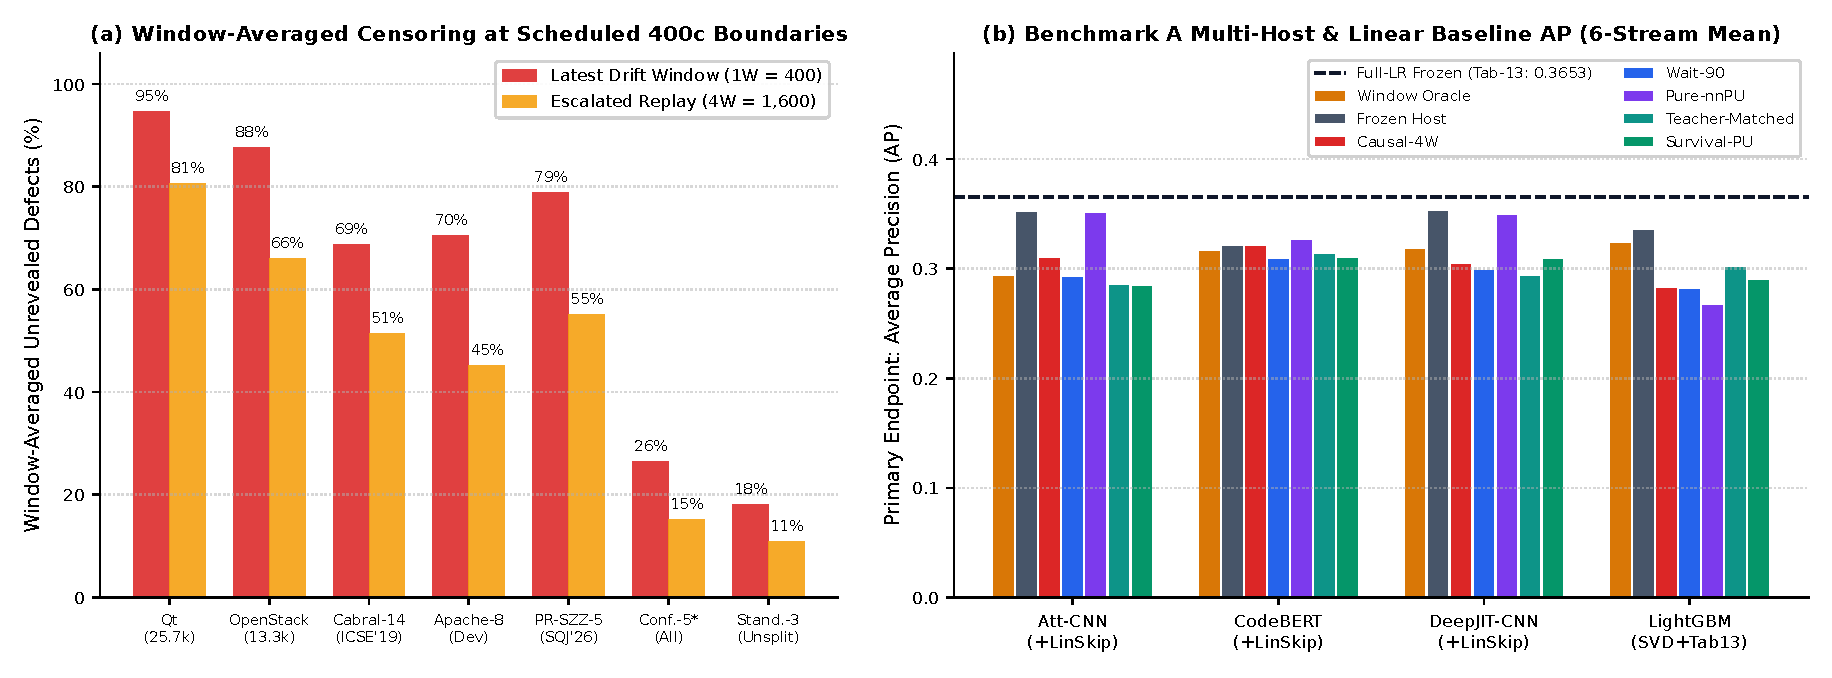
\includegraphics[width=0.98\textwidth]{fig1_multimodal_audit_v3.pdf}
  \caption{(a) Window-averaged fraction of unrevealed true defects across scheduled $400$-commit ($1W$) and $1{,}600$-commit ($4W$) stream boundaries (RQ1). (b) Six-stream mean AP across all four Benchmark~A host families (+frozen linear skip on neural hosts) relative to frozen tabular \texttt{Full-LR} ($0.3653$), bridging directly into RQ2.}
  \label{fig:rq1_overview}
\end{figure}

\textbf{Severe Right-Censoring Across Multi-Year Cohorts.} Cohort-level averages reveal substantial right-censoring across multi-year software ecosystems, with considerable variation between individual repositories. Table~\ref{tab:audit_censoring} and Figure~\ref{fig:rq1_overview}(a) distinguish two complementary censoring estimands: (i) mean per-window unrevealed defect proportions across all scheduled $400$-commit ($1W$) and $1{,}600$-commit ($4W$) stream boundaries, and (ii) seed-42 fired-alarm $1W$ censoring rates. Across multi-year ecosystems, median SZZ fix latency spans $106.5$ to $275.0$ days. Consequently, across scheduled $1W$ boundaries, \textbf{94.6\%} of window defects in natural Qt (pooled: $95.3\%$ across $981$ window-defects; $95.7\%$ across 20 LightGBM alarms and $100.0\%$ at CodeBERT's alarm), \textbf{87.5\%} in natural OpenStack ($84.4\%$ at LightGBM's alarm), \textbf{68.8\%} across Cabral's 14 streams ($68.2\%$ across 102 seed-42 MLP alarms), \textbf{70.4\%} across ApacheJIT's eight development streams ($65.8\%$ across 40 alarms), and \textbf{78.8\%} across Bludau and Pretschner's five PR-SZZ streams ($78.9\%$ across 23 alarms) remain unfixed. Even across escalated $4W$ windows, $45.1\%$ to $80.5\%$ of defects remain unrevealed in these multi-year cohorts, whereas the slower-cadence, shorter confirmatory ApacheJIT repositories exhibit markedly lower censoring ($26.4\%$ scheduled $1W$, $26.7\%$ at alarms, and $15.2\%$ at $4W$ across all five repositories; and even lower on unsplit Standalone-3: $18.0\%$ scheduled $1W$, $17.4\%$ at alarms, and $10.9\%$ at $4W$).

\textbf{Matched Hindsight Optimism vs.\ Gradual Ranking Retention.} How strongly does leaking those future SZZ fixes into alarm-triggered updates inflate apparent accuracy? Comparing offline window-oracle retraining ($B_{1b}^*$) against strictly matched causal four-window retraining ($B_2\text{-4W}$) across $K=25$ natural donor clusters (full breakdowns in Section~\ref{sec:rq2}, Tables~\ref{tab:bench_b_clusters}--\ref{tab:bench_b_holm}) reveals statistically significant hindsight optimism on both neural and tree hosts. On MLP, $B_{1b}^*$ reaches $0.5241$ AP versus $0.5004$ for $B_2\text{-4W}$ ($\Delta\text{AP} = +0.0237$, 20/0/5 wins, $p_{\text{Holm}} = 6.63 \times 10^{-5}$, $d_z = 0.906$), dropping further to $0.4704$ under single-window $B_2\text{-1W}$. On LightGBM, the hindsight gap widens to $+4.76$ AP points: $B_{1b}^*$ reaches $0.5409$ AP versus $0.4933$ for $B_2\text{-4W}$ ($\Delta\text{AP} = +0.0476$, 23/0/2 wins, $p_{\text{Holm}} = 3.70 \times 10^{-5}$, $d_z = 0.986$; $0.4529$ for $B_2\text{-1W}$).

\textbf{Why Censoring Hurts Differently Across Metrics and Drift Regimes.} Crucially, this hindsight gap does not mean that naive causal replay always fails catastrophically. Consistent with Proposition~\ref{prop:bias}(1), older commits inside a $4W$ replay buffer supply partial reveal maturity, allowing $B_2\text{-4W}$ to improve full-stream MLP AP over frozen $B_0$ on both gradual natural clusters ($0.5004$ vs.\ $0.4566$, $p_{\text{Holm}} = 0.0041$) and controlled abrupt shifts ($0.5578$ vs.\ $0.5064$ post-onset AP), while remaining below matched oracle updates ($B_{1b}^* = 0.5241$ natural; $0.6137$ shifts). The penalty manifests sharply along two other axes predicted by Proposition~\ref{prop:bias}: fixed-$0.5$ thresholded $F_1$ collapses on multimodal Benchmark~A ($0.1650$ for $B_2\text{-4W}$ and $0.1070$ for $B_2\text{-1W}$, compared with $0.2907$ for $\text{Survival-PU}$), and single-window $B_2\text{-1W}$ falls below frozen $B_0$ on the controlled abrupt shifts ($0.5011$ vs.\ $0.5064$ post-onset AP). Having established both the prevalence of right-censoring and the magnitude of hindsight optimism, we turn in RQ2 to evaluating whether maturity-calibrated PU adaptation closes this gap across hosts, ecosystems, and an untouched confirmatory cohort---and where simpler baselines prevail (previewed in Figure~\ref{fig:rq1_overview}(b)).

\rqbox{Summary for RQ1}{Across scheduled $400$-commit boundaries in multi-year cohorts, 68.8\%--94.6\% of window defects are right-censored ($65.8\%\text{--}95.7\%$ at fired alarms). Offline window-oracle supervision significantly inflates AP over matched causal $B_2\text{-4W}$ across $K=25$ donor clusters on both MLP ($+0.0237$, $p_{\text{Holm}} = 6.63\times 10^{-5}$) and LightGBM ($+0.0476$, $p_{\text{Holm}} = 3.70\times 10^{-5}$). Causal $B_2\text{-4W}$ improves AP over frozen $B_0$ on both natural streams and controlled shifts, yet remains below matched oracle updates ($B_{1b}^*$) and loses fixed-$0.5$ thresholded $F_1$; single-window $B_2\text{-1W}$ falls below $B_0$ on the controlled shifts.}

% ----------------------------------------------------------------------------
% 6.2 RQ2
% ----------------------------------------------------------------------------
\subsection{RQ2: Multi-Host, Cross-Project, and Confirmatory Operating Boundaries}
\label{sec:rq2}

\begin{figure}[!htb]
  \centering
  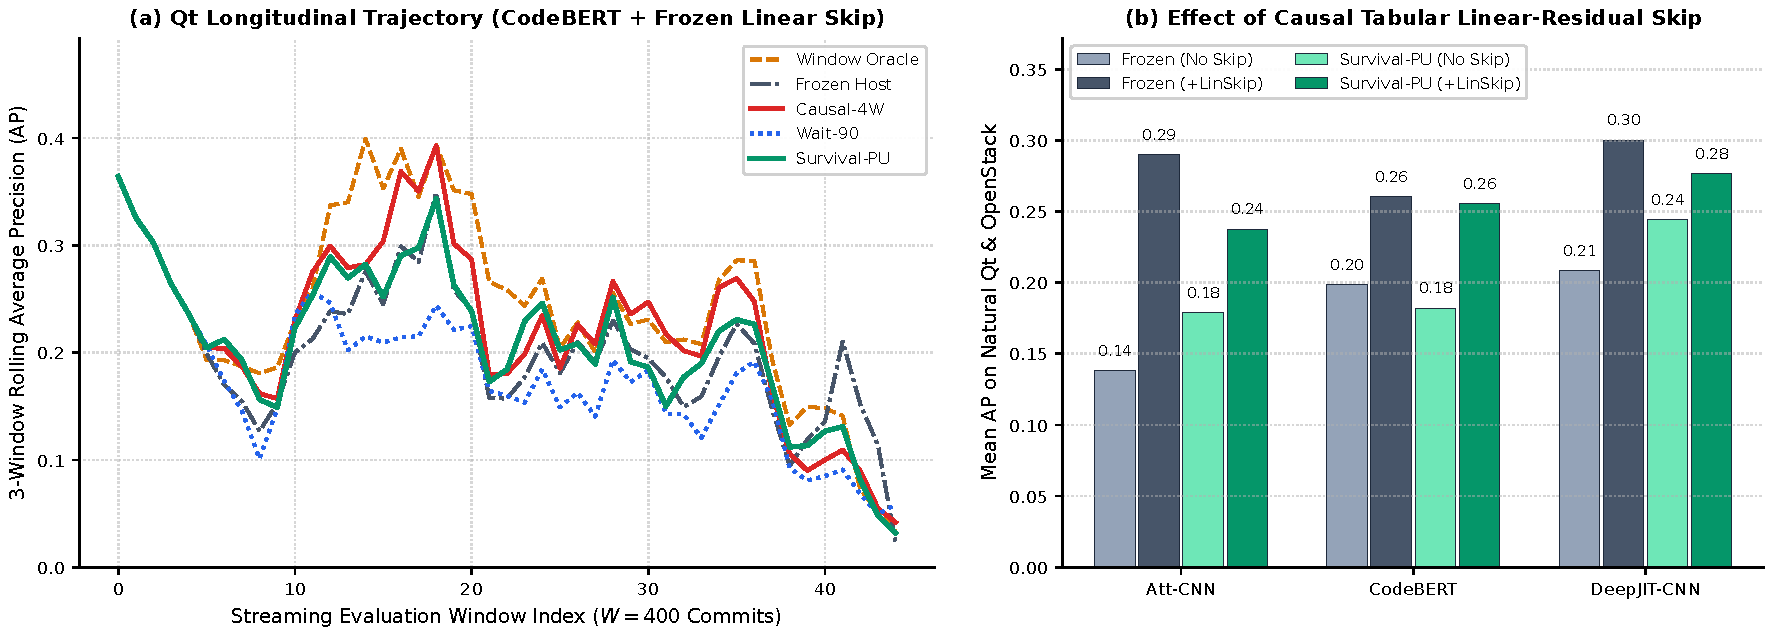
\includegraphics[width=0.98\textwidth]{fig2_trajectories_and_skip_v3.pdf}
  \caption{(a) Prequential 3-window rolling AP trajectory on natural Qt (CodeBERT + frozen linear skip). (b) Effect of adding the causal tabular linear-residual skip connection (no skip vs.\ dev-selected frozen linear skip) on natural Qt and OpenStack.}
  \label{fig:rq2_skip}
\end{figure}

\begin{table}[!htb]
\centering
\caption{Benchmark A causal supervision audit across four multimodal/tree host families (Track 1) and simple/online tabular baselines (Track 2) over six Qt/OpenStack streams (5 seeds; 13 commit-time tabular metrics + code diff/message; frozen linear-residual skip on neural hosts). Bold marks the best deployable value per column.}
\label{tab:bench_a_main}
\fontsize{5.4}{6.8}\selectfont
\setlength{\tabcolsep}{0.8pt}
\begin{tabular*}{\textwidth}{@{\extracolsep\fill}lccccccccc@{}}
\toprule
\textbf{Method} & \textbf{Att.} & \textbf{CodeB.} & \textbf{DJIT} & \textbf{LGBM} & \textbf{AP} & \textbf{$F_1$} & \textbf{$F_{1\mathrm{t}}$} & \textbf{R@20} & \textbf{Brier} \\
\midrule
B1b* (4W Oracle) & 0.2936 & 0.3170 & 0.3188 & 0.3241 & 0.3134 & 0.2937 & 0.3105 & 0.6201 & 0.1265 \\
\midrule
B0 (Frozen) & \textbf{0.3525} & 0.3208 & \textbf{0.3531} & \textbf{0.3356} & 0.3405 & 0.1342 & 0.2565 & 0.6374 & 0.1145 \\
B2-1W (Censored) & 0.3382 & \textbf{0.3268} & 0.3173 & 0.2527 & 0.3087 & 0.1070 & 0.2388 & 0.6044 & 0.1182 \\
B2-4W (Censored) & 0.3098 & 0.3210 & 0.3043 & 0.2824 & 0.3044 & 0.1650 & 0.2788 & 0.6132 & 0.1187 \\
Wait-90 & 0.2932 & 0.3096 & 0.2990 & 0.2816 & 0.2959 & 0.2287 & 0.2865 & 0.6091 & 0.1227 \\
Pure-nnPU & 0.3508 & 0.3263 & 0.3491 & 0.2673 & 0.3234 & 0.0919 & 0.2291 & 0.6222 & 0.1164 \\
FixedCurve-PU (90d) & 0.2948 & 0.3104 & 0.3115 & 0.2908 & 0.3019 & 0.2645 & 0.2987 & 0.6148 & 0.1218 \\
Teacher-Only (Matched) & 0.2859 & 0.3139 & 0.2938 & 0.3024 & 0.2990 & 0.2301 & 0.2892 & 0.6115 & 0.1225 \\
Survival-PU (+Legacy Gate) & 0.2848 & 0.3093 & 0.3071 & 0.2938 & 0.2988 & 0.2878 & 0.3027 & 0.6158 & 0.1251 \\
Survival-PU & 0.2845 & 0.3098 & 0.3097 & 0.2898 & 0.2984 & 0.2907 & 0.3043 & 0.6156 & 0.1251 \\
\midrule
Full-LR Frozen (Track 2) & -- & -- & -- & -- & \textbf{0.3653} & \textbf{0.3939} & \textbf{0.3951} & \textbf{0.6728} & 0.1106 \\
LApredict Frozen (Track 2) & -- & -- & -- & -- & 0.3601 & 0.3853 & 0.3773 & 0.6649 & \textbf{0.1105} \\
Churn-LR Frozen (Track 2) & -- & -- & -- & -- & 0.3397 & 0.3736 & 0.3609 & 0.6520 & 0.1116 \\
BORB ElasticNet (Track 2) & -- & -- & -- & -- & 0.3338 & 0.3525 & 0.3646 & 0.6643 & 0.1125 \\
ORB Hoeffding (Track 2) & -- & -- & -- & -- & 0.2899 & 0.3470 & 0.3466 & 0.6602 & 0.1149 \\
ODaSC Hoeffding (Track 2) & -- & -- & -- & -- & 0.2426 & 0.2389 & 0.3209 & 0.6616 & 0.1167 \\
LOC-Only (Track 2) & -- & -- & -- & -- & 0.0794 & 0.0639 & 0.0639 & 0.6520 & 0.4207 \\
\bottomrule
\end{tabular*}
\end{table}

\begin{table}[!htb]
\centering
\caption{Benchmark A provenance and feature-scope sensitivity evaluated strictly on identical common evaluation commit IDs per ecosystem (CodeBERT + frozen linear skip, AP). Bold marks the highest deployable AP in each row.}
\label{tab:bench_a_sens}
\fontsize{6.2}{7.6}\selectfont
\setlength{\tabcolsep}{1.3pt}
\begin{tabular*}{\textwidth}{@{\extracolsep\fill}lccccc@{}}
\toprule
\textbf{Sensitivity Variant} & \textbf{B0} & \textbf{B1b*} & \textbf{B2-4W} & \textbf{Wait-90} & \textbf{Survival-PU} \\
\midrule
Qt Pre-Merge 28 (CodeBERT) & 0.1472 & 0.1475 & \textbf{0.1603} & 0.1426 & 0.1446 \\
Qt Tier-1 SZZ Only (CodeBERT) & 0.1583 & 0.1791 & \textbf{0.1720} & 0.1550 & 0.1650 \\
Qt Drop Unlinked (CodeBERT) & 0.1654 & 0.1633 & \textbf{0.1912} & 0.1436 & 0.1479 \\
OpenStack Pre-Merge 28 (CodeBERT) & \textbf{0.3332} & 0.2914 & 0.3024 & 0.2934 & 0.2894 \\
OpenStack Tier-1 SZZ Only (CodeBERT) & \textbf{0.3571} & 0.3191 & 0.3285 & 0.3180 & 0.3191 \\
OpenStack Drop Unlinked (CodeBERT) & \textbf{0.3530} & 0.3498 & 0.3408 & 0.3429 & 0.3428 \\
\bottomrule
\end{tabular*}
\end{table}

\textbf{Benchmark A: Simple Linear Predictors Lead Deployable Multimodal Hosts.} Evaluating Track~2 simple baselines alongside all four Track~1 multimodal and tree hosts (Table~\ref{tab:bench_a_main}, Figure~\ref{fig:rq1_overview}(b)) reveals a striking operating boundary on commit-time Qt and OpenStack streams. Across the six Benchmark~A streams, frozen 13-metric logistic regression (\textbf{Full-LR Frozen: $0.3653$ AP, $0.3939$ $F_1$, $0.3951$ $F_{1,\text{th}}$, $0.6728$ R@20\%, $0.1106$ $\text{Brier}_{\text{cal}}$}) and single-feature \textbf{LApredict Frozen} ($0.3601$ AP, $0.3853$ $F_1$, $0.1105$ $\text{Brier}_{\text{cal}}$) outperform \textit{every deployable single-host configuration} (best deployable individual hosts: frozen \texttt{DeepJIT-CNN} $B_0 = 0.3531$, frozen \texttt{Att-CNN} $B_0 = 0.3525$, frozen \texttt{LightGBM} $B_0 = 0.3356$, and \texttt{CodeBERT} $B_2\text{-1W} = 0.3268$ / $B_0 = 0.3208$), as well as the 4-host window-oracle $B_{1b}^*$ ($0.3134$ AP) and full-prefix hindsight $B_{1a}^*$ ($0.3468$ AP) means. Only non-deployable single-host full-prefix hindsight \texttt{DeepJIT-CNN} $B_{1a}^*$ ($0.3768$) exceeds \texttt{Full-LR Frozen}. Meanwhile, \textbf{Churn-LR Frozen} ($0.3397$ AP, $0.3736$ $F_1$) exceeds all window-adapted 4-host means ($0.2959\text{--}0.3234$, spanning $\text{Wait-}90 = 0.2959$ through $\text{Pure-nnPU} = 0.3234$, including $B_{1b}^* = 0.3134$) while trailing frozen \texttt{DeepJIT-CNN} ($0.3531$), \texttt{Att-CNN} ($0.3525$), and the 4-host $B_0$ mean ($0.3405$), and trivial $\text{LOC-Only}$ reaches $0.6520$ R@20\%Effort (exceeding $\text{Survival-PU}$'s $0.6156$).

Adding our causal tabular linear-residual skip substantially narrows the encoder deficit: on the two natural streams plotted in Figure~\ref{fig:rq2_skip}(b), it lifts $B_0$ AP from $0.1379 \to 0.2898$ (Att-CNN), $0.1984 \to 0.2604$ (CodeBERT), and $0.2084 \to 0.3000$ (DeepJIT-CNN)---and across all six Benchmark~A streams from $0.1849 \to 0.3525$, $0.2447 \to 0.3208$, and $0.2697 \to 0.3531$. Even with this architectural boost, however, periodic fine-tuning of high-capacity multimodal encoders on small drift windows still trails frozen linear models in AP. Restricted strictly to identical Track~1 host architectures, base-rate drift and censoring erode fixed-$0.5$ $F_1$ on $B_0$ ($0.1342$) and $B_2\text{-4W}$ ($0.1650$), whereas $\text{Survival-PU}$ recovers the highest Track-1 deployable $F_1$ ($0.2907$, close to $B_{1b}^* = 0.2937$) and $F_{1,\text{th}}$ ($0.3043$) at lower 4-host mean AP ($0.2984$ vs.\ $0.3405$ for $B_0$). Across the feature and SZZ-provenance sensitivity variants in Table~\ref{tab:bench_a_sens} (evaluated on identical common commit IDs: $N=18{,}191$ on Qt and $N=3{,}699$ on OpenStack), $B_2\text{-4W}$ attains the top deployable AP across the three Qt variants ($0.1603\text{--}0.1912$) while frozen $B_0$ leads the three OpenStack variants ($0.3332\text{--}0.3571$). Restricting saved seed-42 predictions to commits with $\ge 180\text{d}$ or $\ge 365\text{d}$ before the archive-horizon proxy $T_{\text{end}}$ (Appendix Table~\ref{tab:followup_sensitivity}) leaves the main conclusions intact---\texttt{Full-LR} retains its AP lead across all six reported slices and \texttt{Survival-PU} retains its Track-1 $F_1$ recovery over $B_2\text{-4W}$ and $B_0$ (also edging \texttt{Full-LR} on Qt $F_1$)---whereas some pairwise AP rankings shift under restriction (e.g., \texttt{Survival-PU} overtakes $B_2\text{-4W}$ and $\text{Wait-}90$ on OpenStack $\ge 365\text{d}$ AP, and $B_0$ overtakes $B_{1b}^*$ on Qt $\ge 365\text{d}$ AP).

\begin{figure}[!htb]
  \centering
  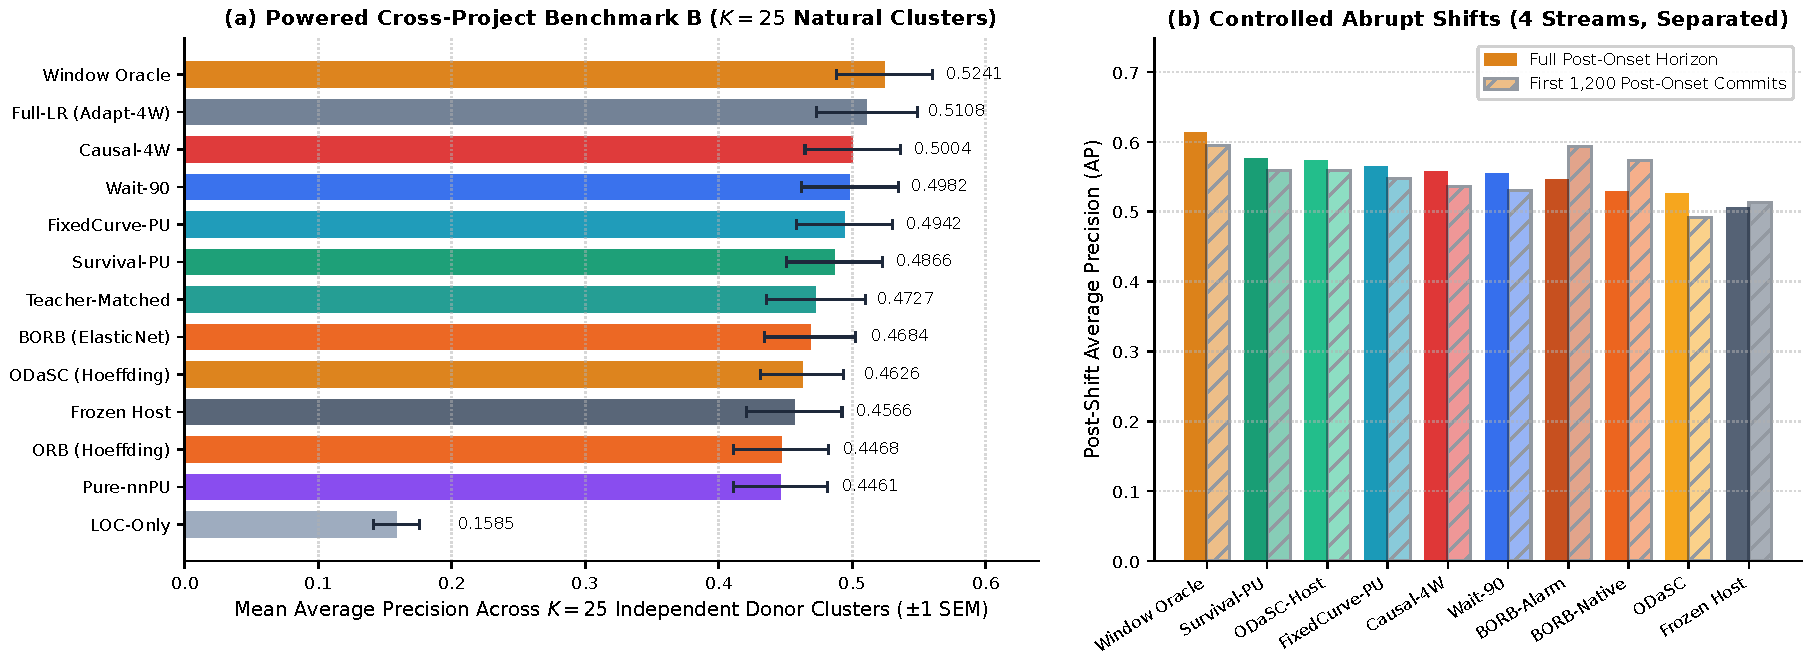
\includegraphics[width=0.98\textwidth]{fig3_benchmark_b_clusters_v3.pdf}
  \caption{(a) Mean AP ($\pm 1$ SEM) across $K=25$ independent natural donor clusters in Benchmark~B. (b) Post-shift AP across the four separated controlled concatenated-shift streams on both full post-onset and first 1,200 post-onset commit horizons.}
  \label{fig:rq2_bench_b}
\end{figure}

\begin{table}[!htb]
\centering
\caption{Benchmark B evaluation across $K=25$ independent natural donor clusters ($K=24$ Benchmark-A-disjoint sensitivity), LightGBM tree host ($K=25$), and separated controlled shift streams (full post-onset AP). Bold marks the best deployable value per column (ties at displayed precision bolded equally).}
\label{tab:bench_b_clusters}
\fontsize{6.2}{7.6}\selectfont
\setlength{\tabcolsep}{1.3pt}
\begin{tabular*}{\textwidth}{@{\extracolsep\fill}lccccccc@{}}
\toprule
\textbf{Method} & \textbf{AP ($K{=}25$)} & \textbf{AP ($K{=}24$)} & \textbf{$F_{1,\mathrm{th}}$} & \textbf{AUC} & \textbf{Brier$\downarrow$} & \textbf{LGB ($K{=}25$)} & \textbf{Shift AP} \\
\midrule
B1b* (4W Oracle) & 0.5241 & 0.5237 & 0.4935 & 0.7803 & 0.1517 & 0.5409 & 0.6137 \\
\midrule
B0 (Frozen) & 0.4566 & 0.4553 & 0.3725 & 0.7363 & 0.1662 & 0.4628 & 0.5064 \\
B2-1W (Censored) & 0.4704 & 0.4689 & 0.4146 & 0.7375 & 0.1658 & 0.4529 & 0.5011 \\
B2-4W (Censored) & 0.5004 & 0.4999 & 0.4638 & 0.7645 & 0.1568 & \textbf{0.4933} & 0.5578 \\
Wait-90 & 0.4982 & 0.4980 & 0.4734 & 0.7634 & 0.1548 & 0.4425 & 0.5554 \\
Pure-nnPU & 0.4461 & 0.4443 & 0.3621 & 0.7107 & 0.1649 & 0.4615 & 0.5017 \\
ODaSC-Host (Track 1) & 0.4949 & 0.4944 & 0.4740 & 0.7621 & 0.1540 & -- & 0.5727 \\
FixedCurve-PU (90d) & 0.4942 & 0.4946 & 0.4782 & 0.7643 & \textbf{0.1525} & 0.4680 & 0.5652 \\
Teacher-Only (Exact) & 0.4802 & 0.4791 & 0.4684 & 0.7560 & 0.1567 & 0.4186 & 0.5461 \\
Teacher-Only (Matched) & 0.4727 & 0.4711 & 0.4659 & 0.7524 & 0.1587 & 0.4240 & 0.5330 \\
Survival-PU (+Legacy Gate) & 0.4873 & 0.4870 & 0.4778 & 0.7602 & 0.1531 & -- & 0.5717 \\
Survival-PU & 0.4866 & 0.4867 & 0.4795 & 0.7593 & \textbf{0.1525} & 0.4619 & \textbf{0.5764} \\
\midrule
LOC-Only (Track 2) & 0.1585 & 0.1610 & 0.1153 & 0.2245 & 0.4721 & -- & 0.2047 \\
LApredict Frozen (Track 2) & 0.4684 & 0.4643 & 0.4416 & 0.7571 & 0.1585 & -- & 0.5529 \\
Full-LR Adapt-4W (Track 2) & \textbf{0.5108} & \textbf{0.5108} & 0.4781 & \textbf{0.7749} & 0.1531 & -- & 0.5469 \\
BORB ElasticNet (Track 2) & 0.4684 & 0.4663 & \textbf{0.5144} & 0.7463 & 0.1617 & -- & 0.5292 \\
BORB-Alarm ElasticNet (Track 2) & 0.4800 & 0.4777 & 0.4912 & 0.7540 & 0.1611 & -- & 0.5461 \\
ORB Hoeffding (Track 2) & 0.4468 & 0.4446 & 0.4736 & 0.7461 & 0.1734 & -- & 0.4928 \\
ODaSC Hoeffding (Track 2) & 0.4626 & 0.4618 & 0.4951 & 0.7564 & 0.1702 & -- & 0.5257 \\
\bottomrule
\end{tabular*}
\end{table}

\begin{table}[!htb]
\centering
\caption{Protocol-specified paired cluster-level Wilcoxon signed-rank inference with Holm--Bonferroni multiplicity adjustment across $K=25$ independent natural donor clusters (primary endpoint: whole-stream AP). Bold indicates $p_{\mathrm{Holm}} < 0.05$ (note the sign of $\Delta\mathrm{AP} = \mathrm{AP}(A) - \mathrm{AP}(B)$).}
\label{tab:bench_b_holm}
\fontsize{6.0}{7.3}\selectfont
\setlength{\tabcolsep}{1.2pt}
\begin{tabular*}{\textwidth}{@{\extracolsep\fill}lcccc@{}}
\toprule
\textbf{Protocol-Specified Contrast ($A$ vs.\ $B$)} & \textbf{$\Delta\mathrm{AP}$ [95\% CI]} & \textbf{W/T/L} & \textbf{$d_z$} & \textbf{$p_{\mathrm{Holm}}$} \\
\midrule
(F1) B1b* (4W Oracle) vs. B2-4W (Censored) & \textbf{+0.0237} [0.0146, 0.0345] & 20/0/5 & 0.906 & \textbf{6.63e-05} \\
(F1) B0 (Frozen) vs. B2-4W (Censored) & \textbf{-0.0438} [-0.0761, -0.0176] & 6/0/19 & -0.568 & \textbf{0.0041} \\
(F1) Survival-PU vs. B2-4W (Censored) & \textbf{-0.0138} [-0.0241, -0.0052] & 7/0/18 & -0.554 & \textbf{0.0056} \\
\midrule
(F2) Survival-PU vs. B0 (Frozen) & +0.0299 [0.0015, 0.0650] & 16/0/9 & 0.359 & 0.2673 \\
(F2) Survival-PU vs. Wait-90 & \textbf{-0.0117} [-0.0222, -0.0008] & 5/0/20 & -0.426 & \textbf{0.0069} \\
(F2) Survival-PU vs. Pure-nnPU & \textbf{+0.0405} [0.0185, 0.0704] & 18/0/7 & 0.593 & \textbf{0.0020} \\
(F2) Survival-PU vs. Full-LR (Adapt-4W) & -0.0243 [-0.0413, -0.0082] & 9/0/16 & -0.560 & 0.0639 \\
(F2) Survival-PU vs. BORB (ElasticNet) & +0.0181 [-0.0069, 0.0433] & 14/0/11 & 0.275 & 0.2673 \\
(F2) Survival-PU vs. ORB (Hoeffding) & \textbf{+0.0398} [0.0147, 0.0663] & 19/0/6 & 0.584 & \textbf{0.0279} \\
(F2) Survival-PU vs. ODaSC (Hoeffding) & +0.0240 [-0.0014, 0.0494] & 19/0/6 & 0.364 & 0.1652 \\
\midrule
(F3) Survival-PU vs. FixedCurve-PU (90d) & \textbf{-0.0077} [-0.0128, -0.0024] & 6/0/19 & -0.569 & \textbf{0.0295} \\
(F3) Survival-PU vs. Teacher-Only (Matched) & +0.0139 [-0.0011, 0.0332] & 12/0/13 & 0.311 & 0.9157 \\
(F3) Survival-PU vs. Teacher-Only (Exact) & +0.0064 [-0.0069, 0.0231] & 13/0/12 & 0.161 & 0.9157 \\
(F3) Survival-PU vs. Survival-PU (+Legacy Gate) & -0.0007 [-0.0028, 0.0015] & 10/0/15 & -0.130 & 0.8988 \\
\bottomrule
\end{tabular*}
\end{table}

\begin{table}[!htb]
\centering
\caption{Evaluation-granularity and cross-window score-comparability diagnostic across $K=25$ natural Benchmark~B clusters (5 seeds $42$--$46$, $531$ operational $400$-commit windows, $0$ excluded; text $p$-values are exploratory unadjusted Pratt Wilcoxon tests distinct from Table~\ref{tab:bench_b_holm}'s $p_{\mathrm{Holm}}$). Bold marks the best deployable value per column.}
\label{tab:window_ap_scale}
\fontsize{5.6}{7.0}\selectfont
\setlength{\tabcolsep}{0.9pt}
\begin{tabular*}{\textwidth}{@{\extracolsep\fill}lccccc@{}}
\toprule
\textbf{Method (5-Seed $K=25$)} & \textbf{Whole AP} & \textbf{Win-AP (Unw.)} & \textbf{Win-AP (Pos-W)} & \textbf{Z-Norm} & \textbf{Rank-Norm} \\
\midrule
B1b* (4W Oracle) & 0.5240 & 0.5473 & 0.5700 & 0.5204 & 0.5254 \\
\midrule
Full-LR Adapt-4W & \textbf{0.5118} & \textbf{0.5270} & \textbf{0.5526} & \textbf{0.5092} & \textbf{0.5097} \\
B2-4W (Censored) & 0.5015 & 0.5192 & 0.5442 & 0.4968 & 0.4989 \\
Wait-90 & 0.4986 & 0.5251 & 0.5489 & 0.5039 & 0.5036 \\
FixedCurve-PU (90d) & 0.4944 & 0.5246 & 0.5489 & 0.5016 & 0.5035 \\
Survival-PU & 0.4863 & 0.5246 & 0.5478 & 0.4990 & 0.5027 \\
B0 (Frozen) & 0.4569 & 0.4664 & 0.4939 & 0.4481 & 0.4494 \\
\bottomrule
\end{tabular*}
\end{table}

\textbf{Benchmark B: Gradual Natural Clusters ($K=25$ Primary AP, Multi-Seed Per-Window AP, Controlled Scale Removal, and Secondary Endpoints).} Tables~\ref{tab:bench_b_clusters}--\ref{tab:window_ap_scale} and Figure~\ref{fig:rq2_bench_b}(a) report our powered cross-project inference across $K=25$ independent natural donor clusters ($K=24$ Benchmark-A-disjoint sensitivity). On primary whole-stream MLP AP, \textbf{Full-LR Adapt-4W} achieves the highest deployable mean ($0.5108$), followed by $B_2\text{-4W}$ ($0.5004$), $\text{Wait-}90$ ($0.4982$), and zero-fit \textbf{FixedCurve-PU} ($0.4942$). Within this landscape, $\text{Survival-PU}$ ($0.4866$) significantly outperforms canonical $\text{Pure-nnPU}$ ($0.4461$, $\Delta\text{AP} = +0.0405$, 18/0/7, $p_{\text{Holm}} = 0.0020$) and Hoeffding $\text{ORB}$ ($0.4468$, $\Delta\text{AP} = +0.0398$, 19/0/6, $p_{\text{Holm}} = 0.0279$), and does not differ significantly after Holm correction from $B_0$ ($0.4566$, $p_{\text{Holm}} = 0.2673$), $\text{ODaSC}$ ($0.4626$, $p_{\text{Holm}} = 0.1652$), ElasticNet $\text{BORB}$ ($0.4684$, $p_{\text{Holm}} = 0.2673$), or $\text{Full-LR Adapt-4W}$ ($0.5108$, $p_{\text{Holm}} = 0.0639$). However, \textbf{$\text{Survival-PU}$ trails $B_2\text{-4W}$ ($\Delta\text{AP} = -0.0138$, $p_{\text{Holm}} = 0.0056$) and $\text{Wait-}90$ ($\Delta\text{AP} = -0.0117$, $p_{\text{Holm}} = 0.0069$) significantly on primary whole-stream AP}.

To test whether this whole-stream deficit reflects weaker within-window discrimination or cross-window score-comparability differences (Proposition~\ref{prop:bias} Remark), Table~\ref{tab:window_ap_scale} evaluates all seven core methods across 5 seeds ($42\text{--}46$) on the exact same $K=25$ clusters ($531$ operational $400$-commit windows; $0$ single-class windows excluded; diagnostic $p$-values below are exploratory and unadjusted per Section~\ref{sec:metrics_protocol}). Moving from whole-stream AP ($B_2\text{-4W} = 0.5015$ vs.\ $\text{Survival-PU} = 0.4863$, $\Delta = -0.0152$, $5/1/19$, $p=0.0024$) to unweighted per-window AP reverses the sign against $B_2\text{-4W}$ into a small non-significant mean advantage (\textbf{$\text{Survival-PU} = 0.5246 > B_2\text{-4W} = 0.5192$}, $\Delta = +0.0054$, 95\% CI $[+0.0009, +0.0101]$, $16/1/8$, $p=0.0569 > 0.05$; positive-weighted Win-AP: $0.5478$ vs.\ $0.5442$, $\Delta = +0.0036$, $17/1/7$, $p=0.0930$), while leaving $\text{Survival-PU}$ numerically close to $\text{FixedCurve-PU}$ ($0.5246$, $p=0.9895$) and $\text{Wait-}90$ ($0.5251$, $p=0.8222$) and slightly behind $\text{Full-LR Adapt-4W}$ ($0.5270$, $p=0.6150$). Applying \textbf{controlled scale removal}---strictly monotone within-window z-score or percentile-rank standardization on the \textit{exact same predictions} before computing concatenated whole-stream AP---reverses $\text{Survival-PU}$'s $-0.0152$ mean whole-stream deficit relative to $B_2\text{-4W}$ under both Z-Norm ($0.4990$ vs.\ $0.4968$, $+0.0023$, $17/1/7$, $p=0.1954$) and Rank-Norm ($0.5027$ vs.\ $0.4989$, $+0.0038$, $16/1/8$, $p=0.0877$). Under Rank-Norm, mean gaps against $\text{FixedCurve-PU}$ ($-0.0008$, $p=0.6244$) and $\text{Wait-}90$ ($-0.0009$, $p=0.9053$) shrink near zero (under Z-Norm, a smaller gap persists vs.\ $\text{Wait-}90$ [$-0.0048$, $p=0.0265$] and $\text{FixedCurve-PU}$ [$-0.0026$, $p=0.2149$]). This cross-window comparability diagnostic supports that inter-window score scaling plays a major role in $\text{Survival-PU}$'s whole-stream deficit vs.\ $B_2\text{-4W}$ (while within-window gains over $B_2\text{-4W}$ remain modest and do not surpass $\text{Wait-}90$, $\text{FixedCurve-PU}$, or $\text{Full-LR}$); because standardization removes inter-window location, scale, and quantile differences jointly, the specific training mechanism generating those shifts is not isolated separately.

Secondary endpoints exhibit a clear metric split. ElasticNet $\text{BORB}$ ($0.5144$) and Hoeffding $\text{ODaSC}$ ($0.4951$) achieve the highest causally tuned $F_{1,\text{th}}$ overall (with $\text{Survival-PU}$ leading Track-1 methods at $0.4795$). On post-Platt Brier loss, $\text{FixedCurve-PU}$ ($0.15247$) and $\text{Survival-PU}$ ($0.15255$) are numerically close at four-decimal display ($0.1525$), ahead of $\text{Full-LR Adapt-4W}$ ($0.1531$) and $B_2\text{-4W}$ ($0.1568$).

\textbf{Benchmark B: Codified Component Controls (Family 3).} Testing whether cohort survival estimation and Stage~3 distillation justify their added complexity reveals important negative and host-dependent findings. On $K=25$ primary AP, \textbf{zero-fit FixedCurve-PU achieved significantly higher AP than cohort-estimated Survival-PU on both MLP ($0.4942$ vs.\ $0.4866$, $\Delta\text{AP} = -0.0077$, 6/0/19, $p_{\text{Holm}} = 0.0295$; $K=24$: $p_{\text{Holm}} = 0.0317$) and LightGBM ($0.4680$ vs.\ $0.4619$, $p_{\text{Holm}} = 0.0367$)}. The specific mechanism behind this difference (e.g., finite-sample survival-curve variance versus parametric prior shape) is not isolated by the benchmark design; quoting our codified decision rule verbatim: ``\textit{An incremental benefit over FixedCurve\_PU was not established on this cohort.}''

Comparing $\text{Survival-PU}$ ($0.4866$) against optimizer-step-matched $\text{Teacher-Only (Matched)}$ ($0.4727$) on $K=25$ MLP similarly yields $p_{\text{Holm}} = 0.9157$ ($K=24$: $p_{\text{Holm}} = 0.9495$); quoting our codified rule verbatim: ``\textit{An incremental benefit over Teacher\_Only\_Matched was not established on this cohort.}'' On the LightGBM host ($K=25$), by contrast, Stage~3 PU distillation delivers a large, significant gain over both $\text{Teacher-Only (Matched)}$ ($0.4619$ vs.\ $0.4240$, $+0.0379$, 19/0/6, $p_{\text{Holm}} = 9.87 \times 10^{-4}$) and $\text{Teacher-Only (Exact)}$ ($0.4186$, $p_{\text{Holm}} = 0.0135$), although causal $B_2\text{-4W}$ achieves the highest deployable $K=25$ LightGBM AP overall ($0.4933$). Finally, an incremental benefit from legacy three-state gating was not established ($\text{Survival-PU (+Legacy Gate)} = 0.4873$ vs.\ $0.4866$, $p_{\text{Holm}} = 0.8988$).

\textbf{Benchmark B: Controlled Concatenated Distribution Shifts Depend on Evaluation Horizon (4 Separated Streams).} Under sharp cross-project or cross-subsystem regime changes (Table~\ref{tab:bench_b_clusters}, rightmost column; Figure~\ref{fig:rq2_bench_b}(b); full per-stream breakdown across all four shifts in Appendix Table~\ref{tab:shift_4streams}), method rankings reverse depending on horizon length. Over the \textbf{full post-onset horizon}, $\text{Survival-PU}$ achieves the highest observed deployable mean AP (\textbf{0.5764}), closely followed by Track-1 $\text{ODaSC-Host}$ ($0.5727$), $B_2\text{-4W-Bal}$ ($0.5708$), $\text{Wait-}30$ ($0.5684$), and $\text{FixedCurve-PU}$ ($0.5652$), whereas single-window $B_2\text{-1W}$ ($0.5011$), age-blind $\text{Pure-nnPU}$ ($0.5017$), and $\text{ORB}$ ($0.4928$) fall below frozen $B_0$ ($0.5064$). Over the \textbf{immediate first 1,200 post-onset commits}, however, ElasticNet batch-oversampling \textbf{BORB-Alarm ($0.5931$)} and \textbf{BORB-Native ($0.5734$)} adapt fastest, surpassing $\text{Survival-PU}$ ($0.5591$), $\text{Wait-}30$ ($0.5587$), and $\text{ODaSC-Host}$ ($0.5586$). Per-stream inspection (Table~\ref{tab:shift_4streams}) also shows substantial stream heterogeneity: the fourth shift stream (\texttt{OS Nova$\to$Neutron}) exhibits lower AP across all adaptive methods ($0.4214$ post-onset / $0.4358$ first-1,200 for $\text{Survival-PU}$) than the three cross-project shifts in RQ4d ($0.4836\text{--}0.6799$).

\begin{figure}[!htb]
  \centering
  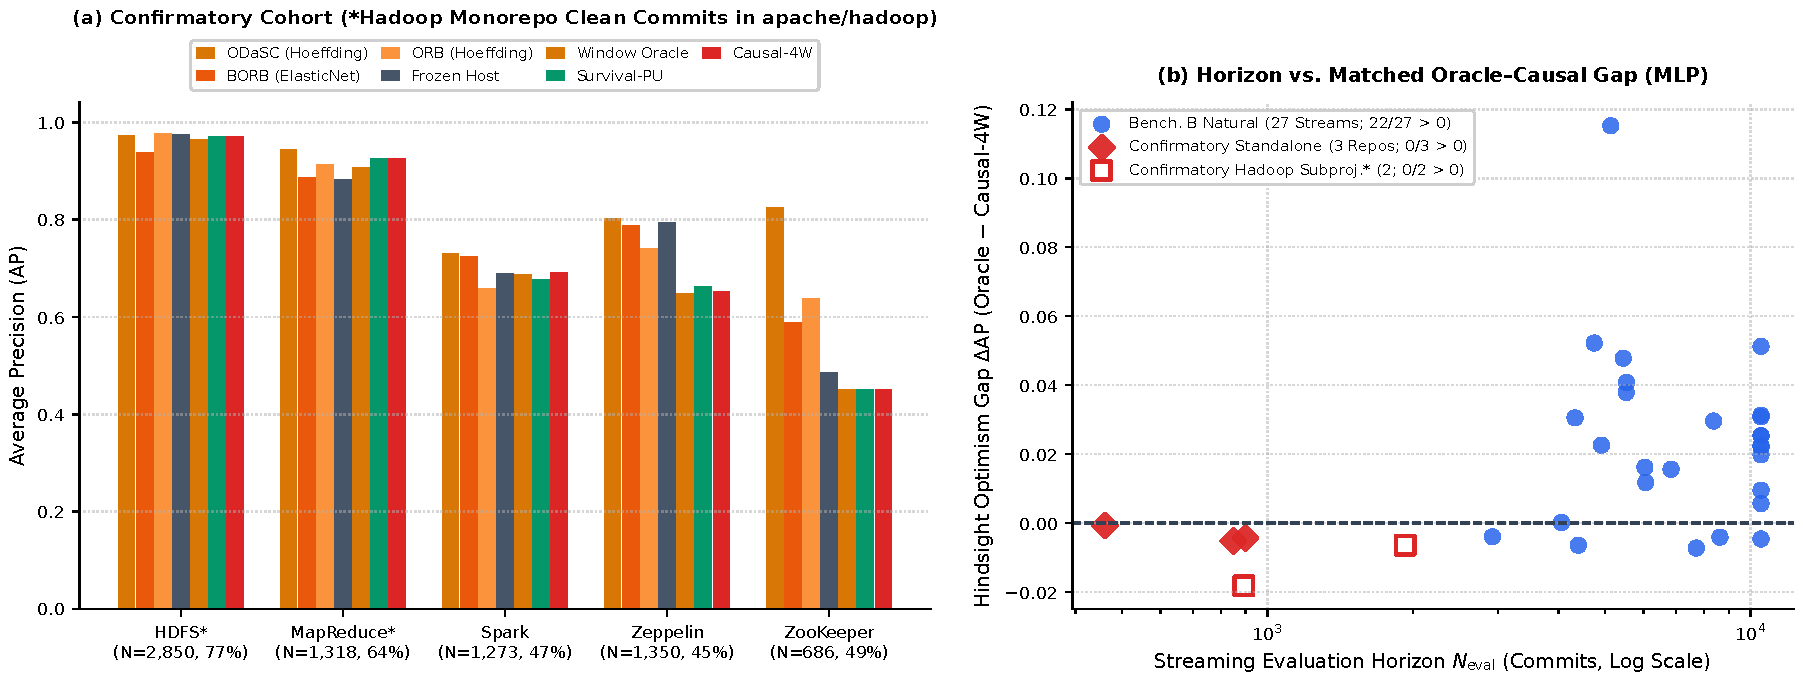
\includegraphics[width=0.98\textwidth]{fig4_confirmatory_boundary_v3.pdf}
  \caption{(a) Out-of-sample AP across the five confirmatory ApacheJIT repositories (asterisks mark Hadoop monorepo subprojects whose clean commits reside in \texttt{apache/hadoop}). (b) Exploratory association plotting evaluation horizon $N_{\text{eval}}$ against the matched oracle-minus-causal hindsight gap $\Delta\text{AP}(B_{1b}^* - B_2\text{-4W})$ on MLP across the 27 natural Benchmark~B streams ($22/27 > 0$) and five confirmatory repositories ($0/5 > 0$, separating Standalone-3 from Hadoop Monorepo-2).}
  \label{fig:rq2_confirmatory}
\end{figure}

\begin{table}[!htb]
\centering
\caption{Out-of-sample evaluation on the untouched confirmatory ApacheJIT cohort ($5$ repositories grouped into $K=4$ umbrella ecosystems; frozen protocol configuration). Asterisks (*) mark Hadoop monorepo subprojects whose clean commits reside under \texttt{apache/hadoop} in upstream \texttt{apachejit\_total.csv} (full funnel and Standalone-3 vs.\ Monorepo-2 split in Table~\ref{tab:confirmatory_funnel}). Bold marks the best deployable AP per column.}
\label{tab:confirmatory}
\fontsize{6.3}{7.8}\selectfont
\setlength{\tabcolsep}{1.4pt}
\begin{tabular*}{\textwidth}{@{\extracolsep\fill}lccccccc@{}}
\toprule
\textbf{Method} & \textbf{HDFS*} & \textbf{MapRed.*} & \textbf{Spark} & \textbf{Zeppelin} & \textbf{ZooKeep.} & \textbf{Umb-4 MLP} & \textbf{Umb-4 LGB} \\
\midrule
ODaSC Hoeffding (Track 2) & 0.9736 & \textbf{0.9438} & \textbf{0.7296} & \textbf{0.8021} & \textbf{0.8253} & \textbf{0.8289} & -- \\
BORB ElasticNet (Track 2) & 0.9378 & 0.8854 & 0.7244 & 0.7878 & 0.5880 & 0.7530 & -- \\
ORB Hoeffding (Track 2) & \textbf{0.9758} & 0.9125 & 0.6582 & 0.7405 & 0.6382 & 0.7453 & -- \\
Full-LR Frozen (Track 2) & 0.9552 & 0.9357 & 0.7130 & 0.7694 & 0.4946 & 0.7306 & -- \\
\midrule
B1a* (Full Hindsight) & 0.9915 & 0.9069 & 0.7385 & 0.6942 & 0.6483 & 0.7575 & -- \\
B0 (Frozen) & 0.9743 & 0.8818 & 0.6897 & 0.7940 & 0.4858 & 0.7244 & 0.7005 \\
B1b* (4W Oracle) & 0.9635 & 0.9070 & 0.6864 & 0.6485 & 0.4504 & 0.6801 & 0.7020 \\
Teacher-Only (Matched) & 0.9729 & 0.9325 & 0.6900 & 0.6642 & 0.4558 & 0.6907 & \textbf{0.7019} \\
B2-4W (Censored) & 0.9700 & 0.9253 & 0.6916 & 0.6529 & 0.4511 & 0.6858 & 0.6976 \\
Survival-PU & 0.9709 & 0.9253 & 0.6768 & 0.6629 & 0.4506 & 0.6846 & 0.6949 \\
FixedCurve-PU (90d) & 0.9704 & 0.9074 & 0.6820 & 0.6629 & 0.4542 & 0.6845 & 0.6884 \\
Wait-90 & 0.9685 & 0.9205 & 0.6868 & 0.6535 & 0.4510 & 0.6840 & 0.6958 \\
\bottomrule
\end{tabular*}
\end{table}

\textbf{Phase C: Confirmatory Non-Replication on MLP — Standalone-3 Primary Interpretation vs.\ Frozen Umbrella-4 Record.} Table~\ref{tab:confirmatory} and Figure~\ref{fig:rq2_confirmatory} report out-of-sample results on the five confirmatory ApacheJIT repositories. Because upstream \texttt{apachejit\_total.csv} omits $11{,}964$ clean Hadoop monorepo commits into \texttt{apache/hadoop} (elevating \texttt{HDFS*} and \texttt{MapReduce*} evaluation prevalence to $89.2\%$ and $78.8\%$; Table~\ref{tab:confirmatory_funnel}), those two slices reflect an archive distribution with class-dependent clean-commit omission rather than natural repository base rates. Accordingly, the \textbf{three standalone repositories} (\texttt{Spark}, \texttt{Zeppelin}, \texttt{ZooKeeper}---a post-audit 3-repo subgroup free of monorepo splitting) provide the cleaner external check: here \textbf{MLP hindsight optimism did not replicate}, with $B_{1b}^*$ ($0.5951$) still trailing $B_2\text{-4W}$ ($0.5985$) and frozen $B_0$ ($0.6565$), while Hoeffding \textbf{ODaSC ($0.7857$)}, ElasticNet \textbf{BORB ($0.7001$)}, and Hoeffding \textbf{ORB ($0.6790$)} outperform all window-retrained MLP variants ($0.5968\text{--}0.6033$); on Standalone-3 LightGBM, $B_0$ ($0.6211$) leads $B_{1b}^*$ ($0.6173$) and $B_2\text{-4W}$ ($0.6121$).

For transparent protocol completeness, the frozen pre-unlock \textbf{umbrella-4 MLP AP} record shows the identical direction: window-oracle $B_{1b}^*$ ($0.6801$) trailed causal $B_2\text{-4W}$ ($0.6858$, $\Delta\text{AP} = -0.0057$, 0/0/4 umbrella wins, exact two-sided $p = 0.125$, $p_{\text{Holm}} = 0.375$) and trailed frozen $B_0$ ($0.7244$, $\Delta\text{AP} = -0.0443$, 1/0/3 umbrella wins: Hadoop $+0.0072$, Spark $-0.0033$, Zeppelin $-0.1455$, ZooKeeper $-0.0354$; exact two-sided $p = 0.375$), while \textbf{ODaSC ($0.8289$)}, \textbf{BORB ($0.7530$)}, and \textbf{ORB ($0.7453$)} led (on LightGBM umbrella-4, $B_{1b}^* = 0.7020$ stayed slightly above $B_2\text{-4W} = 0.6976$, 3/0/1 wins, $p = 0.375$; on the two Hadoop slices alone, MLP clustered at $0.9116\text{--}0.9587$ with $B_{1b}^* = 0.9353 < B_2\text{-4W} = 0.9476$). Because horizon length ($N_{\text{eval}} = 461\text{--}1{,}925$), prevalence, low $1W$ censoring ($18.0\%$ on Standalone-3; $26.4\%$ across all five repositories), alarm count, and project identity covary here, treating ``short, high-prevalence repos favor ODaSC'' as a validated deployment rule would be premature; it remains an exploratory hypothesis.

\rqbox{Summary for RQ2}{Frozen \texttt{Full-LR} ($0.3653$ AP) leads deployable Benchmark~A, while \texttt{Survival-PU} recovers Track-1 $F_1$ ($0.2907$). On $K=25$ whole-stream MLP AP, \texttt{Full-LR Adapt-4W} ($0.5108$, $p_{\text{Holm}}=0.0639$) leads in mean AP while $B_2\text{-4W}$ ($0.5004$, $p_{\text{Holm}}=0.0056$), $\text{Wait-}90$ ($0.4982$, $p_{\text{Holm}}=0.0069$), and \texttt{FixedCurve-PU} ($0.4942$, $p_{\text{Holm}}=0.0295$) significantly exceed \texttt{Survival-PU} ($0.4866$). On 5-seed predictions, within-window standardization reverses the whole-stream mean gap vs.\ $B_2\text{-4W}$ (Rank-Norm: $0.5027$ vs.\ $0.4989$; Z-Norm: $0.4990$ vs.\ $0.4968$), and per-window AP edges $B_2\text{-4W}$ non-significantly ($0.5246$ vs.\ $0.5192$, unadjusted $p=0.0569$) while remaining numerically close to \texttt{Full-LR}, $\text{Wait-}90$, and \texttt{FixedCurve-PU}. \texttt{Survival-PU} leads 4-shift full post-onset AP ($0.5764$), whereas \texttt{BORB-Alarm} leads the first 1,200 commits ($0.5931$). On the confirmatory cohort, MLP hindsight optimism did not replicate on unsplit Standalone-3 ($0.5951$ vs.\ $0.5985$; \texttt{ODaSC} $=0.7857$) or frozen Umbrella-4 ($0.6801$ vs.\ $0.6858$; \texttt{ODaSC} $=0.8289$).}

% ----------------------------------------------------------------------------
% 6.3 RQ3
% ----------------------------------------------------------------------------
\subsection{RQ3: Maturity-Estimator Sensitivity, Mechanism Audit, and Component Ablations}
\label{sec:rq3}

\begin{figure}[!htb]
  \centering
  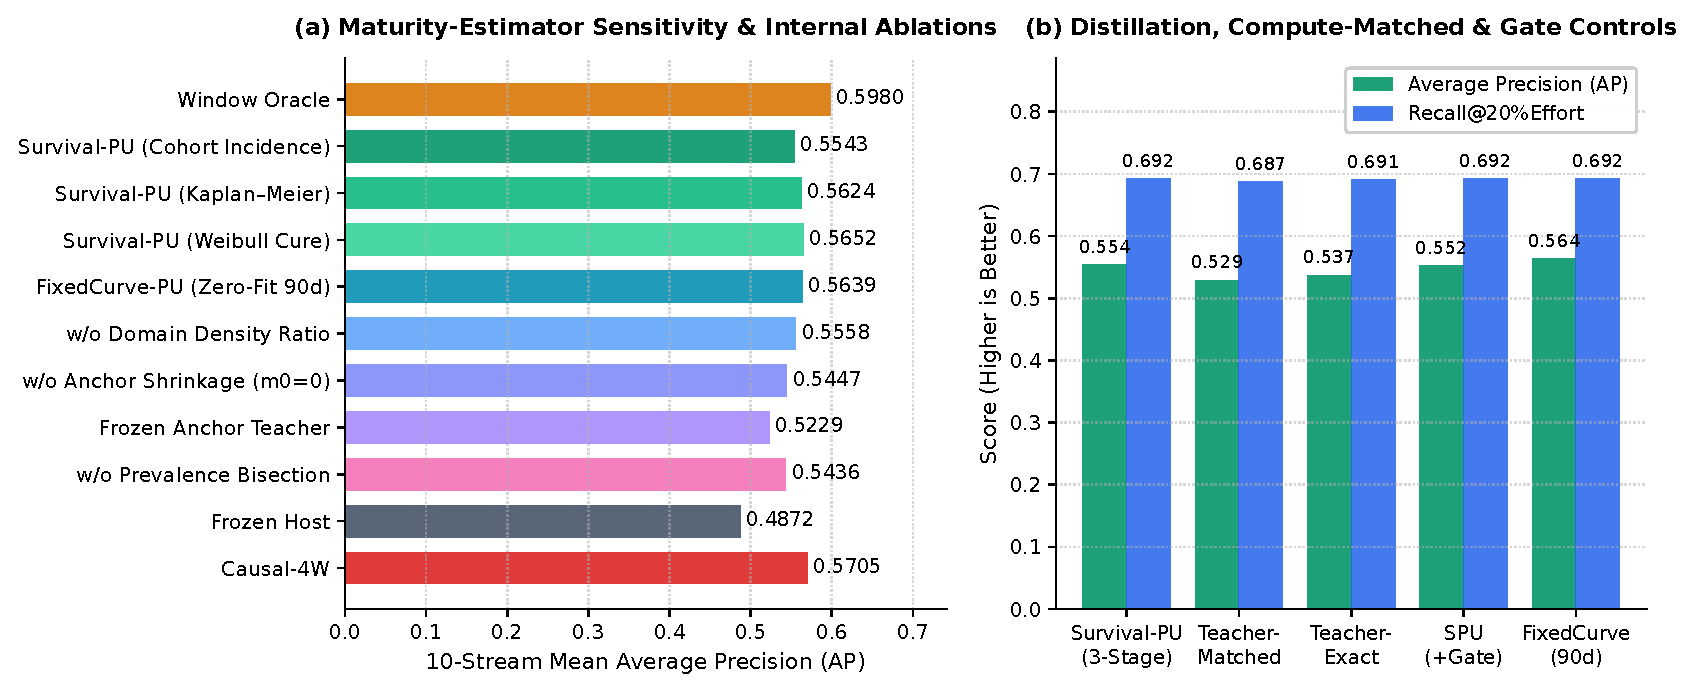
\includegraphics[width=0.98\textwidth]{fig5_ablations_and_controls_v3.pdf}
  \caption{(a) Ten-stream mean AP across three causal maturity estimators, zero-fit \texttt{FixedCurve-PU}, and single-factor internal ablations. (b) Paired AP and Recall@20\%Effort across gate-free Survival-PU, step-matched teacher controls, and legacy three-state gating.}
  \label{fig:rq3_abl}
\end{figure}

\begin{table}[!htb]
\centering
\caption{RQ3 maturity-estimator sensitivity, single-factor component ablations, step-matched teacher controls, and legacy safety-gate ablation across 10 representative streams (5 seeds). Bold marks the best deployable value per column.}
\label{tab:rq3_ablations}
\fontsize{6.4}{7.9}\selectfont
\setlength{\tabcolsep}{1.5pt}
\begin{tabular*}{\textwidth}{@{\extracolsep\fill}lcccccc@{}}
\toprule
\textbf{Variant / Control} & \textbf{AP} & \textbf{$F_{1,\mathrm{th}}$} & \textbf{ROC-AUC} & \textbf{R@20\%Eff} & \textbf{Brier$\downarrow$} & \textbf{Opt.\ Steps} \\
\midrule
B1b* (4W Oracle) & 0.5980 & 0.5541 & 0.7985 & 0.6968 & 0.1658 & 382.2 \\
\midrule
Survival-PU (Default Cohort Incidence) & 0.5543 & 0.5395 & 0.7793 & 0.6920 & \textbf{0.1698} & 869.7 \\
Survival-PU (Kaplan--Meier Cure, $10^{-4}$d) & 0.5624 & \textbf{0.5434} & 0.7826 & 0.6924 & 0.1701 & 868.0 \\
Survival-PU (Weibull Mixture-Cure) & 0.5652 & 0.5389 & \textbf{0.7851} & 0.6913 & 0.1702 & 870.2 \\
FixedCurve-PU (Zero-Fit 90d Half-Life) & 0.5639 & 0.5391 & 0.7850 & 0.6924 & 0.1706 & 870.2 \\
\midrule
w/o Anchor Shrinkage ($m_0 = 0$) & 0.5447 & 0.5347 & 0.7753 & 0.6908 & 0.1725 & 869.7 \\
w/o Monotone Prevalence Bisection & 0.5436 & 0.5330 & 0.7753 & 0.6881 & 0.1747 & 869.7 \\
w/o Covariate Density-Ratio Weighting & 0.5558 & 0.5406 & 0.7797 & \textbf{0.6935} & 0.1704 & 869.7 \\
Frozen Pre-Stream Anchor Teacher & 0.5229 & 0.5233 & 0.7544 & 0.6906 & 0.1745 & 446.8 \\
\midrule
Teacher-Only (Single-Stage Budget) & 0.5371 & 0.5284 & 0.7718 & 0.6912 & 0.1752 & 422.9 \\
Teacher-Only (Step-Matched $2\times$) & 0.5293 & 0.5258 & 0.7677 & 0.6871 & 0.1770 & 869.7 \\
Survival-PU (+Legacy 3-State Gate) & 0.5521 & 0.5374 & 0.7790 & 0.6921 & 0.1704 & 869.7 \\
\midrule
B0 (Frozen) & 0.4872 & 0.4063 & 0.7164 & 0.6515 & 0.1928 & 0.0 \\
B2-4W (Censored) & \textbf{0.5705} & 0.5132 & 0.7802 & 0.6808 & 0.1749 & 382.2 \\
\bottomrule
\end{tabular*}
\end{table}

Table~\ref{tab:rq3_ablations} and Figure~\ref{fig:rq3_abl} dissect maturity-estimator sensitivity and internal component contributions across the ten-stream representative subset (seven independent natural streams plus three controlled cross-project shifts; $K=7$ natural contrasts have exact $p_{\min} = 0.015625 > 0.0125$ and are reported descriptively).

\textbf{Low Sensitivity Across Stage~1 Maturity Estimators.} Replacing risk-eligible cohort cumulative incidence ($0.5543$ AP, $0.5395$ $F_{1,\text{th}}$, $0.6920$ R@20\%Effort) with $10^{-4}$-day Kaplan--Meier cure ($0.5624$ AP, $0.5434$ $F_{1,\text{th}}$), global unstratified Weibull mixture-cure MLE ($0.5652$ AP, $0.5389$ $F_{1,\text{th}}$; a Weibull delay family containing the exponential case at $k=1$, inspired by delayed-feedback/cure likelihoods \citep{chapelle2014modeling}), or zero-fit 90-day $\text{FixedCurve-PU}$ ($0.5639$ AP, $0.5391$ $F_{1,\text{th}}$) spans a narrow descriptive range of $1.09$ AP points and $0.45$ $F_{1,\text{th}}$ points, with zero survival fallbacks and zero unreachable bisection solves across all four variants. On this 10-stream mix, $B_2\text{-4W}$ reaches $0.5705$ AP at lower $F_{1,\text{th}}$ ($0.5132$) and higher $\text{Brier}_{\text{cal}}$ ($0.1749$ vs.\ $0.1698$ for $\text{Survival-PU}$).

\textbf{Unrevealed-Commit Stage~1--3 Mechanism Audit vs.\ FixedCurve-PU and Positive Writeback (Table~\ref{tab:mechanism_audit}).} Because Eq.~\eqref{eq:bayes_pu} sets $q_i = 1$ deterministically on already-revealed positives ($y_{i,\text{obs}}=1$), evaluating all pool commits conflates label writeback with genuine maturity correction on unrevealed commits. Appendix Table~\ref{tab:mechanism_audit} audits all 62 seed-42 DriftLens alarms on the 10 representative streams ($74{,}400$ pool evaluations spanning $59{,}600$ unique commits, comparing \texttt{Survival-PU} and \texttt{FixedCurve-PU} head-to-head). Here retrospective reference maturity $c^*(a) = |\mathcal{P}|^{-1}\sum_{j \in \mathcal{P}} \mathbb{I}(\Delta_j \le a)$ is defined over all archive-labeled positives $\mathcal{P} = \{j : y_j^* = 1\}$ in each stream (counting unlinked $t_j^{\text{fix}} = +\infty$ as unrevealed at every finite age $a$), evaluated on $\mathcal{B}_{\text{cal}}$ commit ages and averaged per alarm before aggregating across alarms ($n=62$) or streams ($n=10$); all $\pm$ dispersion terms in this audit and Table~\ref{tab:mechanism_audit} report sample standard deviations (SD):
\begin{itemize}[leftmargin=1.6em,itemsep=0.06em]
  \item \textit{Stage 1 $\hat{c}(a)$ vs.\ Stage 2 $\hat{\pi}_{\text{target}}$ (Non-Monotonic Cross-Stage Error Propagation):} Adaptive cohort incidence recovers empirical maturity $c^*(a)$ more accurately than the fixed 90-day prior: alarm-level $\hat{c}(a)$ MAE $= 0.0938 \pm 0.0714$ SD (stream-level $0.0873 \pm 0.0403$ SD; $0.0803$ natural vs.\ $0.1257$ shifts) compared with \texttt{FixedCurve-PU}'s $0.1204 \pm 0.0639$ SD (stream-level $0.1310 \pm 0.0594$ SD). Crucially, however, more accurate Stage~1 maturity estimation does \textit{not} automatically yield lower downstream error: on Stage~2 target prevalence, \texttt{FixedCurve-PU} achieves slightly lower alarm-level MAE ($0.0565 \pm 0.0368$ SD) than \texttt{Survival-PU} ($0.0620 \pm 0.0452$ SD, bias $+0.006$, median $n_{\text{eff,heur}} = 125.0$, median anchor weight $28.6\%$; both improve over unshrunk $\hat{\pi}_{\text{IP}} = 0.0712$).
  \item \textit{Disentangling Positive Writeback from Unrevealed-Commit ($y_{\text{obs}}=0$) Soft Targets:} Across all $74{,}400$ pool evaluations ($13.0\%$ observed positives), applying fair positive writeback ($y_{\text{obs}}=1 \to 1.0$) to the de-weighted teacher alone lowers Brier from $0.1525$ to $0.1134$, confirming that writeback accounts for most of the raw all-pool reduction. Restricting strictly to \textbf{unrevealed commits ($y_{\text{obs}} = 0$, $64{,}745$ evaluations, zero writeback)}, soft targets still improve modestly over the de-weighted teacher in every age stratum ($0.1303 \to 0.1236$ for \texttt{Survival-PU}, alarm-level $\Delta = -0.0065 \pm 0.0355$ SD, stream-level $-0.0063 \pm 0.0142$ SD, near-zero bias $+0.0027$). Yet mirroring Stage~2, \texttt{FixedCurve-PU} achieves slightly lower overall unrevealed soft-target Brier ($0.1200$, at negative bias $-0.0358$; lower on young/mid strata while \texttt{Survival-PU} is lower on aged $\ge 90\text{d}$ commits: $0.1181$ vs.\ $0.1194$). This cross-stage trade-off---where better Stage-1 $\hat{c}(a)$ MAE does not translate monotonically into lower Stage-2 prior MAE or Stage-3 unrevealed Brier---is consistent with \texttt{FixedCurve-PU}'s competitiveness on gradual streams, although Brier and signed bias do not directly determine ranking AP and the specific source of \texttt{FixedCurve-PU}'s $K=25$ AP advantage remains unisolated.
\end{itemize}

\textbf{Component Ablations and Simplification Candidates.} Freezing the teacher to the initial pre-stream checkpoint produces the steepest drop ($0.5543 \to 0.5229$ AP, $-3.14$ points), co-occurring with $4.2$ unreachable bisection alarms/stream ($35$ across 5 seeds on \texttt{apache\_flink}, $7$ on \texttt{n60\_airflow}, confounding teacher staleness with clamping). Removing bisection ($0.5436$ AP) or anchor shrinkage $m_0 = 0$ ($0.5447$ AP) degrades both AP and $\text{Brier}_{\text{cal}}$, whereas omitting Stage-2 covariate density ratios slightly improves descriptive AP ($0.5558$ vs.\ $0.5543$), $F_{1,\text{th}}$ ($0.5406$), and R@20\%Eff ($0.6935$) at lower runtime ($8.93\text{ s}$ vs.\ $9.25\text{ s}$), making it an unverified simplification candidate. On this 10-stream subset, \texttt{Survival-PU} ($0.5543$ AP) exceeds step-matched $2\times$ \texttt{Teacher-Only} ($0.5293$) while legacy gating yields $0.5521$.

\rqbox{Summary for RQ3}{Cohort incidence, Kaplan--Meier cure, global Weibull cure, and \texttt{FixedCurve-PU} span $1.09$ AP points with zero fallbacks. Across 62 alarms ($59{,}600$ unique commits; $\pm$ = sample SD), cohort incidence improves Stage-1 $\hat{c}(a)$ MAE over \texttt{FixedCurve-PU} ($0.0938 \pm 0.0714$ vs.\ $0.1204 \pm 0.0639$), yet \texttt{FixedCurve-PU} achieves slightly lower Stage-2 $\hat{\pi}_{\text{target}}$ MAE ($0.0565$ vs.\ $0.0620$) and unrevealed-only ($y_{\text{obs}}=0$) Brier ($0.1200$ vs.\ $0.1236$; both improving over de-weighted teachers at $0.1303$), showing non-monotonic error propagation across stages. Teacher adaptation, bisection, and shrinkage matter most; density-ratio omission ($0.5558$ AP) is a simplification candidate.}

% ----------------------------------------------------------------------------
% 6.4 RQ4
% ----------------------------------------------------------------------------
\subsection{RQ4: Stress Tests Across Latency Extremes, Monitoring, Noise, and Prompting}
\label{sec:rq4}

We subject our findings to five targeted stress tests: future-only latency scaling with symmetrical Raw/Platt and alarm-synchronized post-hoc $B_2$ controls (RQ4a), an unconfounded $2 \times 2$ DriftLens monitoring factorial (RQ4b), independent semi-synthetic PR-SZZ label noise (RQ4c), matched-horizon window and hyperparameter sweeps (RQ4d), and a paired Code-LLM prompting case study (RQ4e).

\begin{figure}[!htb]
  \centering
  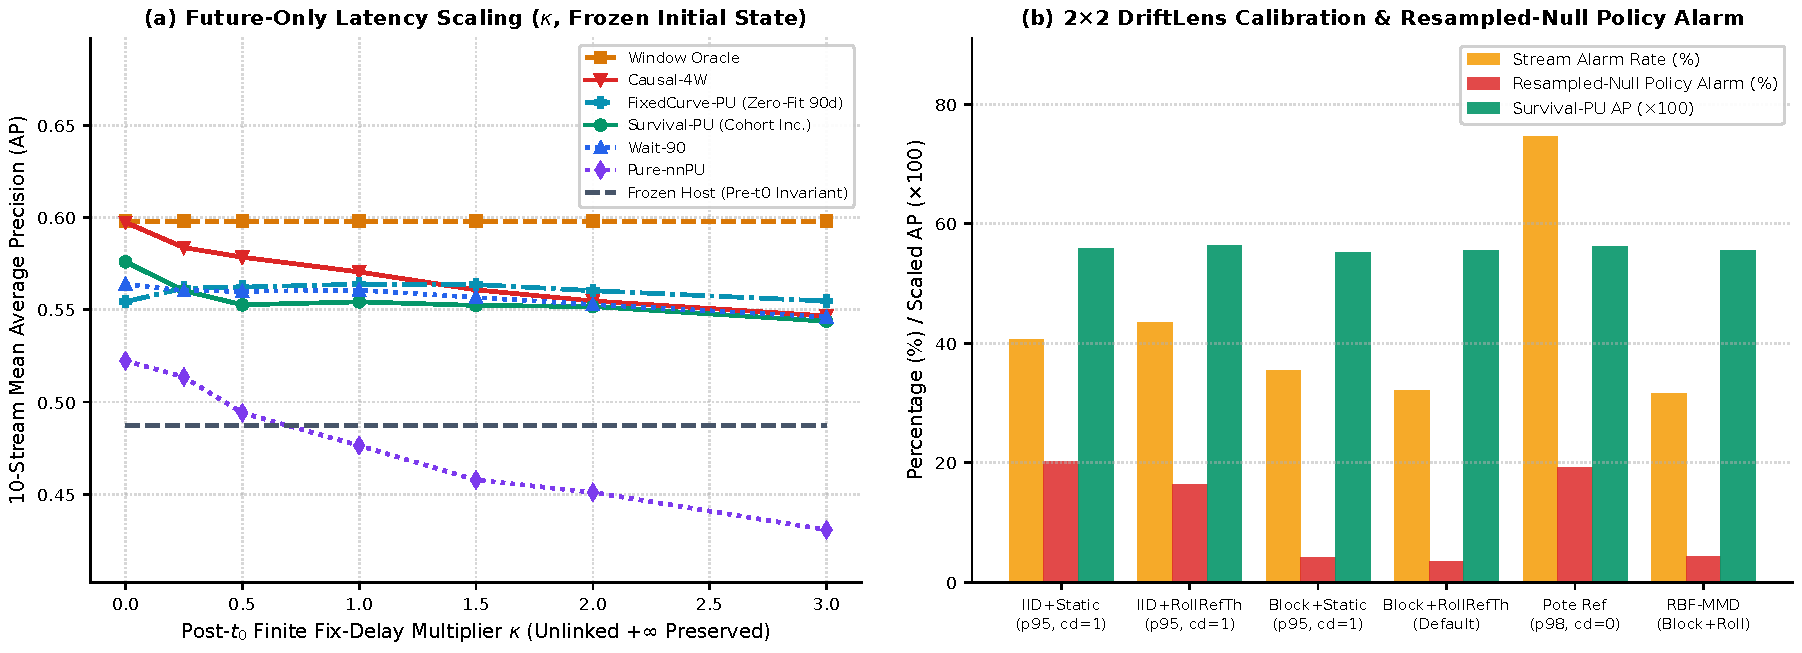
\includegraphics[width=0.98\textwidth]{fig6_latency_and_drift_factorial_v3.pdf}
  \caption{(a) Post-$t_0$ verification-latency scaling ($\kappa \in [0.0, 3.0]$ with frozen pre-$t_0$ supervision, keeping $B_0$ invariant). (b) $2 \times 2$ DriftLens bootstrap/refresh factorial ($p_{95}$, cooldown $1$) plus Pote-inspired reference ($p_{98}$, cooldown $0$) and RBF-MMD.}
  \label{fig:rq4_lat_mon}
\end{figure}

\begin{table}[!htb]
\centering
\caption{RQ4a future-only causal latency scaling across 10 representative streams (5 seeds; pre-$t_0$ supervision frozen so $B_0 = 0.4872$ AP is invariant across all $\kappa$). Bold marks the highest deployable value among the three shown causal baselines (cols 3--5 AP, cols 6--8 $F_1$, cols 9--11 $F_{1,\mathrm{th}}$); the matched zero-fit \texttt{FixedCurve-PU} vs.\ \texttt{Survival-PU} Stage-1 ablation across AP, $F_1$, $F_{1,\mathrm{th}}$, and Brier loss is reported directly in Table~\ref{tab:rq4a_fixedcurve}.}
\label{tab:rq4a_kappa}
\fontsize{5.2}{6.6}\selectfont
\setlength{\tabcolsep}{0.6pt}
\begin{tabular*}{\textwidth}{@{\extracolsep\fill}lcccccccccc@{}}
\toprule
\textbf{Latency Regime} & \textbf{B1b*} & \textbf{B2 AP} & \textbf{W90 AP} & \textbf{SPU AP} & \textbf{B2 $F_1$} & \textbf{W90 $F_1$} & \textbf{SPU $F_1$} & \textbf{B2 $F_{1\mathrm{t}}$} & \textbf{W90 $F_{1\mathrm{t}}$} & \textbf{SPU $F_{1\mathrm{t}}$} \\
\midrule
Oracle Post-$t_0$ ($B_{1b}^* = B_2$) & 0.5980 & 0.5980 & 0.5632 & 0.5763 & 0.5390 & 0.5163 & 0.5357 & 0.5774 & 0.5651 & 0.5666 \\
\midrule
$\kappa = 0.00\times$ (Zero Delay) & 0.5980 & \textbf{0.5974} & 0.5638 & 0.5760 & \textbf{0.5403} & 0.5175 & 0.5364 & \textbf{0.5755} & 0.5634 & 0.5643 \\
$\kappa = 0.25\times$ (Fast Fixes) & 0.5980 & \textbf{0.5837} & 0.5603 & 0.5603 & 0.5264 & 0.5273 & \textbf{0.5353} & 0.5578 & \textbf{0.5609} & 0.5570 \\
$\kappa = 0.50\times$ & 0.5980 & \textbf{0.5785} & 0.5600 & 0.5527 & 0.5093 & 0.5335 & \textbf{0.5363} & 0.5439 & \textbf{0.5520} & 0.5509 \\
$\kappa = 1.00\times$ (Emp.\ SZZ) & 0.5980 & \textbf{0.5705} & 0.5607 & 0.5543 & 0.4687 & 0.5267 & \textbf{0.5377} & 0.5132 & 0.5309 & \textbf{0.5395} \\
$\kappa = 1.50\times$ & 0.5980 & \textbf{0.5608} & 0.5567 & 0.5524 & 0.4361 & 0.5139 & \textbf{0.5339} & 0.4871 & 0.5110 & \textbf{0.5298} \\
$\kappa = 2.00\times$ & 0.5980 & \textbf{0.5548} & 0.5529 & 0.5518 & 0.4137 & 0.5027 & \textbf{0.5348} & 0.4750 & 0.4965 & \textbf{0.5211} \\
$\kappa = 3.00\times$ (Heavy Lat.) & 0.5980 & \textbf{0.5466} & 0.5460 & 0.5438 & 0.3825 & 0.4790 & \textbf{0.5259} & 0.4465 & 0.4736 & \textbf{0.5022} \\
\bottomrule
\end{tabular*}
\end{table}

\begin{table}[!htb]
\centering
\caption{RQ4a Stage-1 maturity-misspecification control: zero-fit 90-day \texttt{FixedCurve-PU} (Fix) vs.\ adaptive cohort-incidence \texttt{Survival-PU} (SPU) across identical future-only latency regimes (10 streams, 5 seeds; exact $0.00$ parity with Table~\ref{tab:rq4a_kappa} on SPU). Bold marks the better of the two Stage-1 estimators per metric (lower is better for post-Platt Brier loss).}
\label{tab:rq4a_fixedcurve}
\fontsize{6.0}{7.4}\selectfont
\setlength{\tabcolsep}{1.2pt}
\begin{tabular*}{\textwidth}{@{\extracolsep\fill}lcccccccc@{}}
\toprule
\textbf{Latency Regime} & \textbf{Fix AP} & \textbf{SPU AP} & \textbf{Fix $F_1$} & \textbf{SPU $F_1$} & \textbf{Fix $F_{1\mathrm{t}}$} & \textbf{SPU $F_{1\mathrm{t}}$} & \textbf{Fix Br.$\downarrow$} & \textbf{SPU Br.$\downarrow$} \\
\midrule
Oracle Post-$t_0$ & 0.5527 & \textbf{0.5763} & 0.4935 & \textbf{0.5357} & 0.5607 & \textbf{0.5666} & 0.1693 & \textbf{0.1633} \\
\midrule
$\kappa = 0.00\times$ (Zero Delay) & 0.5544 & \textbf{0.5760} & 0.4964 & \textbf{0.5364} & 0.5593 & \textbf{0.5643} & 0.1687 & \textbf{0.1631} \\
$\kappa = 0.25\times$ (Fast Fixes) & \textbf{0.5617} & 0.5603 & \textbf{0.5356} & 0.5353 & \textbf{0.5614} & 0.5570 & \textbf{0.1619} & 0.1622 \\
$\kappa = 0.50\times$ & \textbf{0.5623} & 0.5527 & \textbf{0.5424} & 0.5363 & \textbf{0.5557} & 0.5509 & \textbf{0.1627} & 0.1635 \\
$\kappa = 1.00\times$ (Emp.\ SZZ) & \textbf{0.5639} & 0.5543 & \textbf{0.5438} & 0.5377 & 0.5391 & \textbf{0.5395} & 0.1706 & \textbf{0.1698} \\
$\kappa = 1.50\times$ & \textbf{0.5637} & 0.5524 & \textbf{0.5361} & 0.5339 & 0.5255 & \textbf{0.5298} & 0.1814 & \textbf{0.1780} \\
$\kappa = 2.00\times$ & \textbf{0.5603} & 0.5518 & 0.5268 & \textbf{0.5348} & 0.5123 & \textbf{0.5211} & 0.1875 & \textbf{0.1853} \\
$\kappa = 3.00\times$ (Heavy Lat.) & \textbf{0.5547} & 0.5438 & 0.5132 & \textbf{0.5259} & 0.4918 & \textbf{0.5022} & 0.1966 & \textbf{0.1945} \\
\bottomrule
\end{tabular*}
\end{table}

\begin{table}[!htb]
\centering
\caption{RQ4a symmetrical Raw (No-Platt) vs.\ shared 90-day Platt calibration and alarm-synchronized post-hoc $B_2$ controls (10 streams, 5 seeds; identical 90-day causal raw-score threshold search for $F_{1,\mathrm{th}}$). The 90-day calibration pool suffers $5.0\%$, $46.2\%$, and $65.9\%$ censoring at $\kappa=0\times, 1\times, 3\times$. Bold marks the best value per $\kappa$ block.}
\label{tab:rq4a_posthoc_b2}
\fontsize{5.3}{6.6}\selectfont
\setlength{\tabcolsep}{0.6pt}
\begin{tabular*}{\textwidth}{@{\extracolsep\fill}lccccccccc@{}}
\toprule
\textbf{Regime \& Method} & \textbf{AP} & \textbf{WinAP} & \textbf{$F_1$} & \textbf{$F_{1,\mathrm{th}}$} & \textbf{Br$_{\mathrm{raw}}\downarrow$} & \textbf{ECE$_{\mathrm{raw}}\downarrow$} & \textbf{Br$_{90\mathrm{d}}\downarrow$} & \textbf{ECE$_{90\mathrm{d}}\downarrow$} & \textbf{Sl$_{90\mathrm{d}}$} \\
\midrule
$\kappa=0\times$: B2-4W & \textbf{0.5974} & 0.6153 & 0.5403 & \textbf{0.5755} & 0.2021 & 0.1879 & \textbf{0.1543} & \textbf{0.0519} & 0.705 \\
$\kappa=0\times$: B2 + PostHoc Logit & 0.5377 & 0.6153 & 0.5046 & 0.5427 & 0.2110 & 0.1634 & 0.1754 & 0.0786 & 0.503 \\
$\kappa=0\times$: B2 + PostHoc Ratio & 0.5808 & 0.5977 & \textbf{0.5428} & 0.5620 & \textbf{0.1708} & \textbf{0.1091} & 0.1664 & 0.0693 & 0.582 \\
$\kappa=0\times$: FixedCurve-PU & 0.5544 & 0.6075 & 0.4964 & 0.5593 & 0.2970 & 0.3184 & 0.1687 & 0.0712 & 0.560 \\
$\kappa=0\times$: Survival-PU & 0.5760 & \textbf{0.6167} & 0.5364 & 0.5643 & 0.2278 & 0.2290 & 0.1631 & 0.0637 & 0.596 \\
\midrule
$\kappa=1\times$: B2-4W & \textbf{0.5705} & 0.5863 & 0.4687 & 0.5132 & \textbf{0.1700} & \textbf{0.1071} & 0.1749 & 0.1171 & 0.693 \\
$\kappa=1\times$: B2 + PostHoc Logit & 0.5241 & 0.5863 & 0.4432 & 0.5091 & 0.2012 & 0.1281 & 0.1782 & 0.1140 & 0.628 \\
$\kappa=1\times$: B2 + PostHoc Ratio & 0.5580 & 0.5771 & 0.4375 & 0.5135 & 0.1728 & 0.1127 & 0.1822 & 0.1178 & 0.737 \\
$\kappa=1\times$: FixedCurve-PU & 0.5639 & \textbf{0.5901} & \textbf{0.5438} & 0.5391 & 0.1833 & 0.1379 & 0.1706 & 0.1082 & 0.710 \\
$\kappa=1\times$: Survival-PU & 0.5543 & 0.5893 & 0.5377 & \textbf{0.5395} & 0.2004 & 0.1641 & \textbf{0.1698} & \textbf{0.1040} & 0.698 \\
\midrule
$\kappa=3\times$: B2-4W & 0.5466 & 0.5693 & 0.3825 & 0.4465 & 0.1738 & 0.1084 & 0.2017 & 0.1710 & 0.626 \\
$\kappa=3\times$: B2 + PostHoc Logit & 0.5086 & 0.5693 & 0.3593 & 0.4420 & 0.2020 & 0.1468 & 0.2018 & 0.1684 & 0.581 \\
$\kappa=3\times$: B2 + PostHoc Ratio & 0.5422 & 0.5657 & 0.3216 & 0.4543 & 0.1842 & 0.1412 & 0.1993 & 0.1614 & 0.711 \\
$\kappa=3\times$: FixedCurve-PU & \textbf{0.5547} & \textbf{0.5735} & 0.5132 & 0.4918 & \textbf{0.1693} & \textbf{0.0973} & 0.1966 & 0.1654 & 0.696 \\
$\kappa=3\times$: Survival-PU & 0.5438 & 0.5718 & \textbf{0.5259} & \textbf{0.5022} & 0.1822 & 0.1224 & \textbf{0.1945} & \textbf{0.1603} & 0.678 \\
\bottomrule
\end{tabular*}
\end{table}

\begin{table}[!htb]
\centering
\caption{RQ4b $2\times 2$ DriftLens bootstrap/refresh factorial ($p_{95}$, cooldown $1$), Pote et al.\ reference ($p_{98}$, cooldown $0$), block-resampled validation-pool policy alarm rate (Resamp.\ Null), missed controlled shifts, conditional detection delay, and 10-stream AP. Bold marks the lowest null alarm rate and highest AP per column.}
\label{tab:rq4b_monitors}
\fontsize{6.0}{7.4}\selectfont
\setlength{\tabcolsep}{1.2pt}
\begin{tabular*}{\textwidth}{@{\extracolsep\fill}lcccccc@{}}
\toprule
\textbf{Monitor Configuration} & \textbf{Alarm} & \textbf{Null} & \textbf{Missed} & \textbf{Delay (c)} & \textbf{B2-4W} & \textbf{SPU} \\
\midrule
DriftLens: IID + Static ($p_{95}$, cd=1) & 40.5\% & 20.2\% & 5.0\% & 563 & 0.5757 & 0.5582 \\
DriftLens: IID + Rolling Ref+Th ($p_{95}$, cd=1) & 43.5\% & 16.4\% & 0.0\% & 310 & 0.5773 & \textbf{0.5628} \\
DriftLens: Block + Static ($p_{95}$, cd=1) & 35.3\% & 4.2\% & 10.0\% & 489 & 0.5670 & 0.5522 \\
DriftLens: Block + Rolling Ref+Th (Default, $p_{95}$, cd=1) & 32.1\% & \textbf{3.4\%} & 0.0\% & 350 & 0.5705 & 0.5543 \\
\midrule
Pote-Inspired Ref: IID + Static ($p_{98}$, cd=0) & 74.7\% & 19.2\% & 5.0\% & 584 & \textbf{0.5790} & 0.5625 \\
DriftLens: Block + Rolling Ref+Th (Closed-Loop) & 32.2\% & \textbf{3.4\%} & 0.0\% & 370 & 0.5689 & 0.5580 \\
RBF-MMD: Block + Rolling Ref+Th ($p_{95}$, cd=1) & 31.6\% & 4.3\% & 0.0\% & 410 & 0.5678 & 0.5558 \\
PCA-KS: Block + Rolling Ref+Th ($p_{95}$, cd=1) & 33.1\% & 3.8\% & 0.0\% & 490 & 0.5618 & 0.5550 \\
Periodic Fixed Schedule (Every $3W$) & 31.7\% & 33.3\% & 0.0\% & 1050 & 0.5629 & 0.5621 \\
\bottomrule
\end{tabular*}
\end{table}

\textbf{RQ4a: Future-Only Verification-Latency Scaling ($\kappa \in [0.0, 3.0]$), Stage-1 Misspecification, and Post-Hoc $B_2$ Control.} Tables~\ref{tab:rq4a_kappa}--\ref{tab:rq4a_posthoc_b2} and Figure~\ref{fig:rq4_lat_mon}(a) scale finite post-$t_0$ bug-fix delays by $\kappa \in [0.0, 3.0]$ while preserving unlinked $+\infty$ defects and pre-$t_0$ supervision ($B_0 = 0.4872$ AP invariant across all rows; oracle post-$t_0$ parity: $B_2\text{-4W} = B_{1b}^* = 0.5980$ AP).

Comparing $B_2\text{-4W}$, $\text{Wait-}90$, and $\text{Survival-PU}$ in Table~\ref{tab:rq4a_kappa} confirms a sharp ranking-versus-classification split as latency grows: while $B_2\text{-4W}$ stays ahead of $\text{Survival-PU}$ in 10-stream AP ($0.5974 \to 0.5466$ vs.\ $0.5760 \to 0.5438$), at $\kappa = 3.0\times$ $B_2\text{-4W}$'s fixed-$0.5$ $F_1$ drops by $15.78$ points ($0.5403 \to 0.3825$; $B_2\text{-1W} \to 0.2582$) and its causally tuned $F_{1,\text{th}}$ drops from $0.5755 \to 0.4465$ ($\text{Wait-}90$: $F_1 = 0.4790$, $F_{1,\text{th}} = 0.4736$). In contrast, \textbf{Survival-PU sustains $F_1 = 0.5259$ at $\kappa = 3.0\times$} ($+14.34$ points over $B_2\text{-4W}$) \textbf{and causally tuned $F_{1,\text{th}} = 0.5022$ vs.\ $0.4465$ for $B_2\text{-4W}$} ($+5.57$ points; $+2.86$ over $\text{Wait-}90$), while age-blind $\text{Pure-nnPU}$ collapses in effort recall ($\text{R@20\%Eff} = 0.3410$).

Table~\ref{tab:rq4a_fixedcurve} resolves when adaptive Stage-1 cohort incidence is justified relative to zero-fit \texttt{FixedCurve-PU}'s hardcoded 90-day half-life:
\begin{itemize}[leftmargin=1.6em,itemsep=0.06em]
  \item \textit{Bidirectional Misspecification Protection ($\kappa = 0\times$ and $\kappa \in \{2\times, 3\times\}$):} When bug fixes reveal immediately ($\kappa = 0.00\times$), \texttt{FixedCurve-PU}'s hardcoded 90-day prior treats clean young commits as censored, lagging adaptive \texttt{Survival-PU} across all four endpoints: $0.5544$ vs.\ $0.5760$ AP ($-2.16$ points; while $B_2\text{-4W}$ leads at $0.5974$), $0.4964$ vs.\ $0.5364$ $F_1$, $0.5593$ vs.\ $0.5643$ $F_{1,\text{th}}$, and $0.1687$ vs.\ $0.1631$ Brier. At severe latency ($\kappa = 2.00\times, 3.00\times$), the hardcoded 90-day prior overestimates maturity, and adaptive \texttt{Survival-PU} outperforms \texttt{FixedCurve-PU} on $F_1$ ($0.5348$ vs.\ $0.5268$ at $2\times$; $0.5259$ vs.\ $0.5132$, $+1.28$ points at $3\times$), $F_{1,\text{th}}$ ($0.5211$ vs.\ $0.5123$; $0.5022$ vs.\ $0.4918$), and $\text{Brier}_{\text{cal}}$ ($0.1853$ vs.\ $0.1875$; $0.1945$ vs.\ $0.1966$).
  \item \textit{Where Zero-Fit \texttt{FixedCurve-PU} Leads Pure Ranking ($\kappa \in [1.5\times, 3.0\times]$ AP):} Across $\kappa \in [0.25\times, 3.0\times]$, \texttt{FixedCurve-PU} retains higher AP than \texttt{Survival-PU}, attaining the highest deployable AP at $\kappa \in \{1.5\times, 2.0\times, 3.0\times\}$ ($0.5637$, $0.5603$, and $0.5547$ at $\kappa = 3.0\times$, surpassing both $B_2\text{-4W} = 0.5466$ and $\text{Survival-PU} = 0.5438$).
\end{itemize}

\textbf{Symmetrical Raw vs.\ 90-Day Platt Calibration and Alarm-Synchronized Post-Hoc $B_2$ Controls (Table~\ref{tab:rq4a_posthoc_b2}).} Auditing the 90-day calibration pool $\mathcal{M}_w$ confirms heavy residual censoring whenever median fix lag exceeds 90 days ($55.3\%$ Benchmark~A, $43.8\%$ Benchmark~B, $27.3\%$ Confirmatory, and $5.0\% \to 46.2\% \to 65.9\%$ across $\kappa = 0\times, 1\times, 3\times$). To separate training-time PU updates from post-hoc score correction and decouple Platt scaling from causal thresholding, Table~\ref{tab:rq4a_posthoc_b2} evaluates all five methods symmetrically under both \textbf{Raw (No-Platt)} and \textbf{Shared 90-Day Platt} probabilities using the identical 90-day causal threshold search ($F_{1,\text{th}}$ on raw probabilities; Platt-thresholded $F_1$ reported below). Both post-hoc controls keep $B_2\text{-4W}$'s trained weights untouched and update strictly at fired DriftLens alarms $t_{\text{alarm}}$ using causal history $t \le t_{\text{alarm}}$:
\begin{enumerate}[leftmargin=1.6em,itemsep=0.04em]
  \item \textit{\texttt{B2 + PostHoc Logit}:} initializes $\delta_0$ on $z_{\text{init}}$ to match $\hat{\pi}_{\text{init}}$, then at each fired alarm solves via 28-step bisection on the trailing evaluated window's $B_2$ logits for scalar $\delta_k \in [-8, 8]$ satisfying $\text{mean}(\sigma(z_{B_2,\text{past}} + \delta_k)) = \hat{\pi}_{\text{target}}$ (Eq.~\eqref{eq:ht_prev} on trailing $4W$), outputting $z_{\text{logit}} = z_{B_2} + \delta_k$ until the next alarm.
  \item \textit{\texttt{B2 + PostHoc Ratio} (Proposition~\ref{prop:bias}-inspired plug-in ratio control):} removes $B_2\text{-4W}$'s constant training class weight $\omega_{\text{base}}$ via $r_{\text{dewt}}(x) = \sigma(z_{B_2}(x) - \log\omega_{\text{base}})$, divides by the alarm-updated trailing-$4W$ causal mean maturity $\bar{c}_{4W} = \max(\text{mean}_{j \in W_{4W}} \hat{c}(a_j), 0.10)$ (initialized at $\bar{c}_{\text{init}}$ pre-first-alarm), and outputs $\hat{\eta}_{\text{ratio}}(x) = \operatorname{clip}(r_{\text{dewt}}(x)/\bar{c}_{4W}, 10^{-4}, 1-10^{-4})$.
\end{enumerate}
Table~\ref{tab:rq4a_posthoc_b2} yields three crisp mechanistic conclusions:
\begin{enumerate}[leftmargin=1.6em,itemsep=0.06em]
  \item \textit{Neither tested post-hoc $B_2$ control matches PU retraining's heavy-latency classification recovery.} At $\kappa = 0\times$, \texttt{PostHoc Logit} loses whole-stream AP ($0.5974 \to 0.5377$) via alarm-to-alarm scale shifts while preserving \texttt{WinAP} ($0.6153$), whereas plug-in \texttt{PostHoc Ratio} incurs a smaller AP drop ($0.5974 \to 0.5808$, $-0.0166$) and achieves the lowest raw Brier ($0.1708$). Its \texttt{WinAP} drop at $\kappa=0\times$ ($0.6153 \to 0.5977$) stems entirely from upper-bound clipping at $1-10^{-4}$, clipping $7.9\%$ of commits across $71.8\%$ of windows at $\kappa=0\times$ (raising within-window tied commits from $7.1\%$ to $16.1\%$; $4.8\% / 2.3\%$ clipped across $64.2\% / 47.3\%$ of windows at $\kappa=1\times / 3\times$). Removing that upper clip restores \texttt{B2-4W}'s exact \texttt{WinAP} ($0.6153 / 0.5863 / 0.5693$), shifts $\kappa=0\times$ whole-stream AP to $0.5904$ via cross-window $\bar{c}_{4W}$ changes, and leaves fixed-$0.5$ $F_1$ unchanged ($0.5428 / 0.4375 / 0.3216$). At $\kappa = 3\times$, both \texttt{PostHoc Logit} ($F_1 = 0.3593$, $F_{1,\text{th}} = 0.4420$) and plug-in \texttt{PostHoc Ratio} ($F_1 = 0.3216$, $F_{1,\text{th}} = 0.4543$) trail \texttt{Survival-PU} ($F_1 = 0.5259$, $F_{1,\text{th}} = 0.5022$) and \texttt{FixedCurve-PU} ($0.5132 / 0.4918$), while within-window AP differences remain small ($0.5657\text{--}0.5735$). Crucially, because \texttt{PostHoc Ratio} explicitly removes $\log\omega_{\text{base}}$ to estimate unweighted $\hat{\eta}_{\text{ratio}}$ whereas \texttt{Survival-PU} and $B_2\text{-4W}$ emit class-weighted probabilities ($\omega_+ > 1$), fixed-$0.5$ $F_1$ is asymmetric across scales; the scale-fair comparison is threshold-tuned $F_{1,\text{th}}$, where \texttt{Survival-PU} still leads \texttt{PostHoc Ratio} by $+4.79$ points and $B_2\text{-4W}$ by $+5.57$ points.
  \item \textit{Why \texttt{Survival-PU}'s raw probabilities appear less calibrated than $B_2\text{-4W}$ and \texttt{FixedCurve-PU} (closing Proposition~\ref{prop:bias}).} Across all three $\kappa$ levels, \texttt{Survival-PU} shows higher raw Brier and ECE than $B_2\text{-4W}$ (e.g., $0.2004 / 0.1641$ vs.\ $0.1700 / 0.1071$ at $\kappa=1\times$), while \texttt{FixedCurve-PU} attains the lowest raw Brier ($0.1693$) and ECE ($0.0973$) at $\kappa=3\times$. This follows directly from Stage~3 and Proposition~\ref{prop:bias}'s Remark: Stage~3 applies positive class weight $\omega_{+,\text{teach}} > 1$ \textit{on top of} already prevalence-calibrated soft targets $q_i(\delta^*)$, pushing raw student probabilities upward. Conversely, $B_2\text{-4W}$'s censoring compression ($\bar{c}_W < 1$) and \texttt{FixedCurve-PU}'s negative target bias ($-0.0358$, Table~\ref{tab:mechanism_audit}) pull outputs downward, partially canceling $\omega_+ > 1$'s upward shift in raw Brier/ECE.
  \item \textit{Cautionary finding on 90-day Platt calibration under severe lag.} At $\kappa = 3\times$, raw probabilities outperform 90-day Platt calibration on ECE for all five methods and on Brier for four of five (\texttt{PostHoc Logit} stays nearly unchanged: $0.2020 \to 0.2018$). This serves primarily as a warning against fitting standard 90-day Platt scaling to a $65.9\%$-censored calibration pool, and secondarily shows that \texttt{Survival-PU} is more resilient when that calibrator is applied---retaining the lowest post-Platt Brier ($0.1945$) and ECE ($0.1603$), with smaller Raw$\to$Platt increases ($+0.0123 / +0.0379$) than $B_2\text{-4W}$ ($+0.0279 / +0.0626$) and \texttt{FixedCurve-PU} ($+0.0274 / +0.0681$), though not uniformly smaller across metrics and post-hoc controls (\texttt{PostHoc Logit}: $-0.0002 / +0.0216$; \texttt{PostHoc Ratio}: $+0.0151 / +0.0202$). Meanwhile, \texttt{Survival-PU}'s $F_{1,\text{th}}$ lead holds whether causal thresholding runs on raw scores ($0.5022$) or 90-day Platted scores ($0.4898$ vs.\ $0.4814$ Fix / $0.4543$ Ratio / $0.4385$ $B_2$).
\end{enumerate}

\textbf{RQ4b: Unconfounded $2 \times 2$ DriftLens Calibration Factorial.} Table~\ref{tab:rq4b_monitors} and Figure~\ref{fig:rq4_lat_mon}(b) hold percentile and cooldown fixed at $(p_{95}, \text{cooldown}=1)$, measuring resampled-null alarm rates via $20$ block-bootstrap windows (block length $50$) drawn from the same pre-stream validation pool that calibrates initial thresholds. Replacing \texttt{IID} with \texttt{Circular Block} cuts this \textbf{validation-pool resampled-null policy alarm rate $4.8\times$ under matched refresh rules} ($20.2\% \to 4.2\%$ static; $16.4\% \to 3.4\%$ rolling; $5.9\times$ combined). Enabling Rolling Ref+Th achieves zero missed transitions across the four controlled-shift streams evaluated over five seeds ($4 \times 5 = 20$ runs), reducing missed transitions from $5.0\%\text{--}10.0\%$ ($1/20$ under \texttt{IID + Static}; $2/20$ under \texttt{Block + Static}) to $0.0\%$ ($0/20$ under either Rolling Ref+Th configuration), with conditional detection delays of $310$ commits for \texttt{IID + Rolling Ref+Th} and $350$ commits for \texttt{Block + Rolling Ref+Th} (vs.\ $1{,}050$ commits for periodic $3W$ and $74.7\%$ 10-stream alarm rate for the Pote-inspired static $(p_{98}, \text{cd}=0)$ reference). Crucially, \textbf{fewer alarms do not automatically improve AP}: default \texttt{Block + Rolling} ($0.5543$ SPU AP, $32.1\%$ 10-stream alarm rate) slightly trails \texttt{IID + Rolling} ($0.5628$, $43.5\%$ alarm rate) and \texttt{Periodic Every 3W} ($0.5621$, $31.7\%$ alarm rate). Even so, DriftLens remains operationally preferable to fixed periodic schedules because it detects abrupt shifts \textbf{$3\times$ faster} ($350$ vs.\ $1{,}050$ commits) while holding stationary validation-pool alarm rates an order of magnitude lower ($3.4\%$ vs.\ $33.3\%$). Block calibration therefore governs an alarm-rate/compute versus detection-delay trade-off rather than boosting AP directly.

\begin{figure}[!htb]
  \centering
  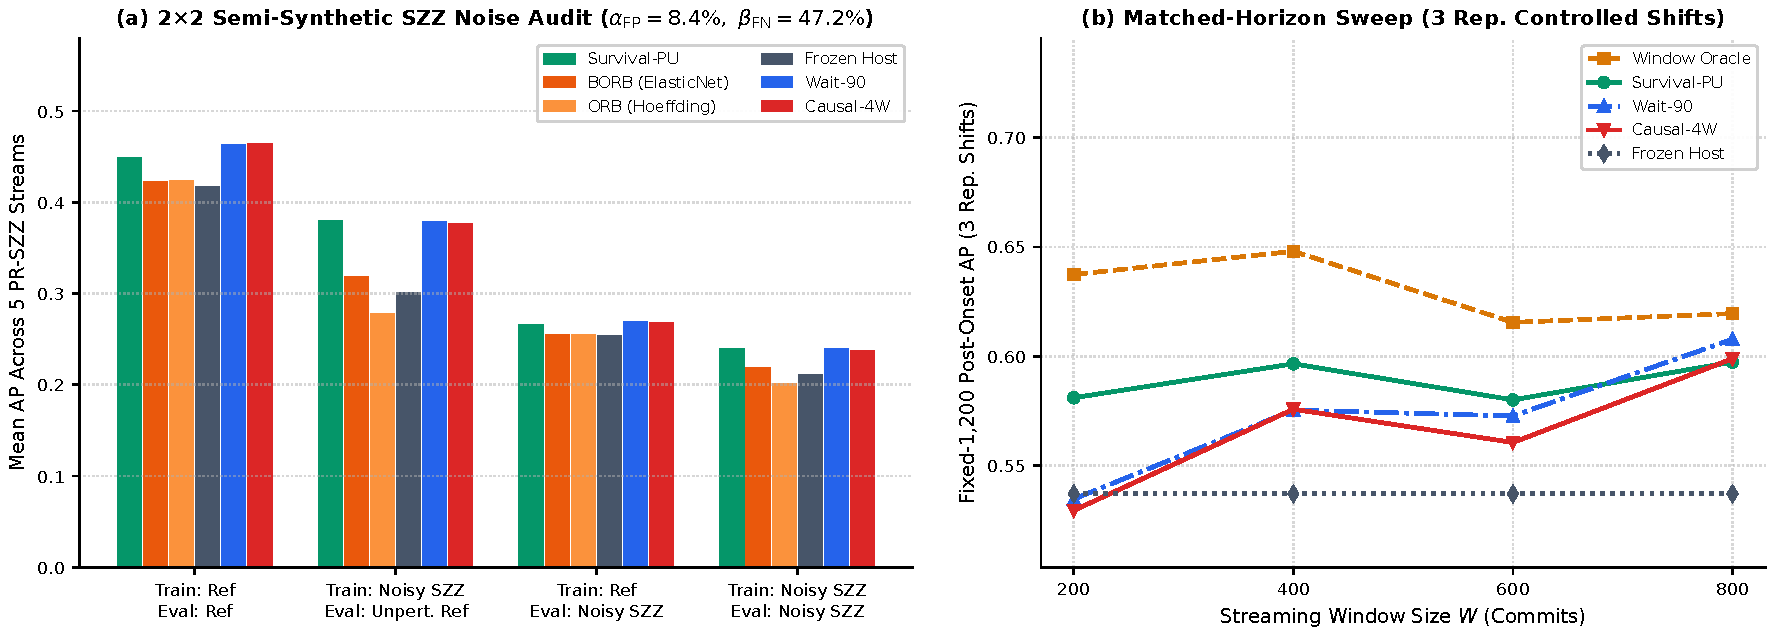
\includegraphics[width=0.98\textwidth]{fig7_szz_window_sensitivity_v3.pdf}
  \caption{(a) $2 \times 2$ frozen-prediction semi-synthetic SZZ perturbation across five PR-SZZ streams ($\alpha_{\text{FP}}=8.42\%, \beta_{\text{FN}}=47.15\%$). (b) Matched-horizon fixed 1,200-commit post-onset AP across $W \in \{200, 400, 600, 800\}$ on the three representative controlled concatenated-shift streams (Nova$\to$Zulip, Ignite$\to$Cassandra, Airflow$\to$Pulsar).}
  \label{fig:rq4_szz_win}
\end{figure}

\begin{table}[!htb]
\centering
\caption{RQ4c $2\times 2$ frozen-prediction semi-synthetic SZZ perturbation across five Bludau \& Pretschner PR-SZZ streams ($\alpha_{\mathrm{FP}}=8.42\%,\;\beta_{\mathrm{FN}}=47.15\%$, independent permanent FN noise; AP). Bold marks the highest deployable AP in each row.}
\label{tab:rq4d_szz}
\fontsize{6.6}{8.2}\selectfont
\setlength{\tabcolsep}{1.8pt}
\begin{tabular*}{\textwidth}{@{\extracolsep\fill}lcccccc@{}}
\toprule
\textbf{Train / Evaluation Cell} & \textbf{B0} & \textbf{B2-4W} & \textbf{Wait-90} & \textbf{BORB} & \textbf{ORB} & \textbf{Survival-PU} \\
\midrule
Train: PR-SZZ Ref / Eval: PR-SZZ Ref & 0.4173 & \textbf{0.4641} & 0.4639 & 0.4224 & 0.4243 & 0.4488 \\
Train: Noisy SZZ / Eval: PR-SZZ Ref & 0.3014 & 0.3768 & 0.3795 & 0.3187 & 0.2782 & \textbf{0.3802} \\
Train: PR-SZZ Ref / Eval: Noisy SZZ & 0.2542 & 0.2685 & \textbf{0.2695} & 0.2546 & 0.2556 & 0.2658 \\
Train: Noisy SZZ / Eval: Noisy SZZ & 0.2114 & 0.2377 & 0.2394 & 0.2190 & 0.2017 & \textbf{0.2397} \\
\bottomrule
\end{tabular*}
\end{table}

\textbf{RQ4c: Frozen-Prediction $2 \times 2$ Semi-Synthetic PR-SZZ Noise Perturbation.} To probe combined latency and permanent mislabeling, Table~\ref{tab:rq4d_szz} and Figure~\ref{fig:rq4_szz_win}(a) inject independent conditional flip noise over automated PR-SZZ reference labels across five streams: clean reference commits ($y_{\text{ref}} = 0$) flip to buggy at rate $\alpha_{\text{FP}} = 8.42\%$ (assigned synthetic reveal delays drawn from empirical stream latencies), and buggy reference commits ($y_{\text{ref}} = 1$) lose their fix permanently ($y_{\text{pert}} = 0, t_{\text{fix}} = +\infty$) at rate $\beta_{\text{FN}} = 47.15\%$---parameterized from project-averaged B-SZZ error rates in \citet{bludau2026quantifying} (Tables~4--5). Under this specific independent perturbation model (which does not capture feature- or age-dependent SZZ error correlation), training on noisy labels and evaluating on unperturbed PR-SZZ reference labels produces a family-level separation: window-replay and maturity-weighted batch methods cluster within $0.0034$ AP---\textbf{Survival-PU ($0.3802$)}, $\text{Wait-}90$ ($0.3795$, $+0.0007$ descriptive gap), and $B_2\text{-4W}$ ($0.3768$)---whereas online stream learners degrade substantially more (ElasticNet $\text{BORB}$: $0.4224 \to 0.3187$; Hoeffding $\text{ORB}$: $0.4243 \to 0.2782$). Generalizing this robustness beyond independent synthetic noise requires future validation on manually verified SZZ subsets.

\textbf{RQ4d: Matched-Horizon Window Sweeps and Hyperparameter Sensitivity.} Figure~\ref{fig:rq4_szz_win}(b) evaluates window size $W \in \{200, 400, 600, 800\}$ on the matched fixed-1,200 post-onset horizon across the three representative controlled shift streams in our ten-stream subset (Nova$\to$Zulip, Ignite$\to$Cassandra, and Airflow$\to$Pulsar; full 4-shift comparison including \texttt{OS Nova$\to$Neutron} in Table~\ref{tab:shift_4streams}). Here $\text{Survival-PU}$ leads deployable methods at narrow and medium windows---$W=200$ ($0.5810$ vs.\ $0.5347$ $\text{Wait-}90$ and $0.5296$ $B_2\text{-4W}$), $W=400$ ($0.5966$ vs.\ $0.5758$ $B_2\text{-4W}$; averaging these three shifts vs.\ $0.5591$ across all four shifts), and $W=600$ ($0.5801$ vs.\ $0.5727$ $\text{Wait-}90$). \textbf{At $W=800$, however, $\text{Wait-}90$ ($0.6078$) and $B_2\text{-4W}$ ($0.5989$) exceed $\text{Survival-PU}$ ($0.5974$)} once wide windows span older matured history (and across full-stream 10-stream AP for $W \in \{200..800\}$, $B_2\text{-4W}$ leads at $0.5521\text{--}0.5705$ vs.\ $0.5320\text{--}0.5543$ for $\text{Survival-PU}$). Sweeping anchor shrinkage $m_0 \in \{0, 25, 50, 100\}$ ($0.5447\text{--}0.5567$ AP) and tail cap $\gamma_{\text{tail}} \in [0.65, 0.94]$ ($\text{Brier}_{\text{cal}} \in [0.1692, 0.1716]$) confirms low sensitivity.

\begin{figure}[!htb]
  \centering
  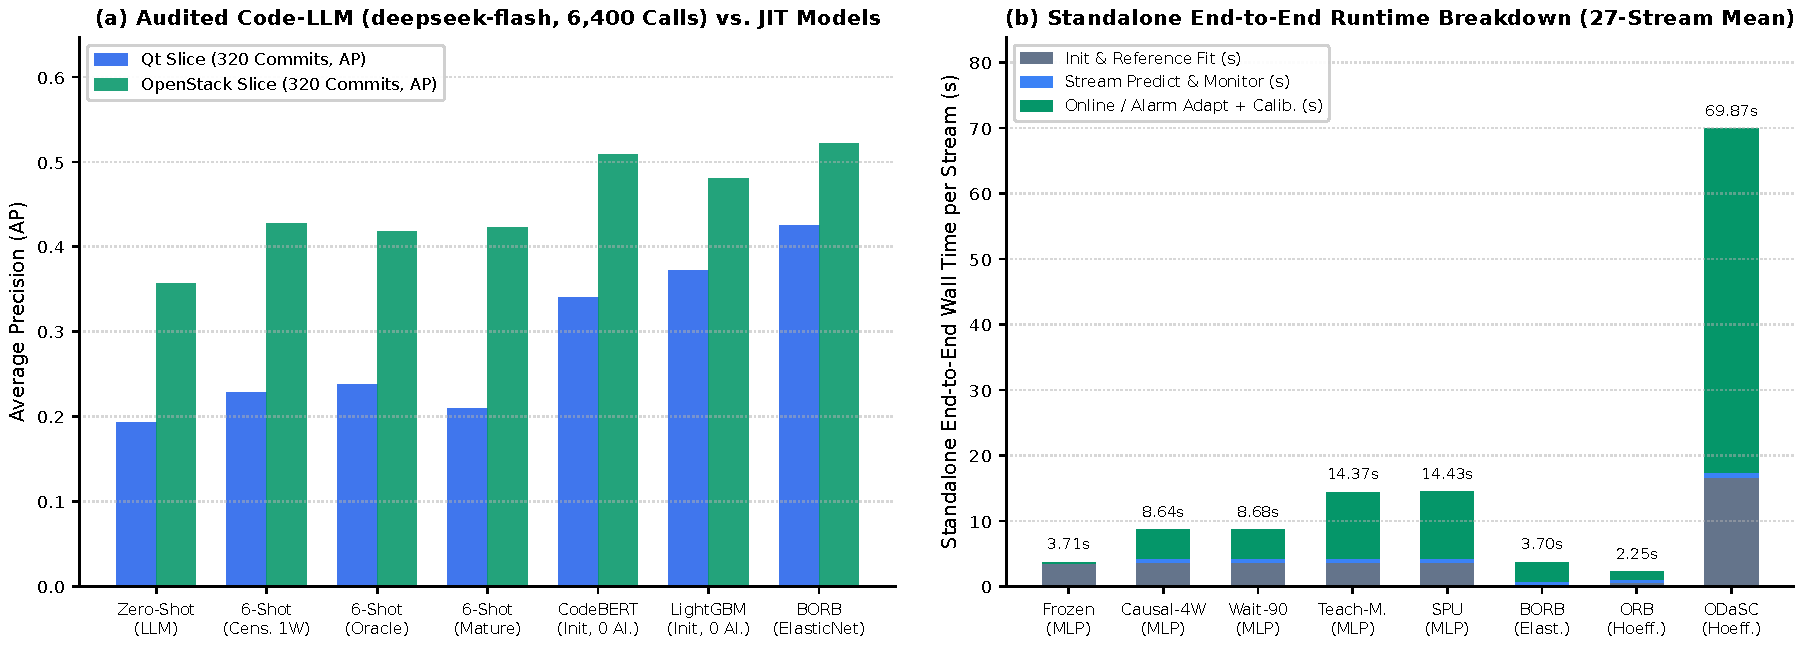
\includegraphics[width=0.98\textwidth]{fig8_llm_and_runtime_forensics_v3.pdf}
  \caption{(a) Paired prompting case study (\texttt{deepseek-flash} on 320-commit Qt and OpenStack slices) vs.\ domain-trained JIT predictors (initial checkpoints for CodeBERT/LightGBM, 0 alarms on slice). (b) Standalone wall-clock runtime on pre-extracted features across 27 natural Benchmark~B streams.}
  \label{fig:rq4f_rt}
\end{figure}

\textbf{RQ4e: Paired Code-LLM Prompting Case Study (Does In-Context Learning Bypass the Causal Wall?).} To probe whether parameter-free in-context learning (ICL) sidesteps weight-retraining censoring, we conducted a paired prompting case study using \texttt{deepseek-flash} on 320-commit slices of Qt and OpenStack ($640$ distinct commits evaluated across prompt regimes and three exemplar seeds, totaling $6{,}400$ logical evaluations; full table, model settings, and sampling protocol in Appendix~\ref{app:audits}, Table~\ref{tab:rq4f_llm}; overview in Figure~\ref{fig:rq4f_rt}(a)). Comparing strictly paired 6-shot prompts sharing identical exemplar commits and order but differing solely in observable $y_{\text{obs}}(t)$ versus eventual $y^*$ ($0.424$ flipped positives/prompt on Qt; $1.165$ on OpenStack) shows that exemplar censoring depresses thresholded $F_1$ on OpenStack from $0.4946$ to $0.3876$ ($-10.70$ points; Qt: $0.2938 \to 0.2856$), whereas \textbf{OpenStack AP is slightly higher under censored 6-shot ($0.4277 \pm 0.0152$ SD across three exemplar seeds) than paired oracle 6-shot ($0.4177 \pm 0.0299$ SD; Qt: $0.2282 \pm 0.0109$ vs.\ $0.2378 \pm 0.0166$ SD)}, mirroring Proposition~\ref{prop:bias}'s probability-shift pattern. Because this case study covers one lightweight model, 640 commits where zero DriftLens alarms fired, and historical public repositories that may overlap LLM pretraining corpora, it demonstrates only that exemplar label visibility alters prompting classification on this model rather than establishing general Code-LLM ICL claims; on both slices, domain-trained JIT predictors outperform every prompting regime in AP ($0.3401\text{--}0.5788$).

\rqbox{Summary for RQ4}{At $\kappa=3.0\times$, \texttt{FixedCurve-PU} achieves top deployable AP ($0.5547$) and raw Brier/ECE ($0.1693 / 0.0973$), whereas \texttt{Survival-PU} outperforms $B_2\text{-4W}$, both post-hoc $B_2$ controls, and \texttt{FixedCurve-PU} on threshold-tuned $F_{1,\text{th}}$ ($0.5022$ raw; $0.4898$ Platt) and fixed-$0.5$ $F_1$ ($0.5259$), while also beating \texttt{FixedCurve-PU} across all reported metrics at $\kappa=0\times$. Applying 90-day Platt calibration to the $65.9\%$-censored pool worsens calibration relative to raw scores across methods (with \texttt{Survival-PU} most resilient post-Platt). Block bootstrap cuts validation-pool null alarms $4.8\times$ and detects shifts $3\times$ faster than periodic $3W$ ($350$ vs.\ $1{,}050$ commits; $0/20$ missed). Batch window/PU methods resist independent SZZ noise better than \texttt{BORB}/\texttt{ORB}, and exemplar censoring depresses \texttt{deepseek-flash} OpenStack $F_1$ ($0.4946 \to 0.3876$).}

% ----------------------------------------------------------------------------
% 6.5 RQ5
% ----------------------------------------------------------------------------
\subsection{RQ5: Runtime Telemetry and Paired Equal-Cap Budget Error Analysis}
\label{sec:rq5}

\begin{table}[!htb]
\centering
\caption{RQ5 phase-decomposed wall-clock runtime telemetry on pre-extracted tabular features (milliseconds per stream, mean across 27 natural Benchmark B streams), separating standalone model/monitor execution from incremental shared-backbone suite cost. Bold marks the lowest standalone runtime.}
\label{tab:rq5_runtime}
\fontsize{6.4}{7.9}\selectfont
\setlength{\tabcolsep}{1.5pt}
\begin{tabular*}{\textwidth}{@{\extracolsep\fill}lrrrrrr@{}}
\toprule
\textbf{Method} & \textbf{Pred.} & \textbf{Mon.} & \textbf{Adapt} & \textbf{Calib.} & \textbf{Stand.\ E2E} & \textbf{Incr.\ E2E} \\
\midrule
B0 (Frozen MLP) & 30.6 & 0.0 & 0.0 & 201.2 & 3705.9 & 201.4 \\
B2-4W (Censored MLP) & 89.8 & 555.9 & 4159.4 & 187.1 & 8639.4 & 4405.9 \\
Wait-90 (MLP) & 88.9 & 555.9 & 4192.1 & 193.5 & 8677.7 & 4444.1 \\
Pure-nnPU (MLP) & 88.7 & 555.9 & 4369.7 & 222.5 & 8884.0 & 4650.4 \\
Teacher-Only Matched (MLP) & 90.8 & 555.9 & 9879.5 & 199.8 & 14373.2 & 10139.7 \\
Survival-PU (MLP) & 89.6 & 555.9 & 9939.3 & 196.4 & 14428.4 & 10194.9 \\
\midrule
BORB ElasticNet (Track 2) & 734.4 & 0.0 & 2712.5 & 186.5 & 3698.2 & 3698.2 \\
ORB Hoeffding (Track 2) & 567.9 & 0.0 & 954.1 & 189.9 & \textbf{2246.0} & 2246.0 \\
ODaSC Hoeffding (Track 2) & 734.3 & 0.0 & 52272.2 & 187.1 & 69871.0 & 69871.0 \\
\bottomrule
\end{tabular*}
\end{table}

\begin{table}[!htb]
\centering
\caption{RQ5 paired defect trade-off (\texttt{Survival-PU} minus \texttt{B2-4W}; seed 42) under fixed-$0.5$ thresholding, equal-cap whole-stream (\textbf{Wh.}) and per-window 400-commit (\textbf{Win.}) budgets, plus 5-seed windowed 20\%-LOC recall delta ($\Delta\mathrm{WinR}_{20}$). Realized LOC consumption is $20.0\%/20.0\%$ on 7/8 rows ($20.0\%/19.8\%$ on OS LightGBM); under Top-10\% commit budgets, $\mathrm{Net\,FP} = -\mathrm{Net\,TP}$.}
\label{tab:rq5_paired_budget}
\fontsize{5.5}{6.9}\selectfont
\setlength{\tabcolsep}{0.8pt}
\begin{tabular*}{\textwidth}{@{\extracolsep\fill}lrrrrrrr@{}}
\toprule
\textbf{Ecosystem: Host} & \textbf{Net TP$_{0.5}$} & \textbf{Net FP$_{0.5}$} & \textbf{Wh.\,10\%} & \textbf{Win.\,10\%} & \textbf{Wh.\,20\%L} & \textbf{Win.\,20\%L} & \textbf{5s $\Delta$WinR$_{20}$} \\
\midrule
Qt: Attention-CNN & +446 & +1838 & +4 & +8 & -38 & +4 & -0.0001 \\
Qt: CodeBERT & +418 & +2923 & -76 & -38 & -124 & -22 & -0.0028 \\
Qt: DeepJIT-CNN & +512 & +3211 & -54 & -1 & -123 & +15 & +0.0248 \\
Qt: LightGBM & +510 & +2430 & +120 & +124 & +31 & +31 & +0.0250 \\
\midrule
OS: Attention-CNN & +43 & +236 & -33 & +1 & -20 & +3 & -0.0073 \\
OS: CodeBERT (0 Alarms) & 0 & 0 & 0 & 0 & 0 & 0 & 0.0000 \\
OS: DeepJIT-CNN & +146 & +357 & +5 & +1 & +32 & +10 & +0.0198 \\
OS: LightGBM & +26 & +130 & -67 & +1 & -33 & -3 & +0.0025 \\
\bottomrule
\end{tabular*}
\end{table}

\textbf{Cached Execution vs.\ Feature-Encoding Runtime Telemetry.} Table~\ref{tab:rq5_runtime} and Figure~\ref{fig:rq4f_rt}(b) report phase-decomposed wall-clock runtimes on pre-extracted tabular features across 27 natural Benchmark~B streams ($5.99$ alarms/stream), charging every alarm-triggered method its standalone dependency chain ($3{,}474.1\text{ ms}$ anchor + $173.2\text{ ms}$ monitor). Standalone $\text{Survival-PU}$ executes in $14.43\text{ s}$/stream ($\approx 1.66\text{ s}$/alarm), matching step-matched $\text{Teacher-Only}$ ($14.37\text{ s}$). Online Hoeffding $\text{ORB}$ ($2.25\text{ s}$), frozen $B_0$ ($3.71\text{ s}$), and ElasticNet $\text{BORB}$ ($3.70\text{ s}$) run fastest, whereas Hoeffding $\text{ODaSC}$ requires $69.87\text{ s}$/stream due to per-event tree updates and DenStream micro-cluster radius maintenance. On multimodal Qt ($25{,}704$ commits), cached $\text{Survival-PU}$ execution takes $18.19\text{ s}$ on CPU LightGBM ($20.2$ alarms; seed-averaged alarm-step $p_{50}=0.80\text{ s}$, $p_{95}=1.07\text{ s}$, max $=1.14\text{ s}$) and $7.26\text{ s}$ on RTX~4080 GPU CodeBERT ($1.2$ alarms; $p_{50}=p_{95}=\text{max}=1.32\text{ s}$). \textbf{Adding offline GPU CodeBERT batch feature encoding ($37.32\text{ s}$ on Qt; $19.32\text{ s}$ on OpenStack) yields $44.58\text{ s}$ total batch processing on Qt}---distinct from unbatched CI webhook latency.

\textbf{Paired Whole-Stream vs.\ Per-Window Equal-Cap Budget Net Gain (Table~\ref{tab:rq5_paired_budget}).} Showing only directional rescue stories cannot establish net review yield, and allocating budgets across a multi-year retrospective stream answers a different question than matching sprint-level operational capacity. Table~\ref{tab:rq5_paired_budget} therefore reports a seed-42 commit-level diagnostic audit comparing \texttt{Survival-PU} minus $B_2\text{-4W}$ across (i) unmatched fixed-$0.50$ thresholding, (ii) equal-cap retrospective whole-stream budgets (Top-10\% commits and 20\% LOC), and (iii) equal-cap operational per-window $400$-commit budgets (Top-10\% commits and 20\% LOC per window), corroborated by 5-seed multi-seed windowed 20\%-LOC recall ($\Delta\text{WinR}_{20}$). Under 20\%-LOC budgets, commits are ranked by descending risk density $\hat{p}/\text{LOC}$ (ties: smaller LOC) and selected greedily without splitting commits while $\sum \text{LOC} \le 0.20\,\text{LOC}_{\text{total}}$, yielding equal budget caps with closely matched realized consumption ($20.0\% / 20.0\%$ on 7/8 rows and $20.0\% / 19.8\%$ on OS LightGBM; Top-10\% commit counts are exact):
\begin{itemize}[leftmargin=1.6em,itemsep=0.06em]
  \item \textit{Fixed Threshold ($0.50$, Unmatched Volume):} Preventing posterior collapse rescues $+418$ to $+512$ defects on Qt and $+26$ to $+146$ on OpenStack, at the cost of $+1{,}838$ to $+3{,}211$ extra clean commits on Qt ($+130$ to $+357$ on OpenStack).
  \item \textit{Whole-Stream Retrospective vs.\ Per-Window Operational Budgets:} Directly paralleling Section~\ref{sec:rq2}'s granularity finding, retrospective whole-stream selection penalizes \texttt{Survival-PU} heavily on Qt DeepJIT-CNN ($-54$ Top-10\%, $-123$ 20\%-LOC), Qt Att-CNN ($-38$ LOC), OS Att-CNN ($-33 / -20$), and OS LightGBM ($-67 / -33$). Switching to \textbf{operational per-window 400-commit budgets} eliminates or reverses nearly every steep whole-stream loss: Qt LightGBM remains strongly positive ($+124$ Win-10\%, $+31$ Win-20\%L; 5-seed $\Delta\text{WinR}_{20} = +0.0250$), Qt DeepJIT-CNN flips to $+15$ Win-20\%L ($-1$ Win-10\%; 5-seed $+0.0248$), OS DeepJIT-CNN stays positive ($+1 / +10$; 5-seed $+0.0198$), and Qt Att-CNN ($+8 / +4$; 5-seed $-0.0001$) and OS LightGBM ($+1 / -3$; 5-seed $+0.0025$) turn near-even, while Qt CodeBERT remains negative ($-38 / -22$; 5-seed $-0.0028$). Qualitative Tier-1 SZZ rescue illustrations ($22$ filtered Qt CodeBERT commits, $B_2\text{-4W} \in [0.0518, 0.0871]$ vs.\ $\text{SPU} \in [0.9543, 0.9754]$, plus FN/FP churn distributions) are archived in Appendix Table~\ref{tab:rq5_forensics}.
\end{itemize}

\rqbox{Summary for RQ5}{On cached features, \texttt{ORB} ($2.25\text{ s}$) and \texttt{BORB} ($3.70\text{ s}$) run fastest, \texttt{Survival-PU} takes $14.43\text{ s}$/stream ($44.58\text{ s}$ including Qt CodeBERT batch encoding), and \texttt{ODaSC} takes $69.87\text{ s}$. Under equal budget caps (exact Top-10\% commit counts; closely matched realized 20\%-LOC consumption), retrospective whole-stream selection penalizes \texttt{Survival-PU} on 5/7 alarmed hosts, whereas operational per-window 400-commit budgeting reverses most steep losses (corroborated by 5-seed $\Delta\text{WinR}_{20}$: $+0.0250$ Qt LightGBM, $+0.0248$ Qt DeepJIT-CNN, $+0.0198$ OS DeepJIT-CNN) while remaining host-dependent (negative on Qt CodeBERT).}

% ============================================================================
% 7. Discussion, Observed Operating Boundaries, and Limitations
% ============================================================================
\section{Discussion, Observed Operating Boundaries, and Limitations}
\label{sec:discussion}

We synthesize our findings around the three questions framing this study, avoiding verbatim repetition of Section~\ref{sec:results}.

\subsection{What Label-Visibility Timing Changes}
\label{sec:disc_timing}

Our audit separates two questions often conflated in drift-triggered JIT-SDP \citep{pote2026adaptive}: \textit{whether small-window retraining beats freezing} ($B_{1b}^*$ vs.\ $B_0$) and \textit{whether future-fix leakage inflates retrained weights} ($B_{1b}^*$ vs.\ $B_2\text{-4W}$). On long multi-year tabular streams ($K=25$), leaking future SZZ fixes significantly inflates whole-stream AP on both MLP and LightGBM. On two other regimes, however, even window-oracle $B_{1b}^*$ fails to surpass frozen $B_0$ or causal $B_2\text{-4W}$ on MLP: low-prevalence multimodal Benchmark~A (where frozen \texttt{Full-LR} leads, echoing \citet{zeng2021deep}) and the short confirmatory ApacheJIT cohort (where Standalone-3 prevalence is much higher at $44.6\%\text{--}48.5\%$, while horizon length, initialization scale, low $1W$ censoring, and project identity shift jointly). Finally, chronological evaluation must disclose end-of-archive follow-up limits (Appendix Tables~\ref{tab:followup_audit}--\ref{tab:followup_sensitivity}) alongside upstream repository-key artifacts such as \texttt{apachejit\_total.csv}'s $11{,}964$-commit clean \texttt{apache/hadoop} split (Table~\ref{tab:confirmatory_funnel}).

\subsection{What Complex Maturity Correction Adds Over Simpler Causal Baselines}
\label{sec:disc_increment}

Once strict causal visibility ($t \le t_{\text{alarm}}$) is enforced, our multi-track controls pinpoint where three-stage \texttt{Survival-PU} delivers genuine value and where simpler baselines suffice:
\begin{itemize}[leftmargin=1.6em,itemsep=0.06em]
  \item \textit{Whole-Stream vs.\ Within-Window Granularity:} On gradual $K=25$ streams, \texttt{Full-LR Adapt-4W}, $B_2\text{-4W}$, $\text{Wait-}90$, and \texttt{FixedCurve-PU} lead whole-stream AP over \texttt{Survival-PU}. Yet our 5-seed cross-window comparability diagnostic (Table~\ref{tab:window_ap_scale}) reverses the mean whole-stream deficit against $B_2\text{-4W}$ via within-window standardization, while leaving per-window means close across $\text{Wait-}90$, \texttt{FixedCurve-PU}, and \texttt{Full-LR}.
  \item \textit{Non-Monotonic Cross-Stage Error Propagation:} On strictly unrevealed commits ($y_{\text{obs}}=0$, Table~\ref{tab:mechanism_audit}), adaptive cohort incidence estimates Stage-1 maturity $\hat{c}(a)$ more accurately than \texttt{FixedCurve-PU} and reduces soft-target Brier over de-weighted teachers. However, \texttt{FixedCurve-PU} attains slightly lower Stage-2 prior MAE and unrevealed Brier, showing that better Stage-1 estimation does not automatically lower downstream error across coupled stages.
  \item \textit{Heavy Latency, Scale-Fair Controls, and Calibration Caution:} Under $\kappa=3\times$ latency (Table~\ref{tab:rq4a_posthoc_b2}), neither post-hoc $B_2$ control matches \texttt{Survival-PU}'s threshold-tuned $F_{1,\text{th}}$ recovery, and adaptive Stage~1 simultaneously protects against \texttt{FixedCurve-PU}'s $\kappa=0\times$ misspecification. On probabilistic accuracy, Stage~3's class weight $\omega_{+,\text{teach}} > 1$ explains why \texttt{Survival-PU}'s raw outputs trail $B_2\text{-4W}$ and \texttt{FixedCurve-PU} (whose downward censoring/target bias partially cancels $\omega_+ > 1$, matching Proposition~\ref{prop:bias}). More broadly, because raw probabilities outperform 90-day Platt calibration under $65.9\%$ pool censoring, our calibration result serves primarily as a warning against blind 90-day Platt scaling and highlights maturity-aware post-hoc calibration as a key open problem.
\end{itemize}

\subsection{Equal-Cap Inspection Cost, Observed Patterns vs.\ Exploratory Hypotheses, and Scope Limits}
\label{sec:disc_implications}

Translating ranking shifts into code-review impact depends sharply on budget granularity (Table~\ref{tab:rq5_paired_budget}): preventing fixed-$0.5$ recall collapse rescues hundreds of defects only by flagging thousands of clean commits, and retrospective whole-stream budgeting penalizes \texttt{Survival-PU} on 5/7 alarmed Benchmark~A hosts. Under realistic per-window 400-commit sprint budgets (equal budget caps with closely matched realized LOC consumption), however, steep losses vanish or turn positive on Qt LightGBM, Qt DeepJIT-CNN, and OpenStack DeepJIT-CNN (corroborated by 5-seed $\Delta\text{WinR}_{20}$), while remaining negative on Qt CodeBERT.

Because deployers cannot observe future latency multipliers ($\kappa$) or shift horizons beforehand, Table~\ref{tab:decision_matrix} separates \textbf{Part~I: Directly Observed Empirical Patterns} from \textbf{Part~II: Exploratory Hypotheses (Not Validated Selection Rules)}. For benchmark designers, three practices follow directly: enforce $t_i^{\text{fix}} \le t_{\text{alarm}}$ with archive-horizon follow-up disclosure; include linear baselines, zero-fit maturity priors, post-hoc controls, and adapted stream learners \citep{cabral2019class,cabral2023borb,song2022odasc}; and pair whole-stream AP with per-window AP, scale-normalized AP, and operational per-window equal-cap budget net TP counts.

\begin{table}[!htb]
\centering
\caption{Synthesis separating (Part~I) directly observed empirical patterns across our evaluated cohorts from (Part~II) exploratory hypotheses and prospective considerations (not validated deployment selection rules).}
\label{tab:decision_matrix}
\fontsize{6.0}{7.3}\selectfont
\renewcommand{\arraystretch}{1.04}
\setlength{\tabcolsep}{1.9pt}
\begin{tabularx}{\textwidth}{L{2.30cm}L{2.05cm}Y Y}
\toprule
\textbf{Evaluated Cohort / Factor} & \textbf{Top Observed Methods} & \textbf{Observed Empirical Evidence (Part I)} & \textbf{Scope Boundary / Exploratory Hypothesis (Part II)} \\
\midrule
\multicolumn{4}{l}{\textit{Part I: Directly Observed Empirical Patterns Within Evaluated Benchmarks}} \\
\midrule
Merged-commit archival multimodal streams (Bench~A, 13 authoring metrics) & \textbf{Full-LR Frozen}, \textbf{LApredict Frozen} & \texttt{Full-LR} ($0.3653$ AP) and \texttt{LApredict} ($0.3601$) lead all deployable neural/tree hosts (best single host: \texttt{DeepJIT-CNN} $B_0 = 0.3531$). & Within Track-1 hosts, \texttt{SPU} recovers fixed-$0.5$ $F_1$ ($0.2907$); operational per-window equal-cap budget yield is host-dependent (Table~\ref{tab:rq5_paired_budget}). \\
Gradual multi-year tabular streams ($K=25$ clusters) & \textbf{Full-LR Adapt-4W}, \textbf{B2-4W}, \textbf{FixedCurve-PU}, \textbf{BORB} & Whole-stream AP: \texttt{Full-LR} ($0.5108$, $p_{\text{Holm}}=0.0639$), $B_2\text{-4W}$ ($0.5004$), $\text{Wait-}90$ ($0.4982$), \texttt{FixedCurve-PU} ($0.4942 > 0.4866$ \texttt{SPU}, $p_{\text{Holm}}=0.0295$). \texttt{BORB} leads $F_{1,\text{th}}$ ($0.5144$). & On 5-seed predictions, within-window standardization reverses the whole-stream mean gap vs.\ $B_2\text{-4W}$ (Rank-Norm: $0.5027$ vs.\ $0.4989$; Z-Norm: $0.4990$ vs.\ $0.4968$); per-window AP also shows a small non-significant edge ($0.5246$ vs.\ $0.5192$, unadjusted $p=0.0569$; Table~\ref{tab:window_ap_scale}). \\
Controlled concatenated shifts (4 streams) & \textbf{Survival-PU} (full) / \textbf{BORB-Alarm} (first 1.2k) & Full post-onset AP: \texttt{SPU} ($0.5764$) $>$ \texttt{ODaSC-Host} ($0.5727$). First 1,200c: \texttt{BORB-Alarm} ($0.5931$) $>$ \texttt{SPU} ($0.5591$). & Concatenated 1-hour splices ($23.7\%\text{--}60.0\%$ cross-boundary fixes) differ from natural drift; at $W=800$ on 3 shifts, $\text{Wait-}90$ ($0.6078$) overtakes \texttt{SPU} ($0.5974$). \\
Latency extremes ($\kappa=0\times, 3\times$) & \textbf{Survival-PU} ($F_1$/$F_{1,\text{th}}$), \textbf{FixedCurve-PU} ($3\times$ AP/raw Br.), $B_2\text{-4W}$ ($0\times$ AP) & $\kappa=0\times$: $B_2\text{-4W}$ ($0.5974$) $>$ \texttt{SPU} ($0.5760$) $>$ Fix ($0.5544$). $\kappa=3\times$: \texttt{SPU} leads tuned $F_{1,\text{th}}$ ($0.5022$) and $F_1$ ($0.5259$); Fix leads AP ($0.5547$) and raw Brier/ECE ($0.1693 / 0.0973$). & Raw scores beat 90d Platt under $65.9\%$ pool censoring (\texttt{SPU} is most resilient post-Platt); feature-dependent post-hoc calibration remains untested, and density-ratio omission remains an unvalidated simplification candidate not evaluated under extreme $\kappa$. \\
Independent semi-synthetic SZZ noise (5 PR-SZZ streams) & \textbf{Survival-PU}, \textbf{Wait-90}, \textbf{B2-4W} & Independent $\alpha_{\text{FP}}=8.42\%, \beta_{\text{FN}}=47.15\%$: batch methods cluster ($0.3768\text{--}0.3802$) well above \texttt{BORB} ($0.3187$) and \texttt{ORB} ($0.2782$). & Scoped to independent synthetic flips over automated PR-SZZ labels; feature- or age-dependent real SZZ noise remains untested. \\
\midrule
\multicolumn{4}{l}{\textit{Part II: Exploratory Hypotheses \& Prospective Considerations (Not Validated Selection Rules)}} \\
\midrule
Confirmatory repos ($N < 3{,}000$; Standalone-3 primary vs.\ Umbrella-4) & \textbf{ODaSC} (OHT), \textbf{BORB} (ENet), \textbf{ORB} (OHT) & Standalone-3 (unsplit): \texttt{ODaSC} $=0.7857$, $B_{1b}^* = 0.5951 < B_2\text{-4W} = 0.5985 < B_0 = 0.6565$. Frozen Umbrella-4: \texttt{ODaSC} $=0.8289$, $B_{1b}^* = 0.6801 < B_2\text{-4W} = 0.6858$ (LightGBM $0.7020$ vs.\ $0.6976$ n.s.). & \textit{Unvalidated hypothesis:} \texttt{HDFS*}/\texttt{MapReduce*} omit $11{,}964$ clean commits into \texttt{apache/hadoop}; horizon, prevalence, censoring, and project identity remain confounded on Standalone-3. \\
\bottomrule
\end{tabularx}
\end{table}

\textbf{Scope Limitations.} Six limitations bound our conclusions: (1) Benchmark~A orders merged Git revisions by \texttt{author\_date} rather than live Gerrit patch-set-1 uploads, and archive observation horizons $T_{\text{end}}$ are observable proxies rather than certified collection cutoffs; (2) Stage~1 assumes local trailing-cohort stationarity (I1--I2), Stage~2 uses heuristic shrinkage, and Eq.~\eqref{eq:ht_prev}'s outer $\pi_{\max}=0.70$ clamp causes unreachable bisection when alarm-time $\bar{y}_{\text{obs},\mathcal{B}_{\text{cal}}} > 0.70$ ($28.6\%\text{--}30.0\%$ of alarms on \texttt{HDFS*}); (3) 90-day causal Platt calibration retains $27\%\text{--}66\%$ censoring under multi-month lag and worsens post-Platt calibration at $\kappa=3\times$ (Section~\ref{sec:rq4}); (4) RQ4b's null alarm rate resamples the calibration validation pool rather than independent stationary production streams; (5) controlled concatenated shifts impose a 1-hour splice with $23.7\%\text{--}60.0\%$ cross-boundary fixes; and (6) RQ4e is a single-model (\texttt{deepseek-flash}), 640-commit prompting case study on public commits predating LLM pretraining cutoffs.

% ============================================================================
% 8. Threats to Validity
% ============================================================================
\section{Threats to Validity}
\label{sec:threats}

\textbf{Construct Validity.} SZZ back-tracing is susceptible to tangled commits, refactorings, and unlinked fixes \citep{dacosta2017framework,rosa2021evaluating,fan2021impact}, while archival collections also experience end-of-archive censoring ($t_i^{\text{fix}} > T_{\text{end}}$). We mitigated construct threats by quarantining Tier-3 and retroactive links ($t_{\text{fix}} < t_{\text{commit}}$) to $+\infty$, auditing remaining follow-up across all 34 natural repository streams plus full Benchmark~A $\ge 180\text{d}/\ge 365\text{d}$ sensitivity (Appendix Tables~\ref{tab:followup_audit}--\ref{tab:followup_sensitivity}), disclosing upstream \texttt{apachejit\_total.csv}'s $11{,}964$-commit clean \texttt{apache/hadoop} split (Table~\ref{tab:confirmatory_funnel}), verifying paired whole-stream and per-window equal-cap budget net TP counts (Table~\ref{tab:rq5_paired_budget}), and reporting \texttt{LOC-Only} overlap alongside whole-stream, per-window, and scale-normalized AP.

\textbf{Internal Validity.} All 41 method execution branches passed deterministic pipeline prefix-invariance testing ($0.0$ historical perturbation error), though prefix invariance certifies leak-free code execution rather than upstream commit-time feature provenance. We separated protocol-specified development analyses ($K=25$) from the pre-unlock frozen confirmatory cohort, disclosed the post-unlock $N < 4{,}000$ sizing amendment and its exact splits, treated $B_{1b}^*$ strictly as a Pote-inspired counterfactual rather than a verbatim original-repo reproduction, and verified all $1{,}452$ empirical table cells across $22$ tables, locked parameters, exact-path prose comparisons, and quantifier/relational claim guards automatically (Appendix~\ref{app:repro}).

\textbf{External and Conclusion Validity.} Our adapted Track-2 implementations (ElasticNet-\texttt{BORB}, OHT-\texttt{ORB}, OHT-\texttt{ODaSC}) reflect specific base learners rather than entire algorithmic paradigms, and independent synthetic SZZ flips do not capture feature-dependent real SZZ errors. Formal $\alpha=0.05$ Holm--Bonferroni inference is scoped strictly to $K=25$ and $K=24$ natural donor clusters (distinct from the exploratory unadjusted $p$-values in Table~\ref{tab:window_ap_scale}; Section~\ref{sec:metrics_protocol}), and failed MLP directional replication on Phase~C (both unsplit Standalone-3 and frozen Umbrella-4) is reported directly without post hoc retuning.

% ============================================================================
% 9. Conclusion
% ============================================================================
\section{Conclusion}
\label{sec:conclusion}

Unsupervised drift monitors remove label dependence when deciding \textit{when} to flag shifts, not when \textit{supervising} model updates under multi-month SZZ verification latency. Across multi-year ecosystems, 68.8\%--94.6\% of defects inside scheduled 400-commit windows remain unrevealed at update time. Consequently, leaking future fixes inflates whole-stream AP significantly across $K=25$ donor clusters on both MLP ($+0.0237$, $p_{\text{Holm}} = 6.63 \times 10^{-5}$) and LightGBM ($+0.0476$, $p_{\text{Holm}} = 3.70 \times 10^{-5}$), while circular block-bootstrap calibration cuts validation-pool null alarms $4.8\times$ and detects abrupt shifts $3\times$ faster than periodic schedules.

Our cross-paradigm audit demonstrates that no single adaptive strategy dominates all regimes. Frozen linear models lead deployable Benchmark~A; simpler causal baselines ($B_2\text{-4W}$, $\text{Wait-}90$, \texttt{FixedCurve-PU}) significantly outperform cohort-fitted \texttt{Survival-PU} on gradual $K=25$ whole-stream AP (reversing the mean $B_2\text{-4W}$ gap non-significantly under within-window score standardization); ElasticNet \texttt{BORB} leads $K=25$ $F_{1,\text{th}}$ and early post-shift recovery; and Hoeffding \texttt{ODaSC} leads the short confirmatory cohort (Standalone-3: $0.7857$; Umbrella-4: $0.8289$), where MLP hindsight optimism fails to replicate. Within these clear operating boundaries, \texttt{Survival-PU} offers targeted advantages on full post-shift AP ($0.5764$), LightGBM soft-target distillation, and classification resilience across both latency extremes---preventing \texttt{FixedCurve-PU}'s $\kappa = 0\times$ misspecification and beating $B_2\text{-4W}$, two post-hoc $B_2$ controls, and \texttt{FixedCurve-PU} on threshold-tuned $F_{1,\text{th}}$ ($0.5022$) at $\kappa = 3\times$. Finally, our calibration audit warns that standard 90-day Platt scaling degrades probabilities when calibration pools suffer heavy censoring; developing maturity-aware post-hoc calibration and prospectively validating deployment-observable selection rules remain central priorities for adaptive JIT-SDP.

\backmatter

% ============================================================================
% Declarations (Springer Nature / Software Quality Journal Standard)
% ============================================================================
\section*{Declarations}
\begin{itemize}[leftmargin=1.5em,itemsep=0.12em]
  \item \textbf{Funding:} This research received no external funding.
  \item \textbf{Conflict of interest:} The authors declare that they have no conflict of interest.
  \item \textbf{Competing interests:} The authors declare no competing financial or non-financial interests that are relevant to the content of this article.
  \item \textbf{Ethics approval and consent to participate:} Not applicable; this study analyzes publicly available open-source software repository histories without human-subject experimentation.
  \item \textbf{Consent for publication:} Not applicable.
  \item \textbf{Availability of data, code, and artifacts:} The complete replication package---including immutable \texttt{src\_v3/} modules, \texttt{scripts\_v3/} post-processing, companion audit, and verification runners, pinned \texttt{requirements\_\allowbreak lock\_\allowbreak v3.txt}, \texttt{LICENSE} (MIT), SHA-256 manifests for all 94 stream bundles and CodeBERT caches, 50 commit-level \texttt{.npz} prediction archives, lossless archived LLM exchange logs, and automated verifiers---is publicly available at \url{https://github.com/789748456v/CausalJIT-Audit-SQJ} and accompanied by a full offline archival bundle for permanent Zenodo deposit upon acceptance.
  \item \textbf{Author contributions:} Z.L.: Conceptualization, Methodology, Software, Data Curation, Formal Analysis, Writing -- Original Draft. S.X.: Software, Validation, Data Curation, Writing -- Review \& Editing. K.L.: Validation, Investigation, Visualization, Writing -- Review \& Editing. S.M.: Formal Analysis, Investigation, Writing -- Review \& Editing. F.G.: Validation, Visualization, Writing -- Review \& Editing. Y.Z.: Supervision, Conceptualization, Methodology, Project Administration, Writing -- Review \& Editing. All authors read and approved the final manuscript.
\end{itemize}

% ============================================================================
% Appendices
% ============================================================================
\begin{appendices}
\renewcommand{\theHtable}{\thesection.\arabic{table}}

\section{Executed Host Architectures, Soft-Target GBDT Proof, and Traceability}
\label{app:repro}

Table~\ref{tab:backbone_specs} documents the exact executed constructors and training budgets in \texttt{src\_v3/\allowbreak models\_\allowbreak and\_\allowbreak baselines\_\allowbreak v3.py}. All neural models optimize with \texttt{AdamW} (weight decay $10^{-4}$, batch size $128$, gradient-norm clip $1.0$, deterministic CuDNN). Token vocabularies ($8{,}000$ tokens), TF-IDF/SVD projections ($48$-D msg + $64$-D diff = $112$-D SVD), and $z$-score scalers fit \textbf{strictly on $[0, n_{\text{init}})$}, whereas initial host weights and optional tabular linear-residual skips (\texttt{init\_\allowbreak linear\_\allowbreak skip\_\allowbreak from\_\allowbreak data}) train on the causal pre-stream prefix $[0, n_{\text{init}}+n_{\text{val}})$ using observable labels $y_{\text{obs}}(t_{\text{start}})$. For LightGBM, DriftLens computes $24$-D PCA Gaussian Fr\'echet distances on the concatenation of the leading $\min(D, 48)$ standardized features and the initial booster's exact raw margin $x_{i,1:\min(D,48)} \oplus [f_{\text{raw}}(x_i) + z_{\text{init}}]$.

\begin{proposition}[Analytical Margin Derivatives for Soft-Target GBDT]
\label{prop:lgbm}
For $\mathcal{L}_{\text{SPU},i}(z_i) = u_i[\omega_+ q_i \log(1 + e^{-z_i}) + (1 - q_i)\log(1 + e^{z_i})]$ with $q_i \in [0, 1]$, $u_i > 0$, and margin $z_i = z_{\text{init}} + \sum_{m=1}^M T_m(x_i)$, the exact first and second derivatives with respect to $z_i$ are $g_i = u_i[(1 + (\omega_+ - 1)q_i)\sigma(z_i) - \omega_+ q_i]$ and $h_i = u_i(1 + (\omega_+ - 1)q_i)\sigma(z_i)(1 - \sigma(z_i)) > 0$. Passing $z_{\text{init}}$ as the training initial margin and adding $z_{\text{init}}$ to raw tree margins at inference preserves exact split-gain margins for continuous $q_i \in [0, 1]$ without dataset duplication.
\end{proposition}

\begin{proof}
Differentiating $\mathcal{L}_{\text{SPU},i}(z_i)$ via $\frac{d}{dz}\log(1+e^{-z}) = \sigma(z)-1$ and $\frac{d}{dz}\log(1+e^z) = \sigma(z)$ yields $g_i$ and $h_i = \partial g_i/\partial z_i$. Because LightGBM excludes training initial scores from raw tree sums at prediction time, adding $z_{\text{init}}$ restores $z_i$ (verified in our pre-unlock gate to match native hard-label LightGBM within $1.19 \times 10^{-7}$ max float32 host margin error).
\end{proof}

\begin{table}[!htb]
\centering
\caption{Executed architectural, DriftLens monitoring-space, and optimization specifications across all five host predictors (\texttt{src\_v3/models\_and\_baselines\_v3.py}).}
\label{tab:backbone_specs}
\fontsize{5.8}{7.0}\selectfont
\renewcommand{\arraystretch}{1.02}
\setlength{\tabcolsep}{1.6pt}
\begin{tabularx}{\textwidth}{L{1.55cm}L{1.85cm}Y L{1.95cm}L{2.55cm}}
\toprule
\textbf{Host Model} & \textbf{Causal Input Features} & \textbf{Architecture \& Linear-Residual Skip} & \textbf{DriftLens Space ($24$-D PCA)} & \textbf{Executed Init \& Per-Alarm Budgets} \\
\midrule
Attention-CNN \citep{pote2026adaptive} & $64$ msg + $128$ diff tokens + $13$ authoring metrics & $64$-D dual emb.; $k\in\{1,2,3\}$ 1D-CNN ($48$ filters $\to 144$-D); $6$-head self/cross-attn; $192\to 64$-D ($\text{drop}=0.30$) + frozen Tab-13 LR skip & $64$-D penultimate LayerNorm-\allowbreak ReLU vector $z_i$ & AdamW ($\text{bs}=128$); Init: $12$ ep., $\text{lr}=7{\times}10^{-4}$; Alarm ($\text{lr}=4.5{\times}10^{-4}$): $5$ ep.\ ($B_{1/2}$/Wait/ODaSC-H), $6$ ep.\ ($\text{nnPU}$), $4{+}4$ ep.\ ($\text{SPU}$/Fixed), or step-matched \texttt{max\_\allowbreak opt\_\allowbreak steps} \\
CodeBERT \citep{feng2020codebert} & $768$-D msg + $768$-D diff (\texttt{codebert-\allowbreak base}) + $13$ metrics & Dual $128$-D LayerNorm-\allowbreak GELU adapters + $4$-head bimodal self-attn + $|a_m-a_c| \oplus (a_m\odot a_c) \to 160 \to 64$-D ($\text{drop}=0.25$) + frozen Tab-13 LR skip & $64$-D penultimate LayerNorm-\allowbreak GELU vector $z_i$ & AdamW ($\text{bs}=128$); Init: $12$ ep., $\text{lr}=8{\times}10^{-4}$; Alarm ($\text{lr}=4.5{\times}10^{-4}$): $5$ ep.\ ($B_{1/2}$/Wait/ODaSC-H), $6$ ep.\ ($\text{nnPU}$), $4{+}4$ ep.\ ($\text{SPU}$/Fixed), or step-matched \texttt{max\_\allowbreak opt\_\allowbreak steps} \\
DeepJIT-CNN \citep{hoang2019deepjit} & $64$ msg + $128$ diff tokens + $13$ metrics & $64$-D dual emb.; parallel $k\in\{1,2,3\}$ 1D-CNNs ($64$ filters) + $48$-D metric MLP $\to 64$-D ($\text{drop}=0.25$) + frozen Tab-13 LR skip & $64$-D penultimate LayerNorm-\allowbreak GELU vector $z_i$ & AdamW ($\text{bs}=128$); Init: $12$ ep., $\text{lr}=7{\times}10^{-4}$; Alarm ($\text{lr}=4.5{\times}10^{-4}$): $5$ ep.\ ($B_{1/2}$/Wait/ODaSC-H), $6$ ep.\ ($\text{nnPU}$), $4{+}4$ ep.\ ($\text{SPU}$/Fixed), or step-matched \texttt{max\_\allowbreak opt\_\allowbreak steps} \\
Tabular MLP (Benchmark B/C) & Standardized commit-time / PR-SZZ metrics ($D$-dim) & LayerNorm-\allowbreak GELU ($D\to 128$) + residual block ($128\to 128$) $\to 64$-D head ($\text{drop}=0.20$) & $64$-D penultimate LayerNorm-\allowbreak GELU vector $z_i$ & AdamW ($\text{bs}=128$); Init: $12$ ep., $\text{lr}=8{\times}10^{-4}$; Alarm ($\text{lr}=4.5{\times}10^{-4}$): $5$ ep.\ ($B_{1/2}$/Wait/ODaSC-H), $6$ ep.\ ($\text{nnPU}$), $4{+}4$ ep.\ ($\text{SPU}$/Fixed), or step-matched \texttt{max\_\allowbreak opt\_\allowbreak steps} \\
LightGBM \citep{ke2017lightgbm} & $112$-D msg+diff SVD + $13$ metrics (or $D$ tab.) & Callable-objective GBDT (Prop.~\ref{prop:lgbm}), $\text{num\_leaves}=15$, $\text{lr}=0.05$, subsample $0.85$, colsample $0.85$, $\ell_1=0.1, \ell_2=1.0$ & $[x_{i,1:\min(D,48)}, z_i]$ with exact \texttt{init\_score} margin $z_i$ & Init: $90$ rounds; Alarm: fresh $75$-tree fit ($B_{1/2}$/Wait/ODaSC-H/Teach-Exact), fresh $75{+}75$ fits ($\text{SPU}$/Fixed), fresh $150$-tree fit (\texttt{Teach-\allowbreak Matched}); 2 threads \\
\bottomrule
\end{tabularx}
\end{table}

\textbf{Executed Competitor Specifications (\texttt{src\_v3/\allowbreak stream\_\allowbreak competitors\_\allowbreak v3.py}).}
\begingroup\raggedright
\begin{itemize}[leftmargin=1.6em,itemsep=0.08em]
  \item \texttt{ORB\_\allowbreak OHT\_\allowbreak Native} \citep{cabral2019class}: Ensemble of $10$ \texttt{river.\allowbreak tree.\allowbreak Hoeffding\allowbreak TreeClassifier} learners ($\text{grace\_period}=200$, $\delta = 10^{-7}$, $\tau = 0.05$, \texttt{leaf\_\allowbreak prediction="nba"}) trained via OzaBagging \citep{oza2005online} on strict $t_{\text{event}} < t_{\text{commit}}$ verification-latency events ($\text{waiting\_days} = 90.0$ clean maturity events plus revealed fix events), with exact feature-tuple duplicate clean-count noise filtering ($\text{count} > 5$ skipped prior to $p_1$ updates, matching \texttt{jitsdp/\allowbreak baseline.py}), EMA decay $0.99$, prediction-rate window $100$, $th=0.40, l_0=10, l_1=12, m=1.5$, and cold-start $0.0$ output until both classes are observed.
  \item \texttt{BORB\_\allowbreak Native} \& \texttt{BORB\_\allowbreak Alarm} \citep{cabral2023borb}: Single \texttt{SGDClassifier} (\texttt{loss=\allowbreak "log\_loss"}, \texttt{penalty=\allowbreak "elasticnet"}, $\alpha=0.02$, \texttt{l1\_ratio}$=0.15$, \texttt{learning\_\allowbreak rate=\allowbreak "optimal"}) refreshed every $200$ commits (\texttt{BORB\_\allowbreak Native}) or strictly post-window upon DriftLens alarms (\texttt{BORB\_\allowbreak Alarm}), running $20$ inner skewed-resampling \texttt{partial\_fit} iterations ($\text{max\_sample\_size} = 2{,}000$, $th=0.40, l_0=10, l_1=12, m=1.5$) over all historical revealed positives ($t_{\text{fix}} \le t$) and unfixed commits aged $\ge 90.0$ days.
  \item \texttt{ODaSC\_\allowbreak OHT\_\allowbreak Native} \citep{song2022odasc}: Ensemble of $10$ \texttt{river} Hoeffding trees ($\text{grace\_period}=200, \delta=10^{-7}, \tau=0.05$) consuming two-stage $t_{\text{event}} < t_{\text{commit}}$ events with $\text{waiting\_days} = 15.0$ provisional-negative horizon and \texttt{SongDenStream\allowbreak ConfidenceTracker} one-sided micro-cluster label confidences ($\delta_{\text{thresh}} = 0.85$, radius $\epsilon_r$ initialized from the $15$th pairwise distance percentile on $[0, \min(s_0, 250))$) across all $D$ features.
  \item \texttt{Pure\_nnPU} \citep{kiryo2017positive}: Disjoint historical confirmed-positive set $P$ and $4W$ unlabeled marginal pool $U$ trained with non-negative PU risk ($\beta = 0.0, \gamma = 1.0$; $6$ neural epochs or unit pseudo-Hessian GBDT steps) using clipped inverse-maturity shrunk prior $\hat{\pi}_{\text{target}}$ on $4W$.
\end{itemize}
\endgroup

\textbf{Code-to-Manuscript Traceability Mapping (\texttt{src\_v3/} and \texttt{scripts\_v3/}).} The following mapping links protocol concepts in Sections~\ref{sec:method}--\ref{sec:threats} to their implementation symbols and archived artifacts:
\begingroup\raggedright
\begin{itemize}[leftmargin=1.6em,itemsep=0.06em]
  \item \textit{Stage 1--3 Estimators \& Training:} Risk-eligible cohort incidence is implemented by \texttt{Cohort\allowbreak Incidence\allowbreak Estimator} and its $145$-knot fallback \texttt{\_set\_fallback()} in \texttt{src\_v3/\allowbreak survival\_\allowbreak estimators\_\allowbreak v3.py}; clipped inverse-maturity shrunk prevalence by \texttt{estimate\_\allowbreak ht\_\allowbreak shrunk\_\allowbreak prevalence}; shared Bayesian posterior by \texttt{compute\_\allowbreak survival\_\allowbreak pu\_\allowbreak posterior}; neural/GBDT host fitting by \texttt{train\_\allowbreak supervised\_\allowbreak v3} and \texttt{LightGBM\allowbreak HostV3} in \texttt{src\_v3/\allowbreak models\_\allowbreak and\_\allowbreak baselines\_\allowbreak v3.py}; and three-branch causal calibration by \texttt{calibrate\_\allowbreak causal\_\allowbreak stream\_\allowbreak probs\_\allowbreak strict} in \texttt{src\_v3/\allowbreak stream\_\allowbreak competitors\_\allowbreak v3.py}.
  \item \textit{Data Bundles, Split Rules, \& Codified Constants:} Stream sizing is implemented by \texttt{compute\_\allowbreak split\_\allowbreak sizes} and confirmatory unlocking via \texttt{data\_\allowbreak audit\_\allowbreak v3.py -{-}unlock-\allowbreak confirmatory}; codified interpretation rules and forensic rules reside in \texttt{PRE\_\allowbreak REGISTERED\_\allowbreak INTERPRETATION\_\allowbreak BOUNDARIES} and \texttt{V3\_CONFIG.\allowbreak forensic\_rules} (\texttt{Tier1\_\allowbreak McIntosh\_\allowbreak CSV}) in \texttt{src\_v3/\allowbreak config\_\allowbreak v3.py}; natural multimodal bundles are \texttt{qt\_\allowbreak natural\_\allowbreak 25k} and \texttt{openstack\_\allowbreak natural\_\allowbreak 13k} (with \texttt{premerge28} sensitivity); the ten-stream subset is \texttt{REPRESENTATIVE\_\allowbreak 10\_\allowbreak STREAMS} in \texttt{src\_v3/\allowbreak run\_\allowbreak v3\_\allowbreak experiments.py} (containing shift streams \texttt{abrupt\_\allowbreak nova\_\allowbreak zulip}, \texttt{abrupt\_\allowbreak ignite\_\allowbreak cassandra}, \texttt{abrupt\_\allowbreak airflow\_\allowbreak pulsar}; Benchmark~B's fourth shift is \texttt{abrupt\_\allowbreak deepjit\_\allowbreak nova\_\allowbreak neutron\_\allowbreak pure13}). Historical RQ4 artifact filenames \texttt{rq4d\_\allowbreak szz\_\allowbreak perturbation\_\allowbreak v3.json}, \texttt{rq4e\_\allowbreak sensitivity\_\allowbreak sweeps\_\allowbreak v3.json}, and \texttt{rq4f\_\allowbreak llm\_\allowbreak audit\_\allowbreak v3.json} correspond to manuscript subsections RQ4c, RQ4d, and RQ4e.
  \item \textit{Automated Verification Suites \& Companion Controls:} Pre-unlock gate archive (\texttt{766e3fd6...}) and live post-campaign Checks 2--14 run via \texttt{scripts\_v3/\allowbreak run\_\allowbreak post\_\allowbreak campaign\_\allowbreak mechanism\_\allowbreak checks\_\allowbreak v3.py}; the matched RQ4a \texttt{FixedCurve-PU} control (\texttt{rq4a\_\allowbreak fixedcurve\_\allowbreak control\_\allowbreak v3.json}) runs via \texttt{scripts\_v3/\allowbreak run\_\allowbreak rq4a\_\allowbreak fixedcurve\_\allowbreak control\_\allowbreak v3.py}; all companion data-funnel, follow-up sensitivity, unrevealed-commit Stage 1--3, symmetrical Raw/Platt \& PostHoc Logit/Ratio (with clipping/tie-rate diagnostics), 5-seed window-AP/scale-removal, and operational equal-cap budget audits (\texttt{reviewer\_\allowbreak mechanism\_\allowbreak audits\_\allowbreak v3.json}, exact $0.00$ parity with \texttt{rq4a\_\allowbreak latency\_\allowbreak intervention\_\allowbreak v3.json}) run via \texttt{scripts\_v3/\allowbreak run\_\allowbreak reviewer\_\allowbreak mechanism\_\allowbreak audits\_\allowbreak v3.py}; all $1{,}452$ empirical table cells across $22$ tables and provenance hashes across all $15$ JSON outputs verify via \texttt{src\_v3/\allowbreak verify\_\allowbreak manuscript\_\allowbreak v3.py}; and all $33$ \texttt{V3\_CONFIG} table fields, exact-path prose claims, and quantifier/relational claim guards verify via \texttt{scripts\_v3/\allowbreak verify\_\allowbreak prose\_\allowbreak claims\_\allowbreak v3.py}.
\end{itemize}
\endgroup

\section{Additional Data-Funnel, Follow-Up, Mechanism, Shift, Prompting, and Forensics Audits}
\label{app:audits}
\setcounter{table}{0}

This appendix consolidates seven supplementary audit tables referenced in Sections~\ref{sec:benchmarks}--\ref{sec:rq5}. Tables~\ref{tab:confirmatory_funnel}--\ref{tab:followup_sensitivity} document the confirmatory ApacheJIT filtering funnel (reconciling upstream \texttt{apachejit\_total.csv}'s $11{,}964$-commit clean \texttt{apache/hadoop} split), observable archive-horizon follow-up windows across all 34 natural repository streams, and complete Benchmark~A follow-up sensitivity across $\ge 180\text{d}$ and $\ge 365\text{d}$ cutoffs.

\begin{table}[!htb]
\centering
\caption{Confirmatory ApacheJIT data-construction funnel from upstream \texttt{apachejit\_total.csv} ($106{,}674$ rows) through our chronological cutoff ($\text{author\_date} \le \text{2019-01-01}$, denoted \textbf{Cut}) to evaluation splits. Upstream assigns $11{,}964$ clean Hadoop monorepo commits to \texttt{apache/hadoop} (details in Section~\ref{sec:benchmarks}); Standalone-3 have no monorepo split.}
\label{tab:confirmatory_funnel}
\fontsize{6.0}{7.4}\selectfont
\setlength{\tabcolsep}{1.2pt}
\begin{tabular*}{\textwidth}{@{\extracolsep\fill}lrrrrrrr@{}}
\toprule
\textbf{Upstream Project Key} & \textbf{Raw $N$} & \textbf{Raw Pos} & \textbf{Raw Prev.} & \textbf{Cut $N$} & \textbf{Cut Prev.} & \textbf{Eval $N$} & \textbf{Eval Prev.} \\
\midrule
\texttt{apache/hadoop} (Monorepo Clean Only) & 11964 & 0 & 0.0\% & 10330 & 0.0\% & -- & -- \\
\midrule
\texttt{apache/hadoop-hdfs} (HDFS*) & 2907 & 2222 & 76.4\% & 2850 & 76.7\% & 1925 & 89.2\% \\
\texttt{apache/hadoop-mapreduce} (MapRed.*) & 1321 & 838 & 63.4\% & 1318 & 63.5\% & 893 & 78.8\% \\
\midrule
\texttt{apache/spark} (Standalone) & 1465 & 632 & 43.1\% & 1273 & 46.5\% & 848 & 45.6\% \\
\texttt{apache/zeppelin} (Standalone) & 1451 & 622 & 42.9\% & 1350 & 44.6\% & 900 & 55.2\% \\
\texttt{apache/zookeeper} (Standalone) & 839 & 342 & 40.8\% & 686 & 48.5\% & 461 & 49.5\% \\
\bottomrule
\end{tabular*}
\end{table}

\begin{table}[!htb]
\centering
\caption{Observable archive-horizon follow-up proxy audit across all 34 natural repository streams ($2+14+8+5+5=34$): minimum and median remaining window between evaluation commit timestamp and observable archive-horizon proxy $T_{\mathrm{end}} = \max(\max_i t_i, \max_{i:\, t_i^{\mathrm{fix}}<\infty} t_i^{\mathrm{fix}})$, plus maximum stream fraction of evaluation commits with $<90$, $<180$, or $<365$ days of follow-up.}
\label{tab:followup_audit}
\fontsize{6.0}{7.4}\selectfont
\setlength{\tabcolsep}{1.2pt}
\begin{tabular*}{\textwidth}{@{\extracolsep\fill}lrrrrrr@{}}
\toprule
\textbf{Stream Cohort} & \textbf{Streams} & \textbf{Min Rem (d)} & \textbf{Med Rem (d)} & \textbf{Max $<$90d} & \textbf{Max $<$180d} & \textbf{Max $<$365d} \\
\midrule
Bench A Natural (Qt, OS) & 2 & 0.0 & 429.4 & 7.0\% & 15.5\% & 41.0\% \\
Bench B: Cabral ICSE'19 (14) & 14 & 366.0 & 1054.0 & 0.0\% & 0.0\% & 0.0\% \\
Bench B: ApacheJIT Dev (8) & 8 & 301.9 & 1822.7 & 0.0\% & 0.0\% & 0.7\% \\
Bench B: PR-SZZ SQJ'26 (5) & 5 & 156.9 & 823.5 & 0.0\% & 2.4\% & 22.7\% \\
Phase C: Confirmatory (5) & 5 & 388.8 & 2234.9 & 0.0\% & 0.0\% & 0.0\% \\
\bottomrule
\end{tabular*}
\end{table}

\begin{table}[!htb]
\centering
\caption{Benchmark~A archive follow-up sensitivity (seed 42; 4-host mean AP and $F_1$ plus \texttt{Full-LR Frozen}) restricting evaluation to commits with $\ge 180$ or $\ge 365$ days before $T_{\mathrm{end}}$. Bold marks the best deployable value per row; pairwise shifts are detailed in Section~\ref{sec:rq2}.}
\label{tab:followup_sensitivity}
\fontsize{5.8}{7.1}\selectfont
\setlength{\tabcolsep}{1.0pt}
\begin{tabular*}{\textwidth}{@{\extracolsep\fill}lrrcccccc@{}}
\toprule
\textbf{Metric --- Slice} & \textbf{$N$} & \textbf{Prev.} & \textbf{Full-LR} & \textbf{B0} & \textbf{B1b*} & \textbf{B2-4W} & \textbf{Wait-90} & \textbf{SPU} \\
\midrule
AP --- Qt (All) & 18204 & 5.4\% & \textbf{0.2248} & 0.2008 & 0.2048 & 0.1859 & 0.1631 & 0.1833 \\
AP --- Qt ($\ge 180$d) & 15388 & 6.0\% & \textbf{0.2499} & 0.2219 & 0.2249 & 0.2069 & 0.1831 & 0.2038 \\
AP --- Qt ($\ge 365$d) & 10747 & 6.1\% & \textbf{0.2545} & 0.2283 & 0.2260 & 0.2143 & 0.1900 & 0.2045 \\
AP --- OS (All) & 3704 & 14.7\% & \textbf{0.4097} & 0.3756 & 0.3231 & 0.3333 & 0.3025 & 0.2964 \\
AP --- OS ($\ge 180$d) & 3698 & 14.7\% & \textbf{0.4113} & 0.3773 & 0.3247 & 0.3352 & 0.3042 & 0.2983 \\
AP --- OS ($\ge 365$d) & 2578 & 16.1\% & \textbf{0.4488} & 0.4101 & 0.4005 & 0.3850 & 0.3841 & 0.3903 \\
\midrule
$F_1$ --- Qt (All) & 18204 & 5.4\% & 0.2311 & 0.0515 & 0.2521 & 0.0284 & 0.1947 & \textbf{0.2406} \\
$F_1$ --- Qt ($\ge 180$d) & 15388 & 6.0\% & 0.2567 & 0.0526 & 0.2743 & 0.0301 & 0.2027 & \textbf{0.2642} \\
$F_1$ --- Qt ($\ge 365$d) & 10747 & 6.1\% & 0.2628 & 0.0635 & 0.2767 & 0.0364 & 0.2005 & \textbf{0.2635} \\
$F_1$ --- OS (All) & 3704 & 14.7\% & \textbf{0.4408} & 0.0687 & 0.1961 & 0.1465 & 0.1965 & 0.2051 \\
$F_1$ --- OS ($\ge 180$d) & 3698 & 14.7\% & \textbf{0.4422} & 0.0688 & 0.1967 & 0.1467 & 0.1970 & 0.2061 \\
$F_1$ --- OS ($\ge 365$d) & 2578 & 16.1\% & \textbf{0.4863} & 0.0673 & 0.1664 & 0.1264 & 0.1544 & 0.1634 \\
\bottomrule
\end{tabular*}
\end{table}

Table~\ref{tab:mechanism_audit} audits Stage~1--3 intermediate accuracy across all 62 fired DriftLens alarms on the 10-stream subset ($74{,}400$ pool evaluations across $59{,}600$ unique commits), separating strictly unrevealed commits ($y_{\text{obs}}=0$) from the all-pool positive-writeback control and comparing \texttt{Survival-PU} against \texttt{FixedCurve-PU}. Reference maturity $c^*(a) = |\mathcal{P}|^{-1}\sum_{j \in \mathcal{P}} \mathbb{I}(\Delta_j \le a)$ is computed over all archive-labeled positives $\mathcal{P} = \{j : y_j^* = 1\}$ in each stream (counting unlinked $t_j^{\text{fix}} = +\infty$ as unrevealed), evaluated on $\mathcal{B}_{\text{cal}}$ ages and averaged per alarm before aggregating across alarms ($n=62$) or streams ($n=10$), with all $\pm$ dispersion values reporting sample SD.

\begin{table}[!htb]
\centering
\caption{Stage 1--3 intermediate audit across 62 fired DriftLens alarms on 10 representative streams (seed 42; $74{,}400$ pool evaluations across $59{,}600$ unique commits; $c^*(a)$ and SD summaries in Section~\ref{sec:rq3} and Appendix~\ref{app:audits}). Upper rows restrict to unrevealed commits ($y_{\mathrm{obs}}=0$); the bottom row adds fair positive writeback ($y_{\mathrm{obs}}=1 \to 1.0$) to the de-weighted teacher.}
\label{tab:mechanism_audit}
\fontsize{5.6}{7.0}\selectfont
\setlength{\tabcolsep}{0.8pt}
\begin{tabular*}{\textwidth}{@{\extracolsep\fill}lrrrrrrr@{}}
\toprule
\textbf{Pool Stratum ($\mathcal{B}_{\mathrm{cal}}$)} & \textbf{Evals} & \textbf{True $\pi^*$} & \textbf{Raw Br.} & \textbf{DeWt/WB Br.} & \textbf{Fix $q_i$ Br.} & \textbf{SPU $q_i$ Br.} & \textbf{SPU Bias} \\
\midrule
Unrev.\ Young ($<30$d) & 12778 & 0.195 & 0.1861 & 0.1456 & 0.1310 & 0.1373 & +0.0282 \\
Unrev.\ Mid ($30$--$90$d) & 21741 & 0.156 & 0.1829 & 0.1319 & 0.1143 & 0.1233 & +0.0179 \\
Unrev.\ Aged ($\ge 90$d) & 30226 & 0.154 & 0.1805 & 0.1227 & 0.1194 & 0.1181 & -0.0189 \\
All Unrevealed ($y_{\mathrm{obs}}=0$) & 64745 & 0.163 & 0.1824 & 0.1303 & 0.1200 & 0.1236 & +0.0027 \\
\midrule
All Pool (+Writeback Ctrl) & 74400 & 0.271 & 0.1753 & 0.1134 & 0.1044 & 0.1076 & +0.0024 \\
\bottomrule
\end{tabular*}
\end{table}

Table~\ref{tab:shift_4streams} disaggregates all four Benchmark~B controlled concatenated shifts alongside cross-boundary fix-reveal fractions, Table~\ref{tab:rq4f_llm} presents the complete paired Code-LLM prompting case study (RQ4e), and Table~\ref{tab:rq5_forensics} archives the qualitative Tier-1 SZZ commit illustrations referenced in Section~\ref{sec:rq5}.

\begin{table}[!htb]
\centering
\caption{Per-stream breakdown across all four Benchmark~B controlled concatenated distribution-shift streams (MLP, 10 seeds): full post-onset AP (\textbf{Post}) and first 1,200 post-onset commit AP (\textbf{1.2k}). At the 1-hour splice boundary, $33.2\%$ (Nova$\to$Zulip), $60.0\%$ (Ignite$\to$Cassandra), $23.7\%$ (Airflow$\to$Pulsar), and $35.0\%$ (OS Nova$\to$Neutron) of revealed pre-onset fixes occur after the onset timestamp.}
\label{tab:shift_4streams}
\fontsize{5.6}{7.0}\selectfont
\setlength{\tabcolsep}{0.9pt}
\begin{tabular*}{\textwidth}{@{\extracolsep\fill}lcccccccc@{}}
\toprule
\textbf{Method} & \textbf{N$\to$Z Post} & \textbf{N$\to$Z 1.2k} & \textbf{I$\to$C Post} & \textbf{I$\to$C 1.2k} & \textbf{A$\to$P Post} & \textbf{A$\to$P 1.2k} & \textbf{OS Post} & \textbf{OS 1.2k} \\
\midrule
B0 (Frozen) & 0.5062 & 0.5618 & 0.7044 & 0.6618 & 0.3797 & 0.3994 & 0.4353 & 0.4287 \\
B1b* (4W Oracle) & 0.5265 & 0.5699 & 0.7955 & 0.6964 & 0.6995 & 0.6827 & 0.4332 & 0.4289 \\
\midrule
B2-4W (Censored) & 0.4758 & 0.5238 & 0.7584 & 0.6550 & 0.6074 & 0.5747 & 0.3895 & 0.3932 \\
Wait-90 & 0.4020 & 0.3981 & 0.7702 & 0.6662 & 0.6419 & 0.6362 & 0.4074 & 0.4211 \\
FixedCurve-PU & 0.4727 & 0.4727 & 0.7537 & 0.6726 & 0.6348 & 0.6341 & 0.3994 & 0.4113 \\
Survival-PU & 0.4798 & 0.4836 & 0.7641 & 0.6799 & 0.6402 & 0.6369 & 0.4214 & 0.4358 \\
ODaSC-Host & 0.4978 & 0.5607 & 0.7576 & 0.6504 & 0.6281 & 0.6119 & 0.4072 & 0.4113 \\
BORB-Alarm & 0.4808 & 0.5741 & 0.7259 & 0.7588 & 0.5339 & 0.6210 & 0.4439 & 0.4184 \\
\bottomrule
\end{tabular*}
\end{table}

\begin{table}[!htb]
\centering
\caption{RQ4e audited Code-LLM evaluation (\texttt{deepseek-flash}, $6{,}400$ logical evaluations across $6{,}819$ HTTP attempts on 320-commit Qt and OpenStack slices) vs.\ domain-trained JIT predictors (initial frozen checkpoints for alarm-triggered hosts, as $0$ alarms fired before window 2). Bold marks the best causal value per column.}
\label{tab:rq4f_llm}
\fontsize{6.4}{7.9}\selectfont
\setlength{\tabcolsep}{1.5pt}
\begin{tabular*}{\textwidth}{@{\extracolsep\fill}lcccccc@{}}
\toprule
\textbf{Model / Prompt Regime} & \textbf{Qt AP} & \textbf{Qt $F_1$} & \textbf{Qt AUC} & \textbf{OS AP} & \textbf{OS $F_1$} & \textbf{OS AUC} \\
\midrule
DeepSeek Zero-Shot (Causal) & 0.1925 & 0.1613 & 0.6565 & 0.3570 & 0.2558 & 0.7051 \\
DeepSeek 6-Shot (Censored 1W) & 0.2282 & 0.2856 & 0.6882 & 0.4277 & 0.3876 & 0.7381 \\
DeepSeek 6-Shot (Paired Oracle 1W) & 0.2378 & 0.2938 & 0.6933 & 0.4177 & 0.4946 & 0.7320 \\
DeepSeek 6-Shot (Causal Mature $\ge 90$d) & 0.2091 & 0.2984 & 0.6641 & 0.4229 & 0.5072 & 0.7470 \\
\midrule
CodeBERT + LinSkip (Init Prefix, 0 Alarms) & 0.3401 & 0.0930 & 0.7875 & 0.5083 & 0.0588 & 0.8131 \\
LightGBM SVD+Tab13 (Init Prefix, 0 Alarms) & 0.3719 & 0.1277 & \textbf{0.8110} & 0.4806 & 0.0000 & 0.8025 \\
Full-LR Adapt-4W (Tabular-13) & 0.3719 & \textbf{0.3885} & 0.7779 & \textbf{0.5788} & \textbf{0.5954} & \textbf{0.8391} \\
BORB ElasticNet (Tabular-13) & \textbf{0.4251} & 0.3687 & 0.7917 & 0.5216 & 0.5174 & 0.8133 \\
\bottomrule
\end{tabular*}
\end{table}

\textbf{RQ4e Paired Prompting Protocol Details.} The 6,400 logical evaluations in Table~\ref{tab:rq4f_llm} queried \texttt{deepseek-flash} (\texttt{temperature=0.0}, JSON schema output, $6{,}819$ HTTP attempts including $419$ retried transient transport errors and $2$ final $0.50$ fallbacks; $99.97\%$ valid-response rate, $100\%$ JSON compliance on $6{,}398$ responses, $99.95\%$ non-empty diff coverage) across the first 320 evaluation commits of natural Qt and OpenStack. Zero-shot prompts passed commit message, truncated code diff, and commit-time metrics; paired 6-shot arms sampled identical historical 1W exemplars across three random seeds differing solely in $y_{\text{obs}}(t)$ versus $y^*$, while the descriptive causal-mature arm sampled aged ($\ge 90\text{d}$) exemplars ($F_1 = 0.5072$ OS / $0.2984$ Qt).

\begin{table}[!htb]
\centering
\caption{RQ5 pre-declared SZZ-linked commit illustrations on natural Qt (CodeBERT + frozen linear skip; selected under pre-declared forensic rules requiring McIntosh--Kamei Tier-1 SZZ links; Alarm \#1 at commit $9{,}900$ had $88.19\%$ $4W$ censoring). Bold marks the highest deployable predicted risk per commit.}
\label{tab:rq5_forensics}
\fontsize{6.4}{7.9}\selectfont
\setlength{\tabcolsep}{1.5pt}
\begin{tabular*}{\textwidth}{@{\extracolsep\fill}lccccccc@{}}
\toprule
\textbf{Repo:Inducing $\to$ Fix} & \textbf{Lag (d)} & \textbf{B0} & \textbf{B1b*} & \textbf{B2-4W} & \textbf{Wait-90} & \textbf{BORB} & \textbf{Survival-PU} \\
\midrule
\texttt{qtquick1:9995a291} $\to$ \texttt{4a1505d5} & 148.2 & 0.5485 & 0.7775 & 0.0518 & 0.6608 & 0.8803 & \textbf{0.9589} \\
\texttt{qtbase:fb3f47b6} $\to$ \texttt{ac2b15bd} & 25.9 & \textbf{0.9682} & 0.9399 & 0.0519 & 0.8868 & 0.8892 & 0.9543 \\
\texttt{qtwebkit:0376f732} $\to$ \texttt{840e2817} & 181.9 & 0.5408 & 0.9744 & 0.0871 & \textbf{0.9775} & 0.6282 & 0.9754 \\
\bottomrule
\end{tabular*}
\end{table}

\textbf{RQ5 Qualitative Commit Illustrations and Churn Skew.} Applying our pre-declared Tier-1 forensic filter (lag $\ge 14\text{d}$, $B_0 \ge 0.45$, $B_2\text{-4W} \le 0.35$, $\text{SPU} \ge 0.50$) on natural Qt (CodeBERT, seed 42; Alarm~\#1 at commit $9{,}900$ had $88.19\%$ $4W$ censoring) yields $22$ rescue illustrations (Table~\ref{tab:rq5_forensics}; $0$ alarms on OpenStack CodeBERT seed 42). Across full evaluation sets, Tier-1 false-negative candidates skew smaller (Qt: $436$ FNs, median $32$ vs.\ $69$ LOC across all $981$ defects; OpenStack: $477$ FNs, median $74$ vs.\ $89$ LOC) while high-score false positives skew larger (Qt: $1{,}620$ FPs, median $65$ vs.\ $9$ LOC clean; OpenStack: $18$ FPs, median $146$ vs.\ $19$ LOC), ranging from $2$-LOC FNs (\texttt{qtmultimedia:4bb75559}) to $570{,}767$-LOC imports (\texttt{qtwebkit:d441d6f3}).

\end{appendices}

\bibliography{references}

\end{document}
